\documentclass[aspectratio=169]{beamer}
   \usetheme{metropolis}
   \setbeamertemplate{blocks}[rounded][shadow=false]
\usepackage{url}
\usepackage{hyperref}
\usepackage{booktabs}
\usepackage{tabularx}
\usepackage{dcolumn}
   \newcolumntype{d}[1]{D{.}{.}{#1}}
\usepackage{graphicx}
\usepackage[justification=raggedright]{caption}
\usepackage{adjustbox}
\usepackage{color}
\usepackage{textpos}
\usepackage{etoolbox}
\usepackage[cache=true,cachedir=minted_cache]{minted}
\usepackage{multimedia}

\captionsetup[figure]{justification=centering}

\makeatletter
\patchcmd{\beamer@sectionintoc}{\vskip1.5em}{\vskip0.5em}{}{}
\makeatother

\definecolor{smured}{rgb}{0.797,0,0.027}
\definecolor{smublue}{RGB}{48,64,116}
\definecolor{dkgreen}{rgb}{0,0.6,0}
\definecolor{gray}{rgb}{0.5,0.5,0.5}
\definecolor{mauve}{rgb}{0.58,0,0.82}
\definecolor{text_gray}{RGB}{46,58,62}

\setbeamercolor{progress bar}{fg=smured,bg=smublue}
\setbeamercolor{title separator}{fg=smublue}
\setbeamercolor{frametitle}{bg=smublue}

\metroset{
  numbering=fraction
}

\hypersetup{
  colorlinks=true,
  allcolors=text_gray,
  urlcolor=smured,
}

\addtobeamertemplate{frametitle}{}{
\begin{textblock*}{1cm}(\textwidth,-0.96cm)

\includegraphics[width=0.9cm]{figures/smu_logo.pdf}
\end{textblock*}}

\setminted{breaklines,linenos,fontsize=\scriptsize}
\setmintedinline{fontsize=auto}

\title{Overview of SMU HPC Clusters}
\author{Dr.\ Robert Kalescky\\ Dr.\ John LaGrone}
\institute{
Research and Data Sciences Services\\
Office of Information Technology\\
Center for Research Computing\\
Southern Methodist University}
\date{\today}

\begin{document}

\begin{frame}
\titlepage
\end{frame}

\begin{frame}{Outline}
\footnotesize
\tableofcontents[hideallsubsections]
\end{frame}

\section{History}

\begin{frame}{UNIVAC Computing Center}
\begin{center}
\includegraphics[width=0.875\linewidth]{figures/univac.png}
\end{center}
\end{frame}


\section{Research Support}

\begin{frame}{Research and Data Science Services}
\begin{table}
\small
\begin{tabularx}{\textwidth}{Xll}
\toprule
Domain & Name & Email \\
\midrule
Data Science & Dr.\ Eric Godat & \href{mailto:egodat@smu.edu}{egodat@smu.edu} \\
High-Performance Computing & Dr.\ Robert Kalescky & \href{mailto:rkalescky@smu.edu}{rkalescky@smu.edu} \\
& Dr.\ John LaGrone & \href{mailto:jlagrone@smu.edu}{jlagrone@smu.edu} \\
Machine Learning \& Artificial Intelligence & Dr.\ Tue Vu & \href{mailto:tuev@smu.edu}{tuev@smu.edu} \\
Custom Devices (IOT, wearables, etc.) & Guillermo Vasquez & \href{mailto:guillermov@smu.edu}{guillermov@smu.edu} \\
Human Trafficking Data Analyst & Mateo Langston-Smith & \href{mailto:mlangstonsmith@smu.edu}{mlangstonsmith@smu.edu} \\
\bottomrule
\end{tabularx}
\caption{The OIT Research and Data Science Services team provides research computing support, consultations, and collaborations.}
\end{table}
\end{frame}

\begin{frame}{Data Science Institute (DSI)}
\begin{itemize}
  \item Maintains our primary shared resource for research computing in collaboration with OIT
  \item Provides research computing tools, support, and training to all faculty, staff, and students using research computing resources
  \item \url{https://southernmethodistuniversity.github.io/hpc_docs/} has documentation and news
  \item \href{mailto:help@smu.edu}{help@smu.edu} or \href{mailto:rkalescky@smu.edu}{rkalescky@smu.edu} or \href{mailto:jlagrone@smu.edu}{jlagrone@smu.edu} for help
  \item Request an account at \url{https://southernmethodistuniversity.github.io/hpc_docs/}
\end{itemize}
\end{frame}


\section{Supercomputing}

%\begin{frame}{Moore's Law}
%\begin{itemize}
%\item Historically, we have depended on hardware advances to enable faster and
%      larger simulations
%\item In 1965, Gordon Moore observed that the CPU and RAM transistor count
%      about doubled each year
%\item ``Moore’s Law'' has since been revised to a doubling once every 2 years,
%      with startling accuracy
%\item Physical limits, e.g. power consumption, heat emission, and even the size
%      of the atom, have currently stopped this expansion on individual processors,
%      with speeds that have leveled off since around 2008
%\end{itemize}
%\end{frame}

\begin{frame}{Growth in CPU Transistor Counts}
\begin{figure}
  \centering
  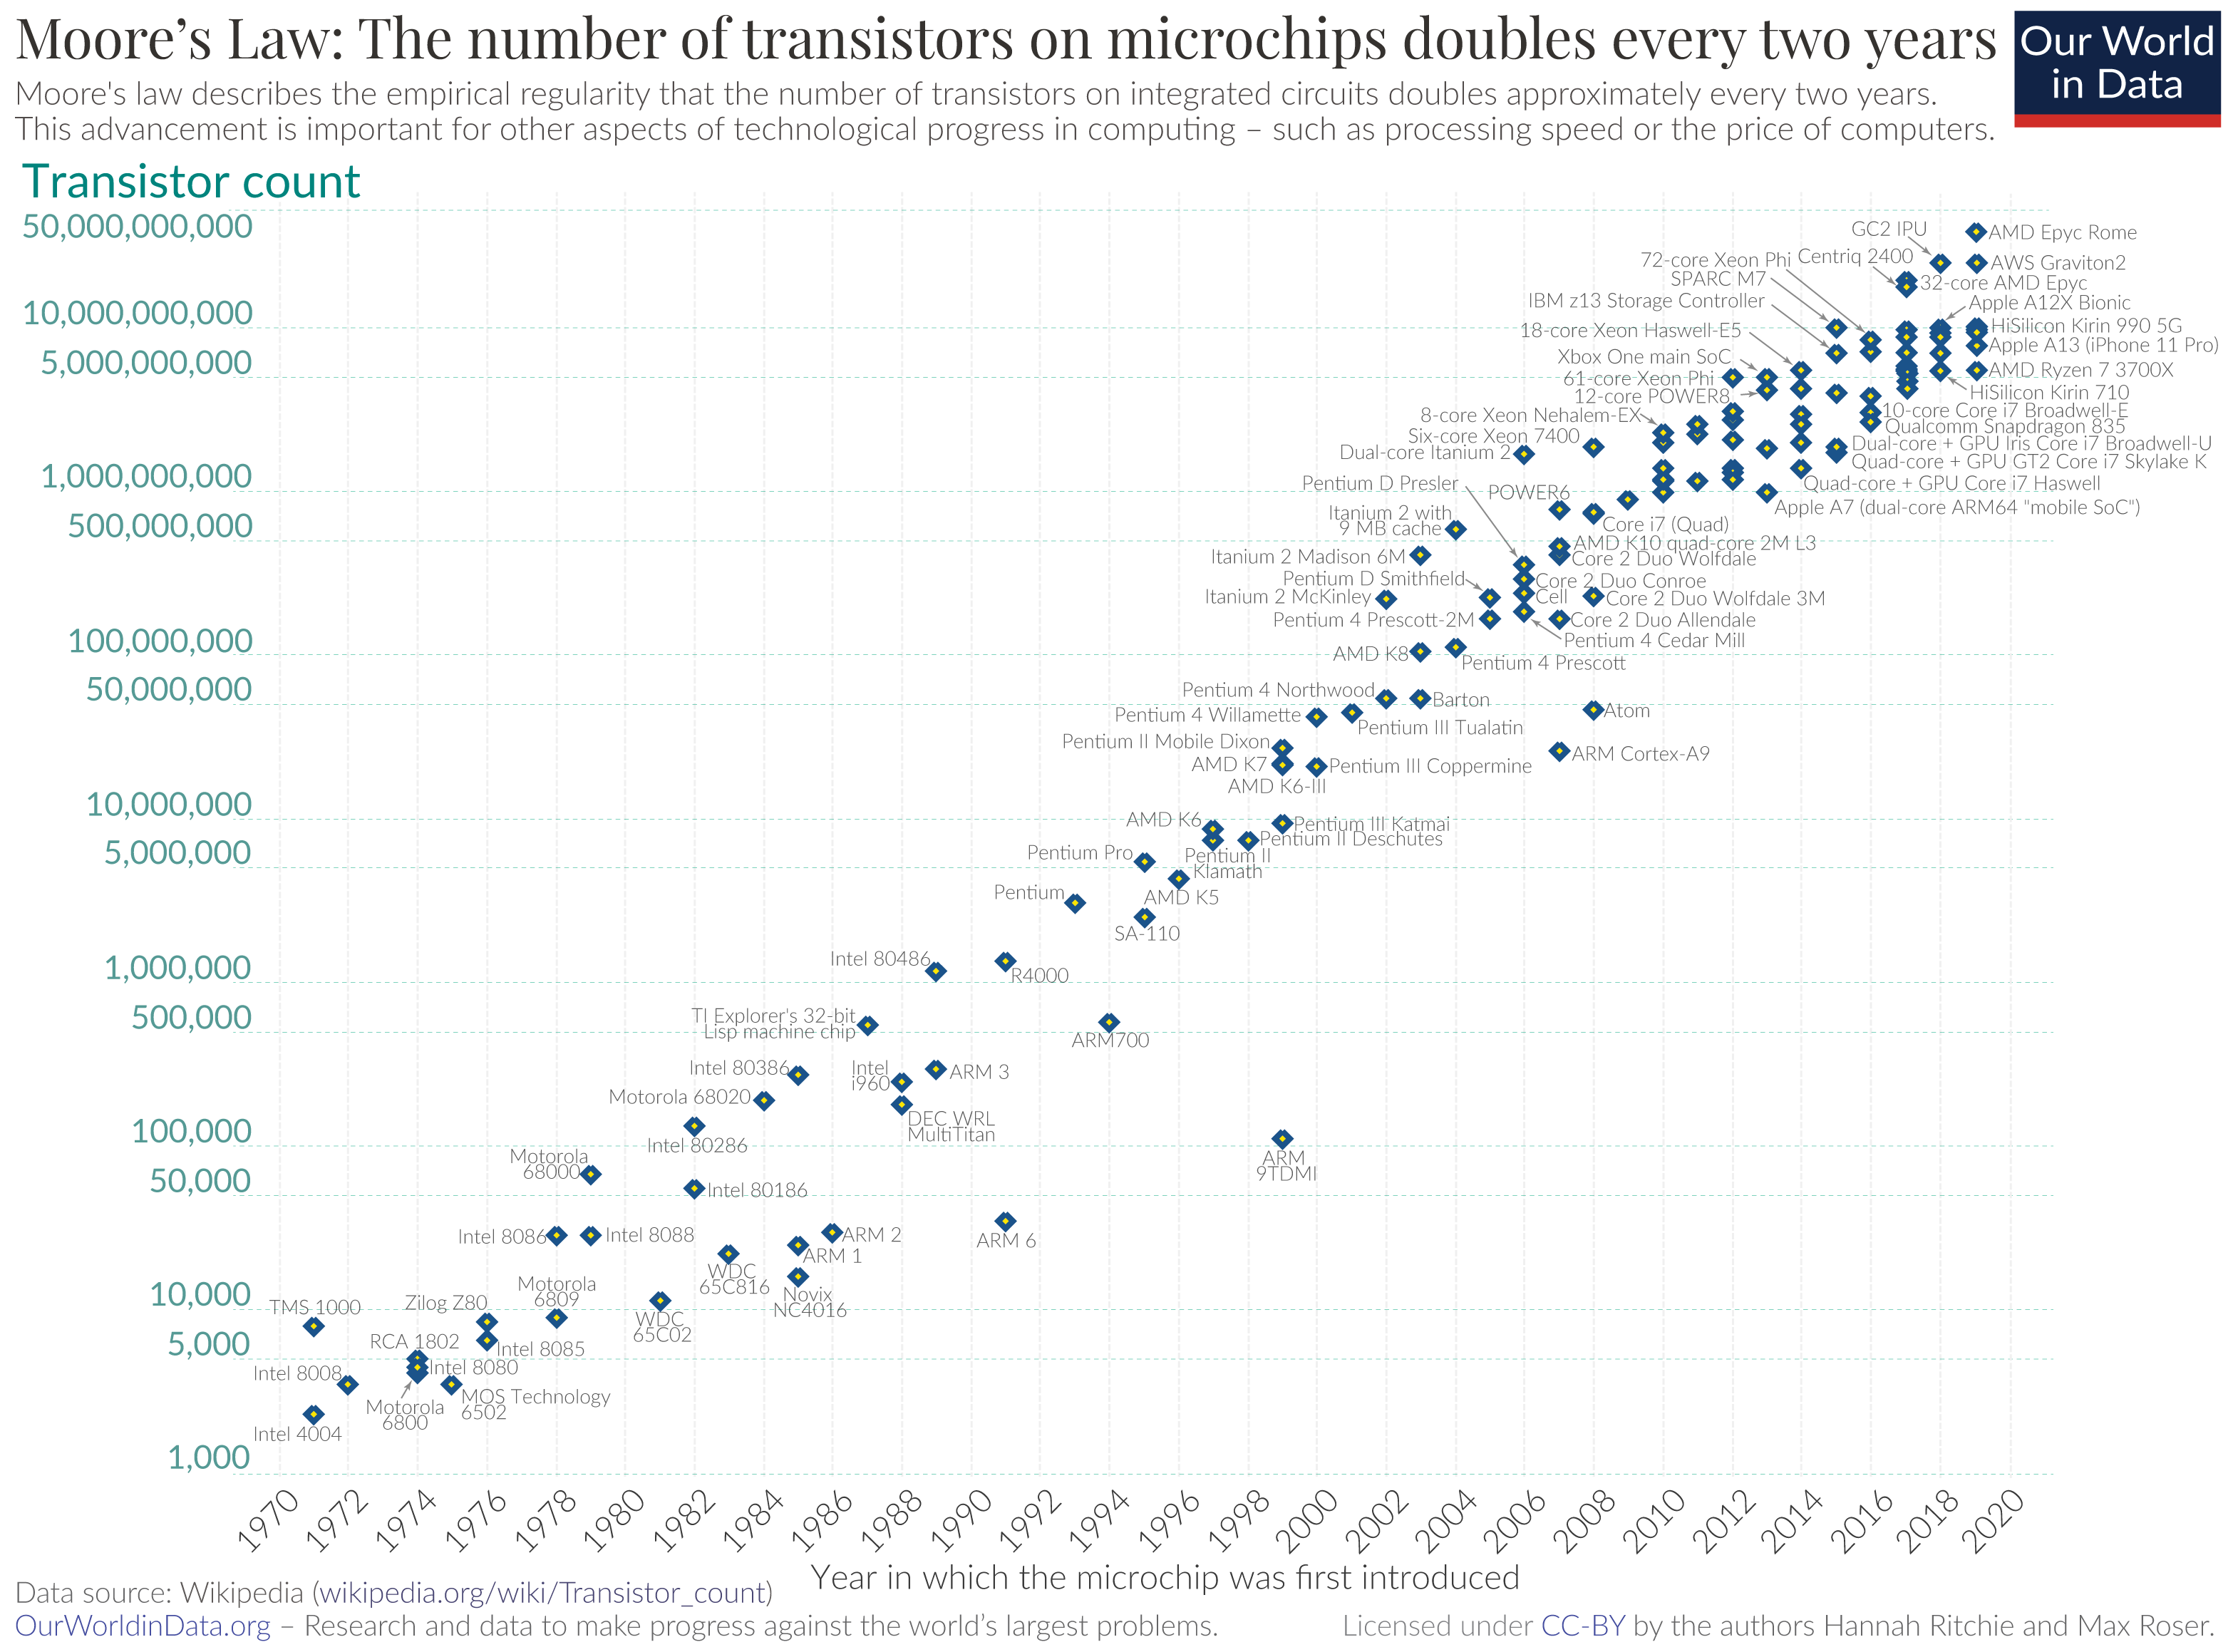
\includegraphics[width=0.65\linewidth]{figures/cpu_transistor_counts.png}
\end{figure}
\end{frame}

%\begin{frame}{Decrease in Cost Per FLOPS}
%\begin{figure}
%  \centering
%  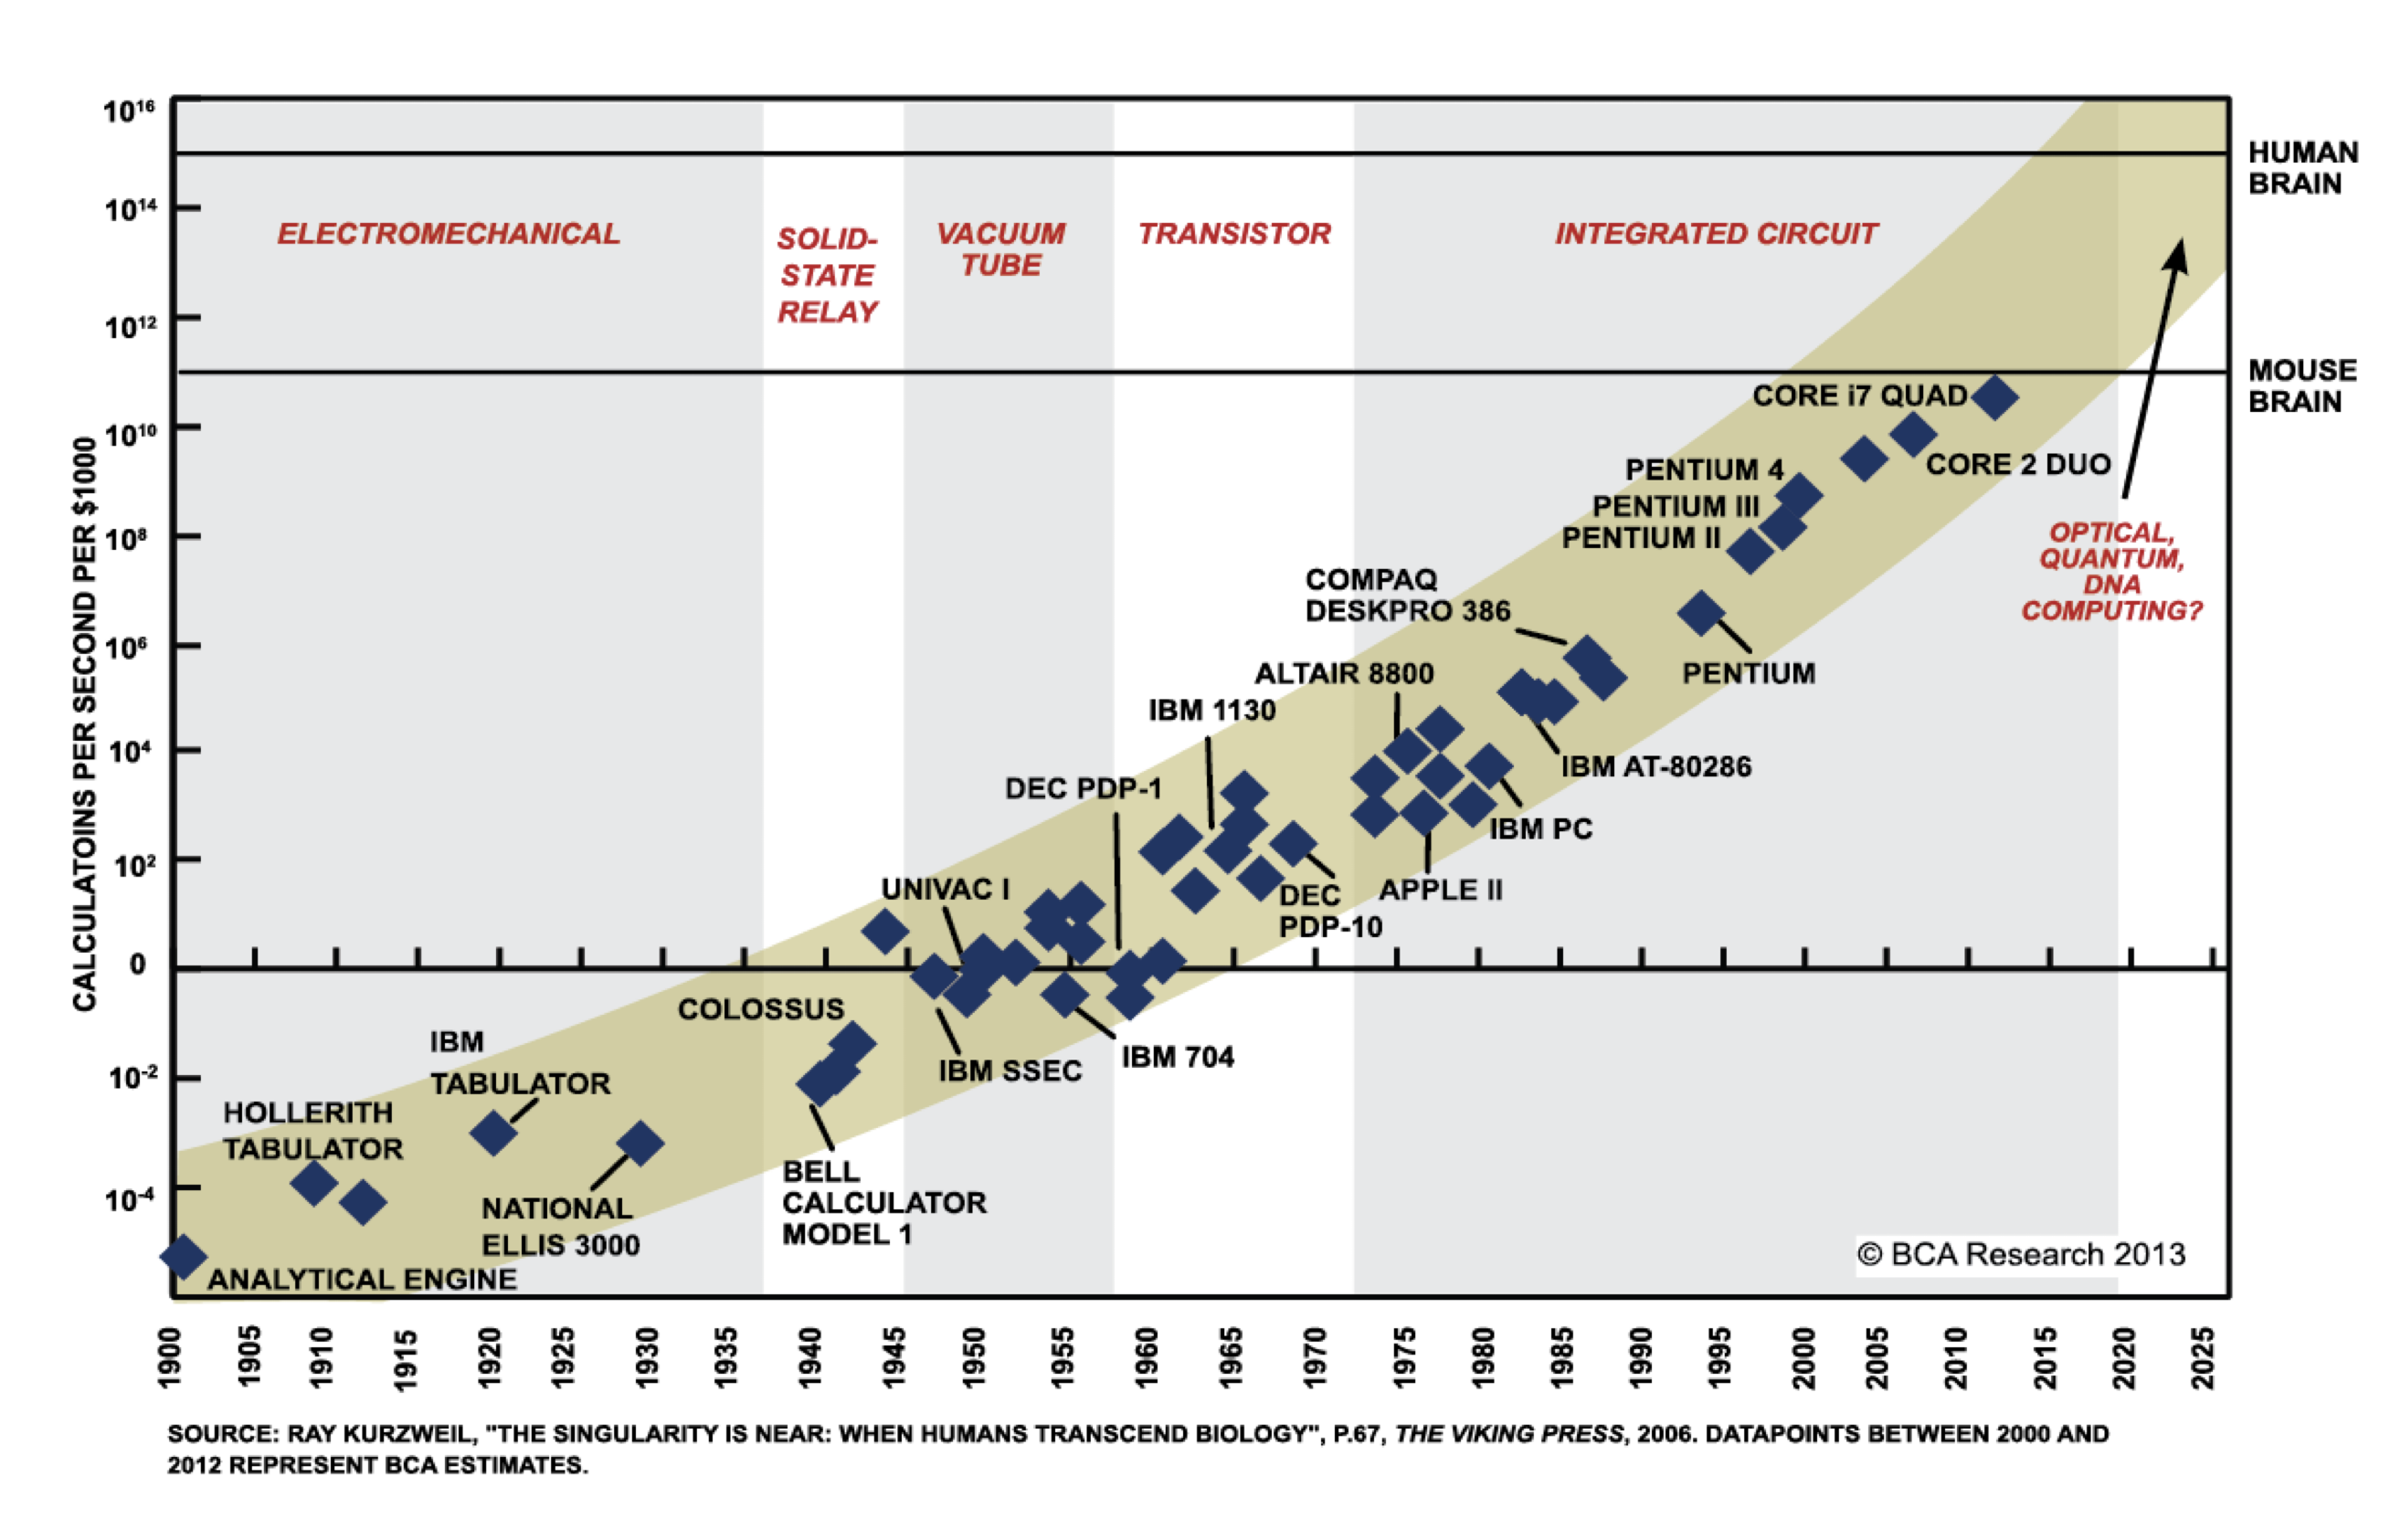
\includegraphics[width=0.65\linewidth]{figures/compute_cost.png}
%\end{figure}
%\end{frame}

%\begin{frame}{Additional Problems}
%\begin{itemize}
%\item Growing performance discrepancy between processing units and data storage
%\begin{itemize}
%\item 40\% processor performance improvement per year
%\item 10\% RAM performance improvement per year
%\end{itemize}
%\item Discrepancy leads to memory-bound programs
%\begin{itemize}
%\item CPU spends more and more time idle, waiting on data from
%\end{itemize}
%\item Many simulations require incredible amounts of memory to achieve high-accuracy solutions (PDE, MD, QM, etc.)
%\begin{itemize}
%\item These cannot fit on a single computer alone
%\end{itemize}
%\end{itemize}
%\end{frame}

%\begin{frame}{The Parallel Solution}
%\begin{itemize}
%\item Using multiple processing units (cores, etc.) simultaneously to perform a computation
%\item Use multiple computers to store data for large problems
%\item Essentially all modern CPUs have multiple cores
%\end{itemize}
%\end{frame}

\begin{frame}{Parallel Programming}
\centering
``I know how to make 4 horses pull a cart - I don't know how to make 1024
chickens do it.''\\Enrico Clementi
\end{frame}

\begin{frame}{What is High-Performance Computing}
\centering
High performance computing (HPC) is the use of computing resources that are
significantly more powerful than what is commonly available.

As such, it's always a moving target.
\end{frame}

%\begin{frame}{Supercomputer Types}
%\begin{columns}
%\begin{column}{0.5\textwidth}
%\begin{itemize}
%\item Single processor
%\item Shared Memory Parallel (SMP)
%\item Massively Parallel Processors
%\item Constellations
%\item Clusters
%\end{itemize}
%\end{column}
%\begin{column}{0.5\textwidth}
%\begin{center}
%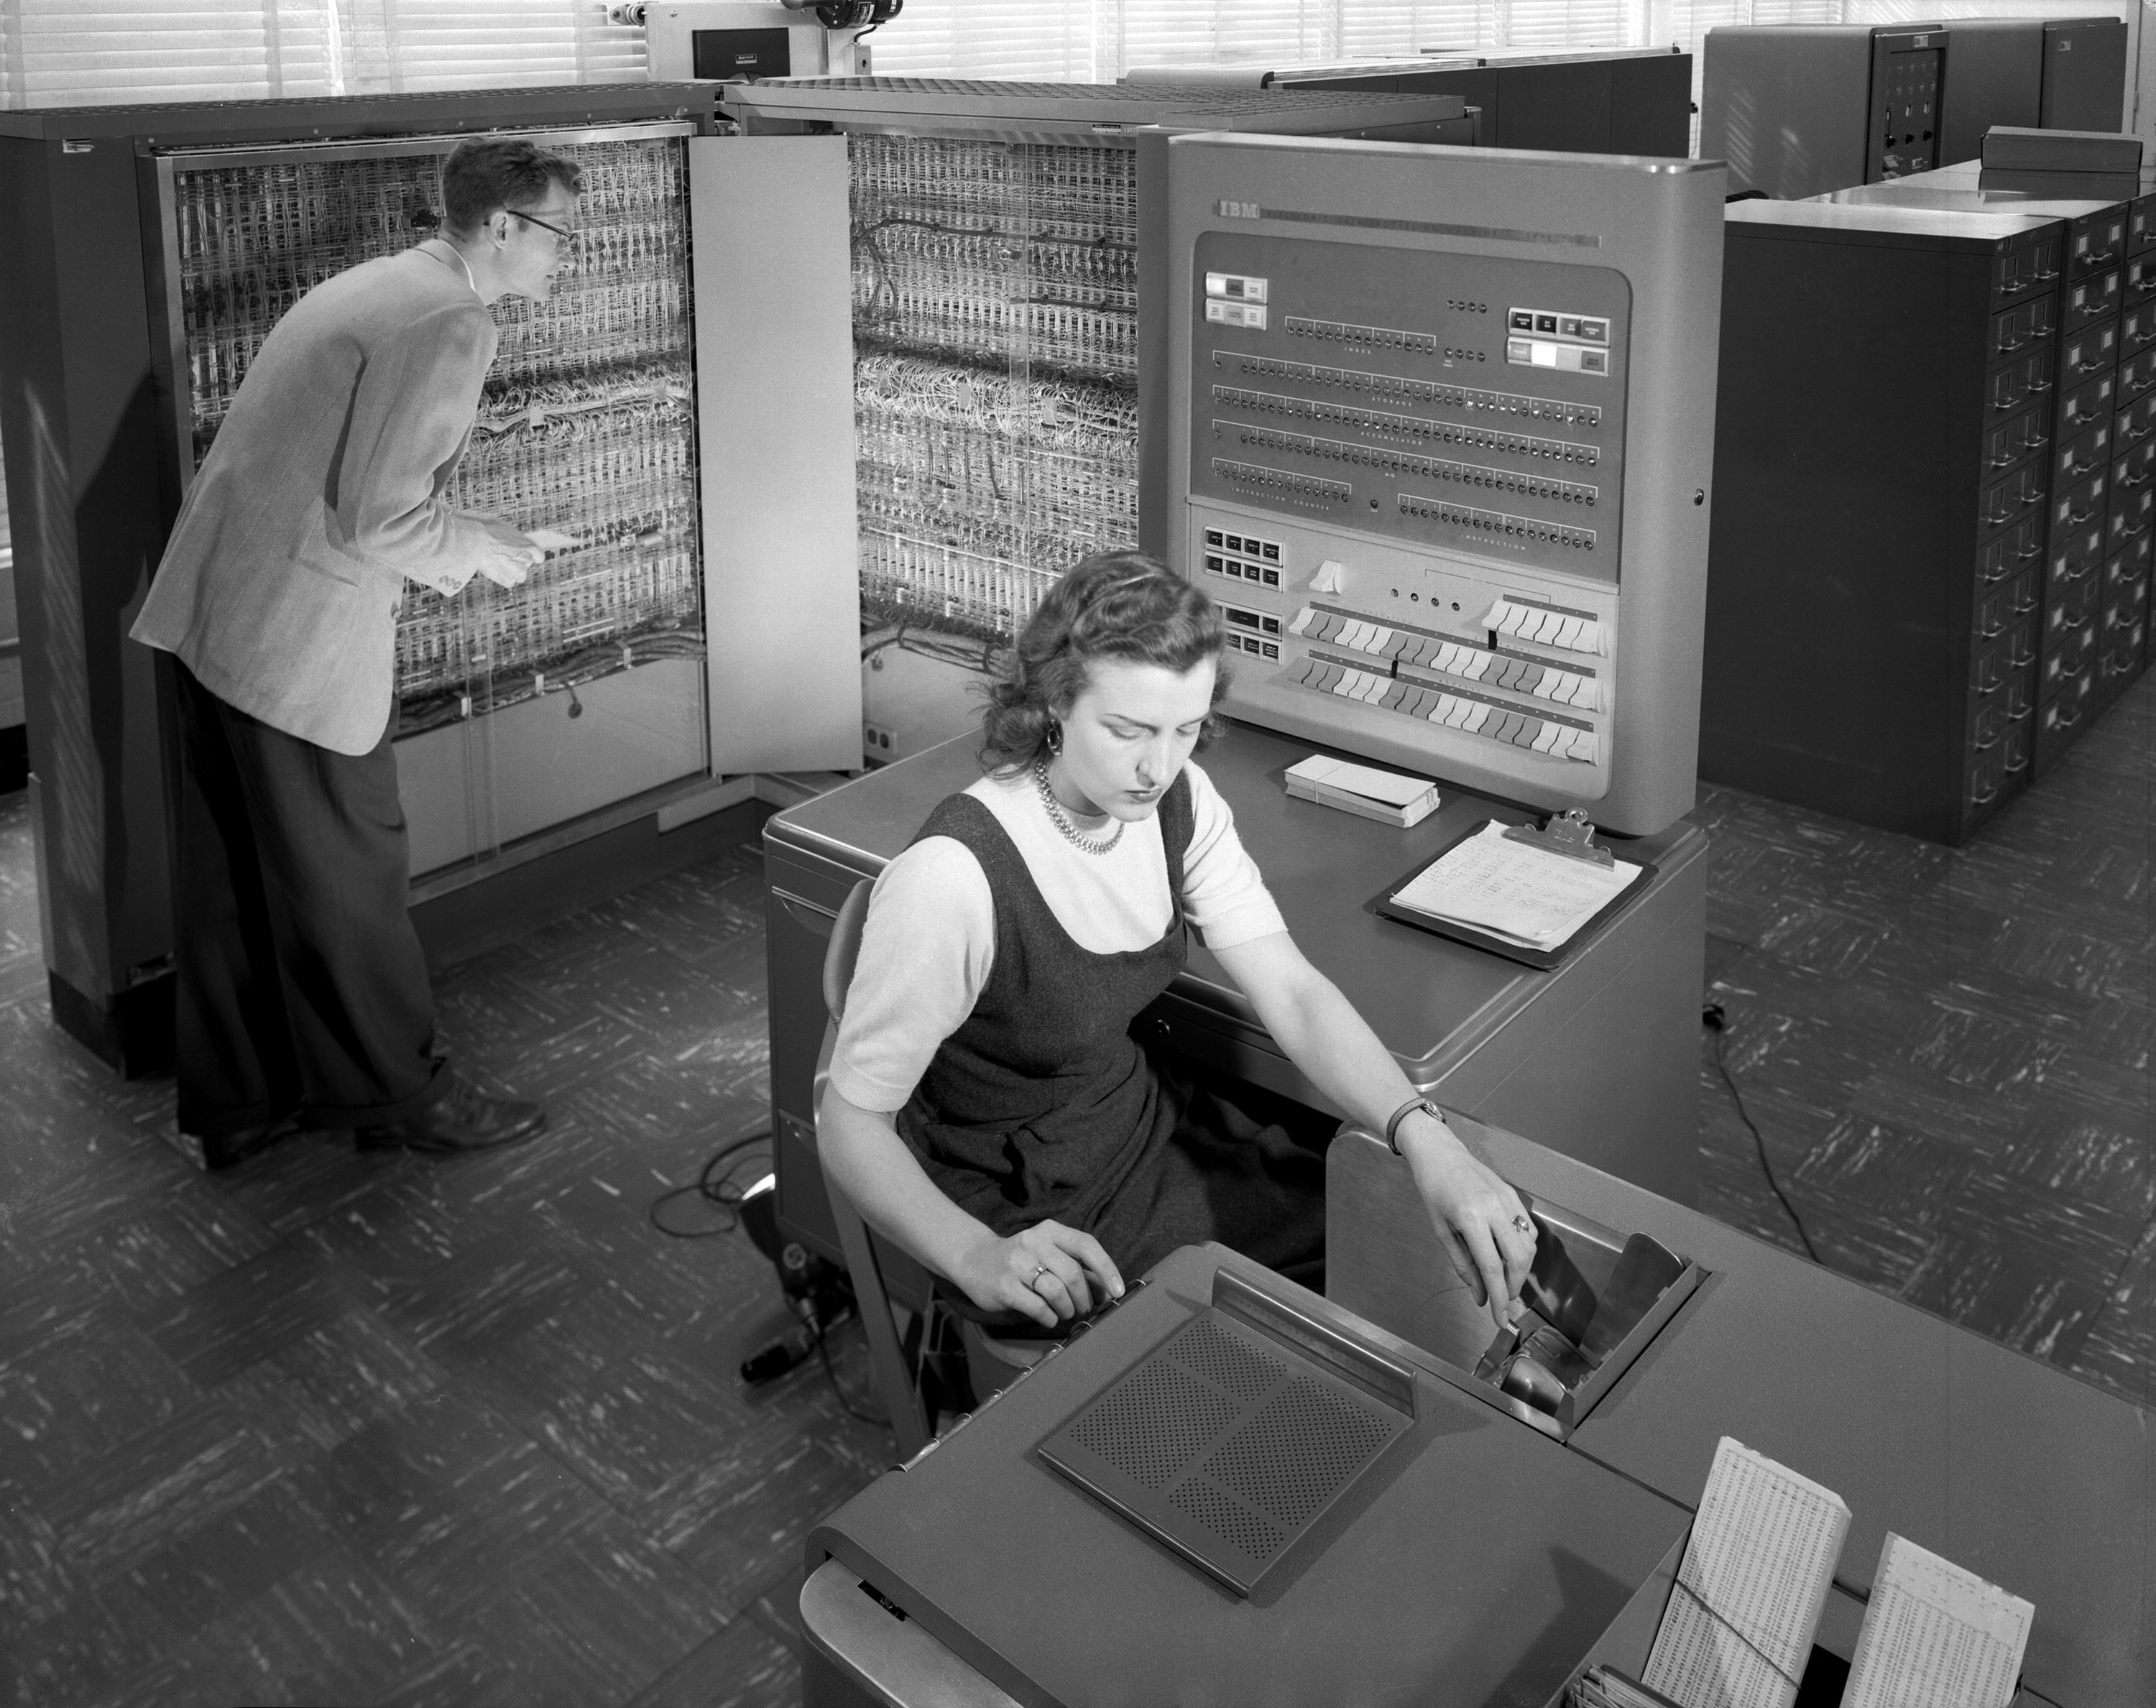
\includegraphics[width=\textwidth]{figures/mainframe.jpg}
%\end{center}
%\end{column}
%\end{columns}
%\end{frame}
%
%\begin{frame}{History of Parallel Architectures}
%\begin{columns}
%\begin{column}{0.5\textwidth}
%\begin{center}
%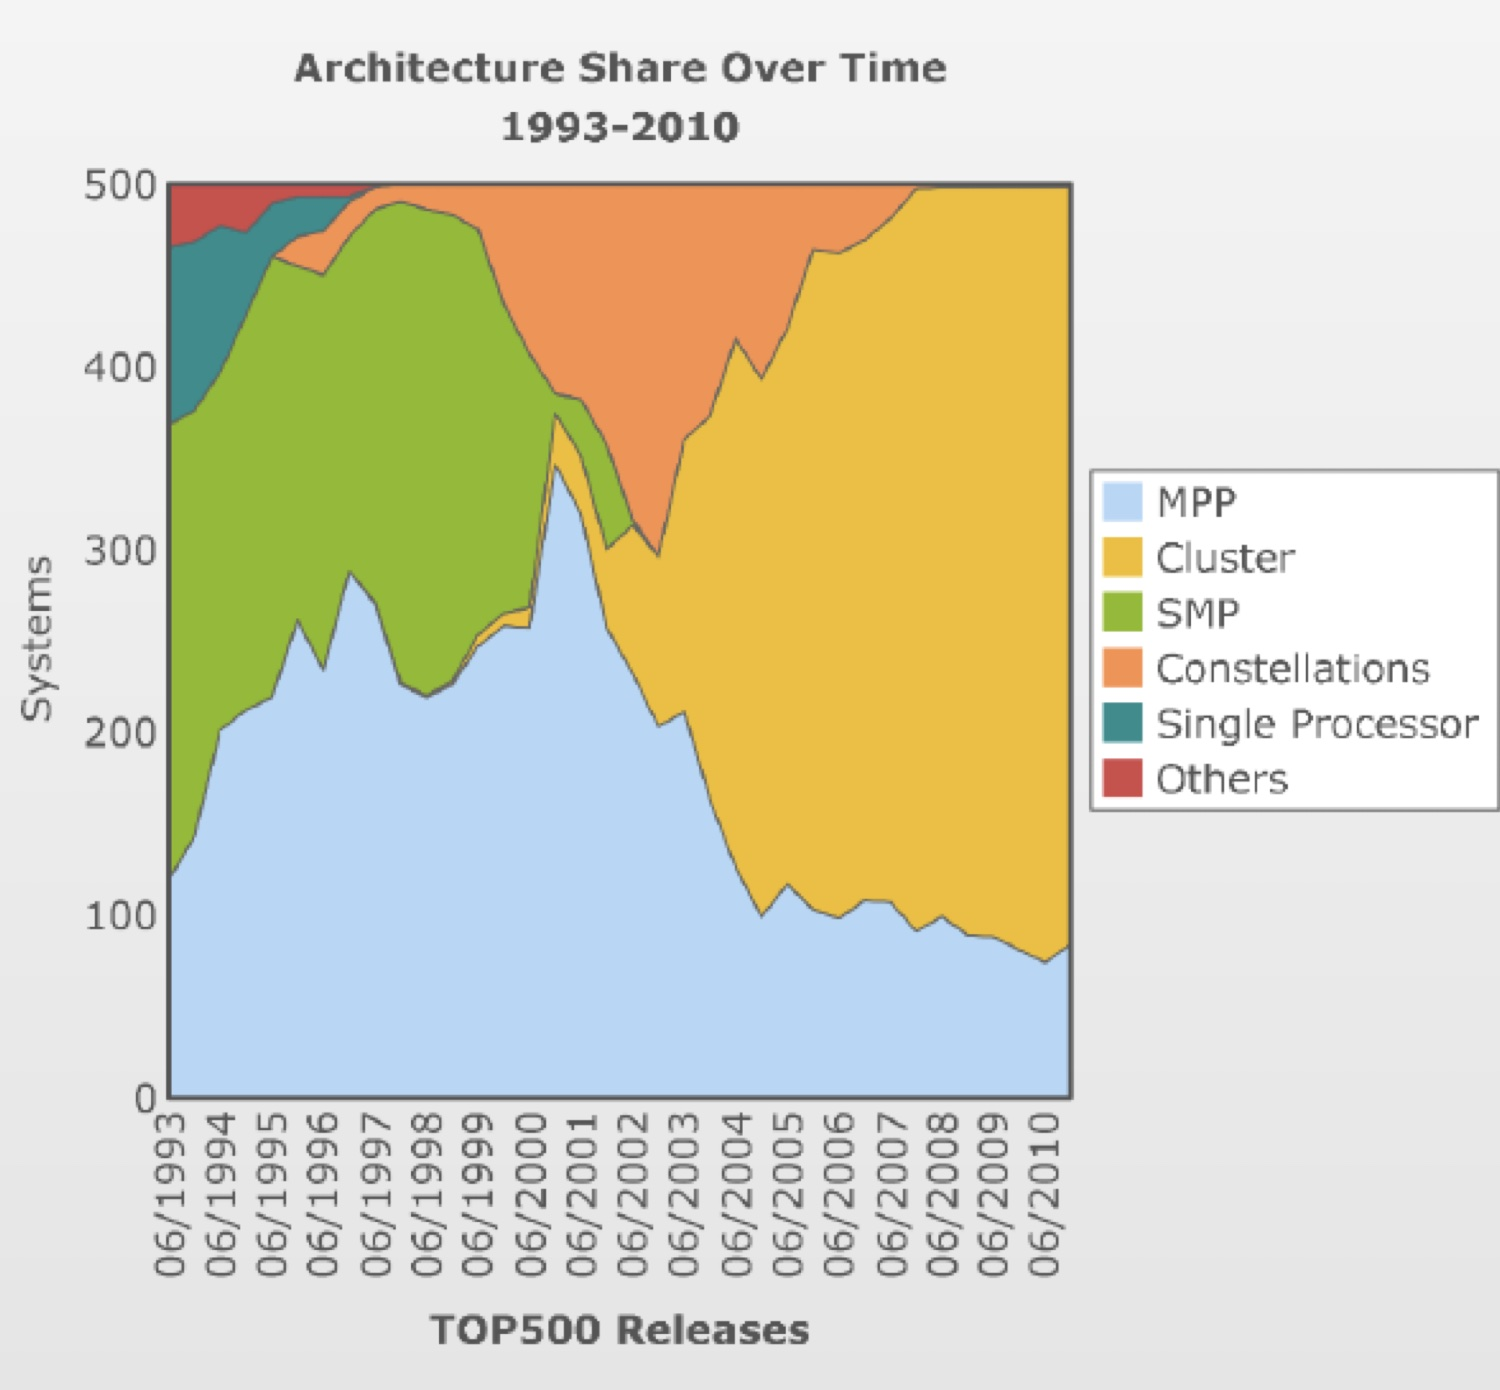
\includegraphics[width=\textwidth]{figures/top500_architecture.jpg}
%\end{center}
%\end{column}
%\begin{column}{0.5\textwidth}
%\begin{center}
%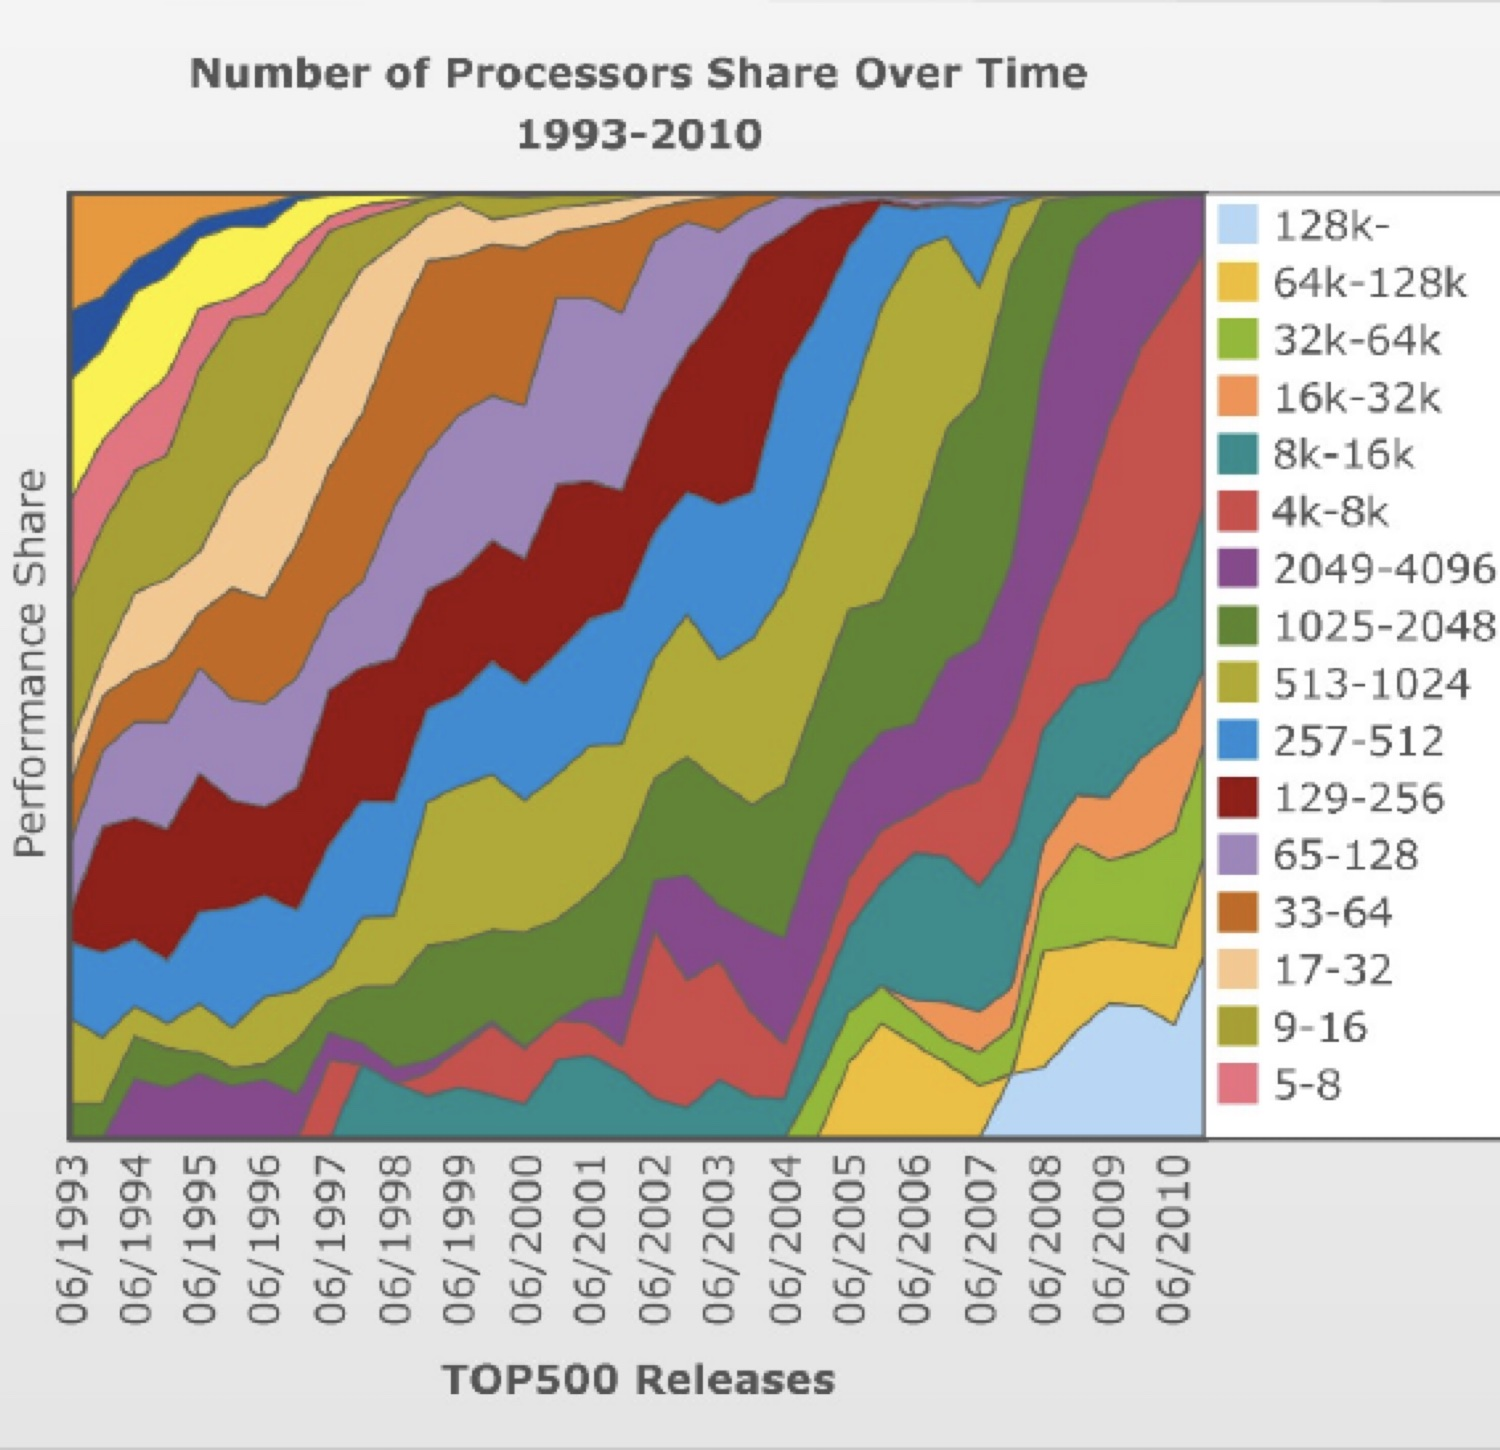
\includegraphics[width=\textwidth]{figures/top500_core_count.jpg}
%\end{center}
%\end{column}
%\end{columns}
%\end{frame}
%
%\begin{frame}{Flynn’s Parallel Architecture Taxonomy}
%\begin{columns}
%\begin{column}{0.5\textwidth}
%\begin{itemize}
%\item Single/multiple instruction streams
%\begin{itemize}
%\item Number of types of instructions to be performed at once
%\end{itemize}
%\item Single/multiple data streams
%\begin{itemize}
%\item Number of data streams to be operated on at once
%\end{itemize}
%\item Most modern parallel computers are MIMD
%\item SIMD was popular until 1990s
%\item MISD never used to large extent
%\end{itemize}
%\end{column}
%\begin{column}{0.5\textwidth}
%\begin{center}
%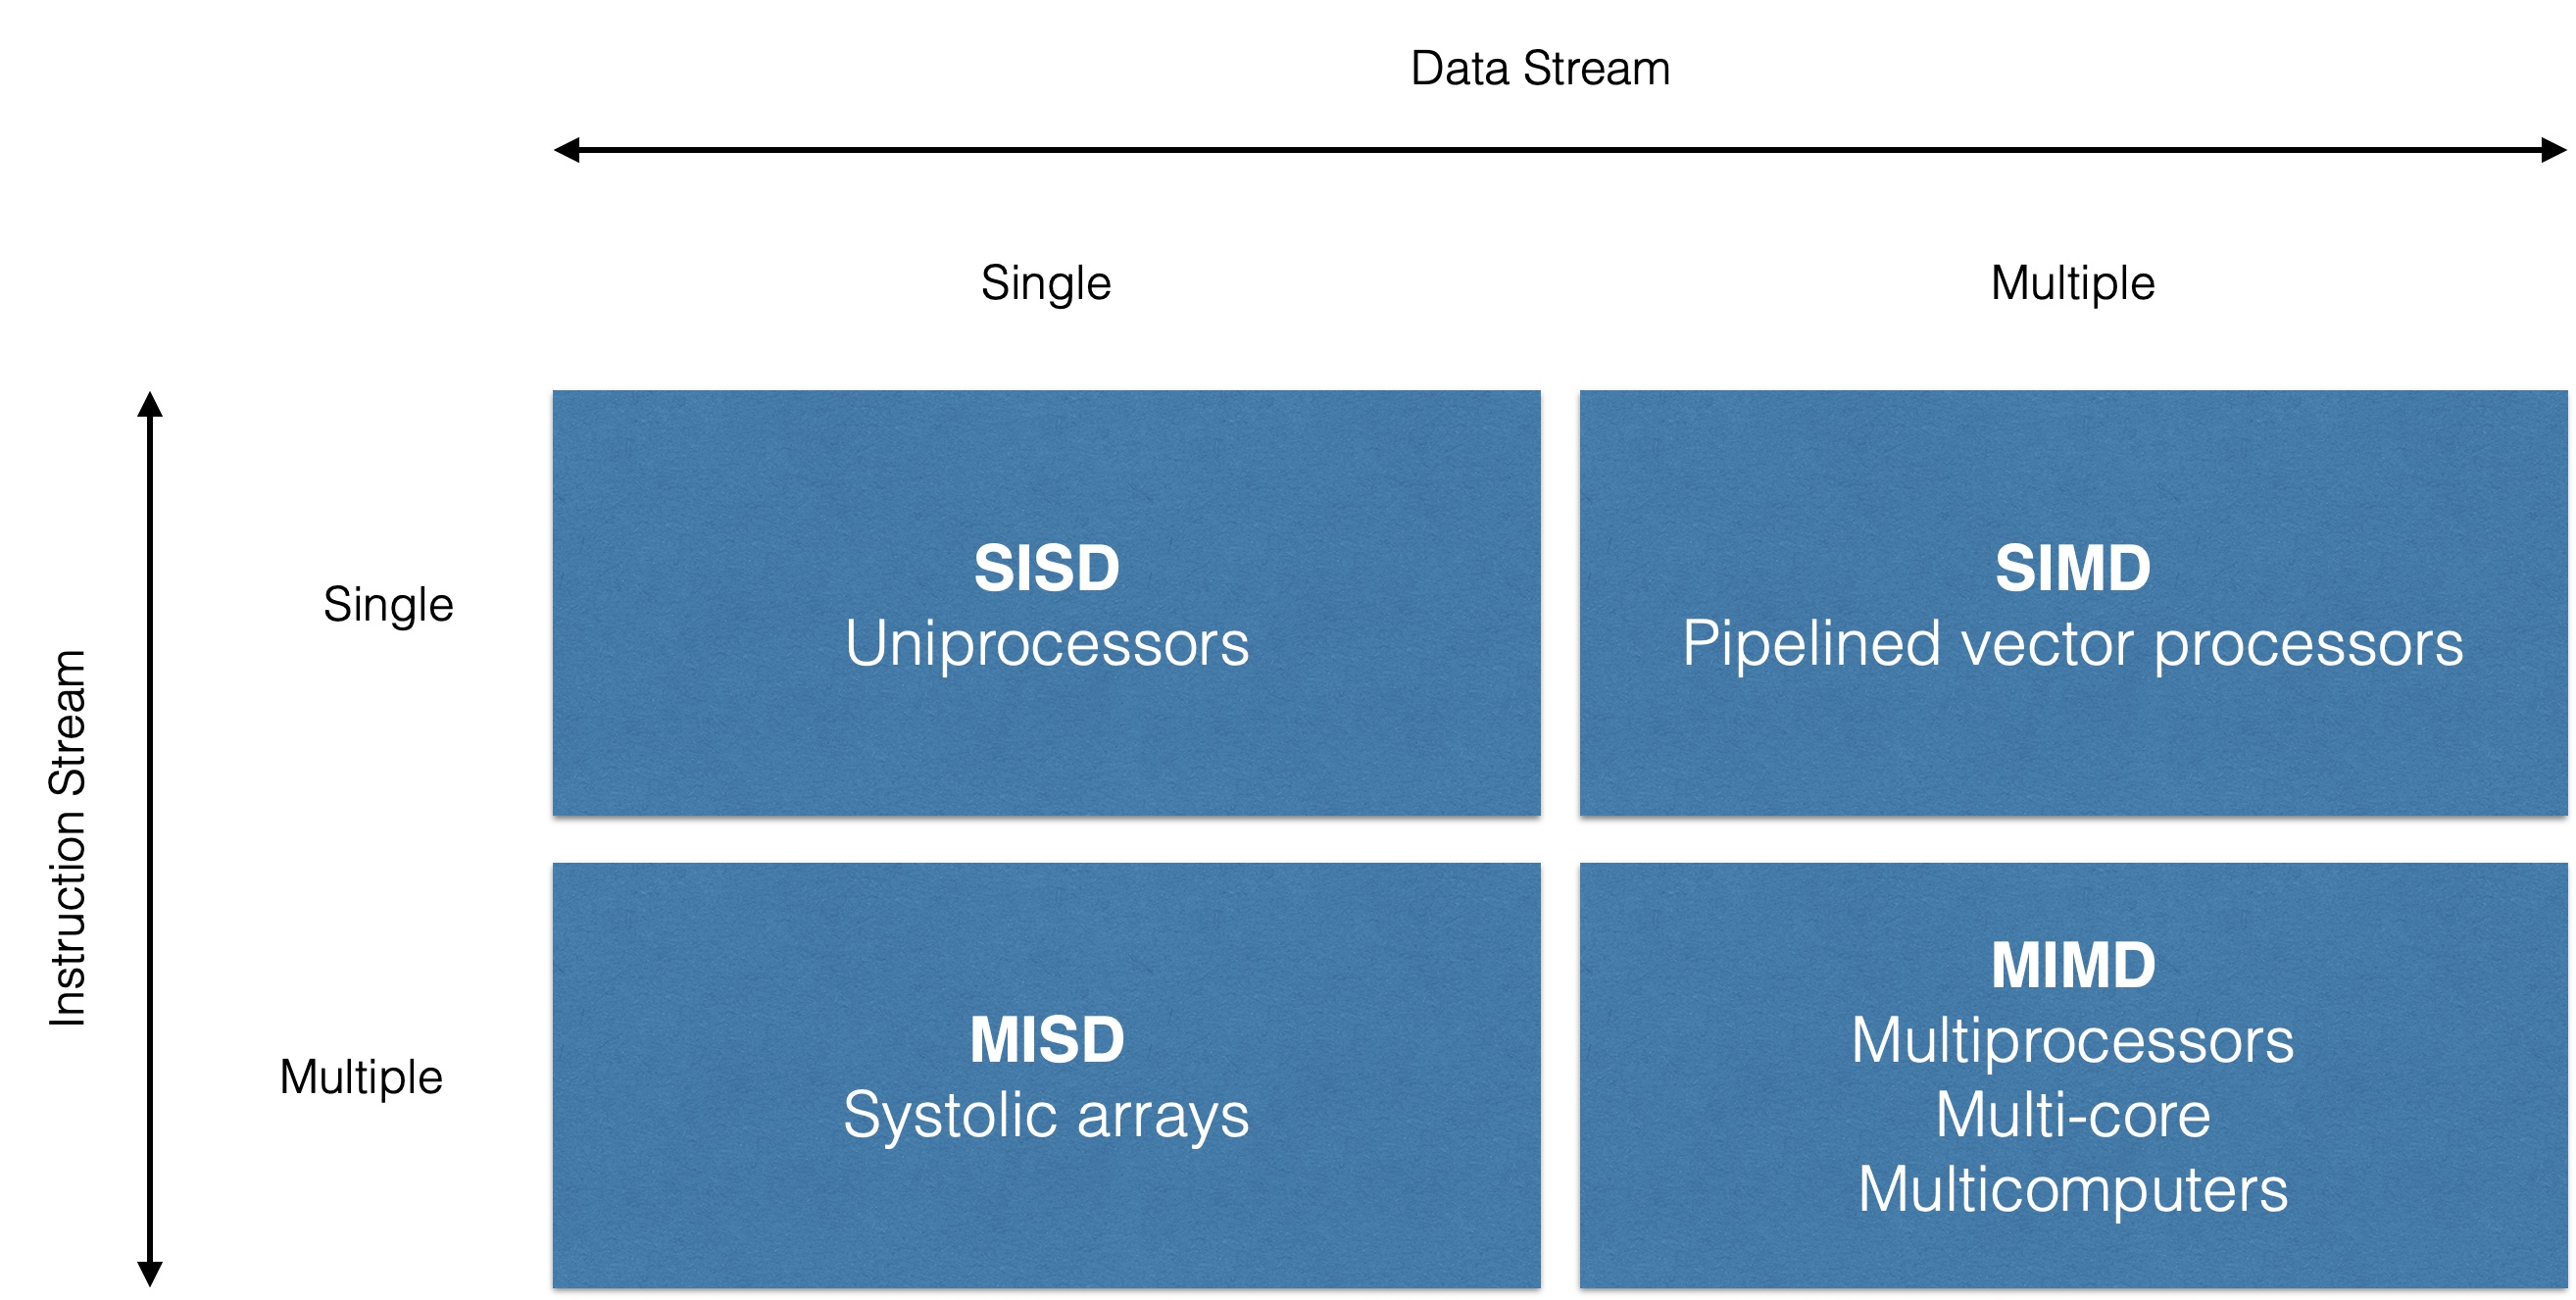
\includegraphics[width=\textwidth]{figures/flynn_taxonomy.jpg}
%\end{center}
%\end{column}
%\end{columns}
%\end{frame}
%
%\begin{frame}{Multicomputer Architecture}
%\begin{center}
%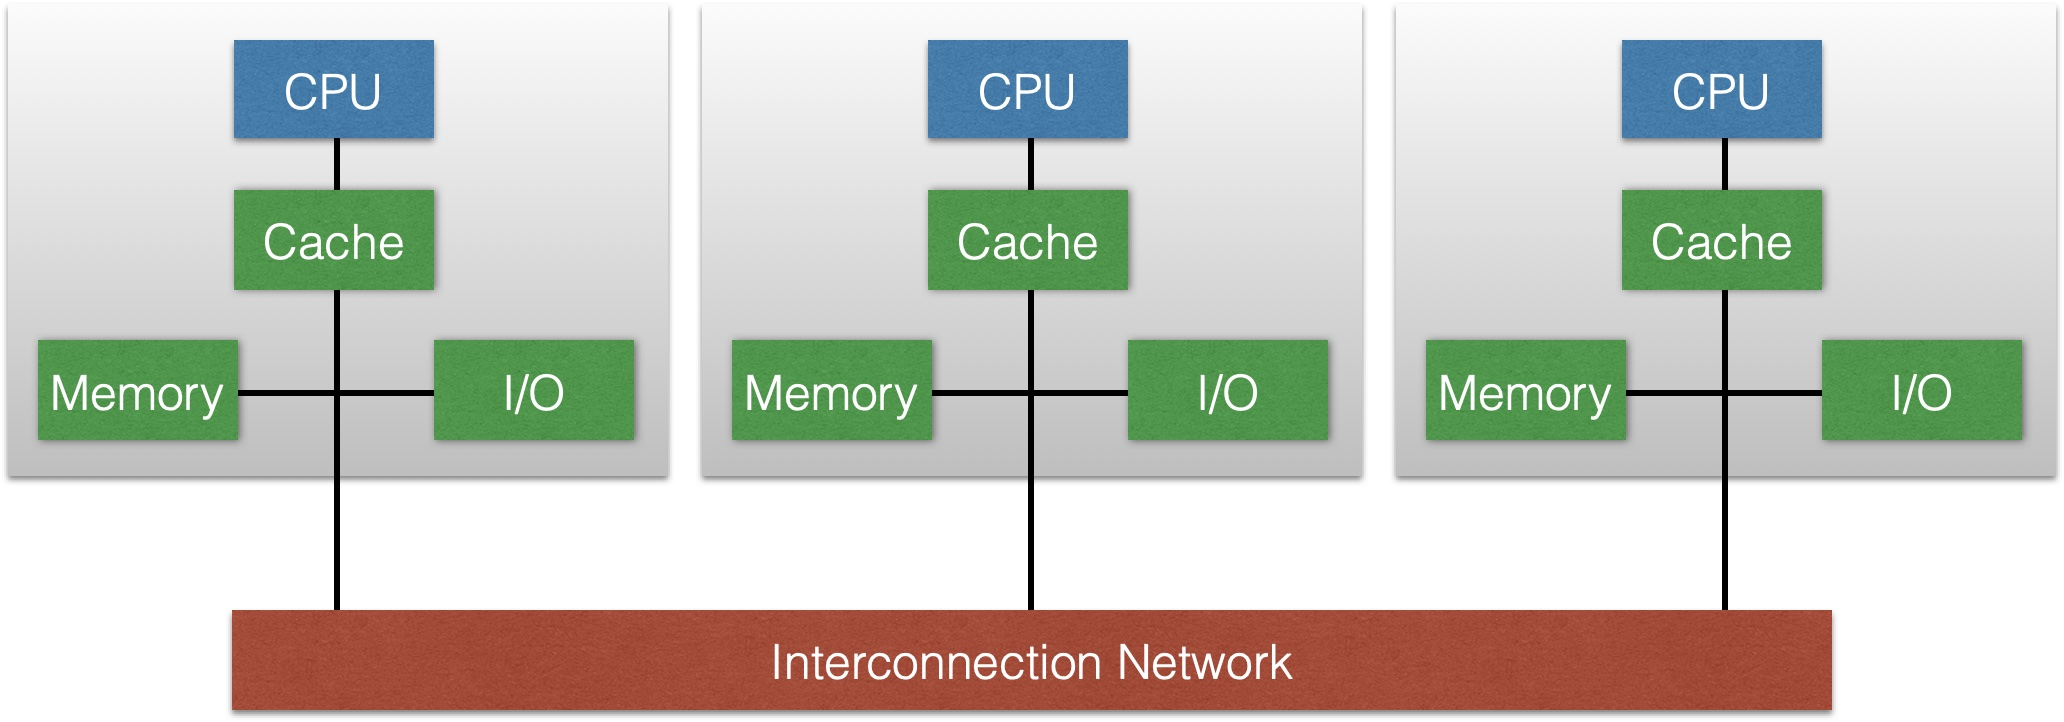
\includegraphics[scale=0.25]{figures/cluster_interconnect.jpg}
%\end{center}
%\begin{itemize}
%\item Each processor only has direct access to its own local memory address space
%\begin{itemize}
%\item The same address on different processors refers to different memory locations
%\end{itemize}
%\item Processors interact with one another through passing messages
%\item Commercial multicomputers typically provide a custom switching network to
%      provide low-latency, high-bandwidth access between processors
%\end{itemize}
%\end{frame}
%
%\begin{frame}{Multicomputer Architecture}
%\begin{itemize}
%\item Commodity clusters are build using commodity computers and switches/LANs
%\item Less costly than SMP's
%\item Increased latency/decreased bandwidth between CPUs
%\item Theoretically extensible to arbitrary processor counts
%\item Software becomes complicated
%\item Networking gets expensive
%\end{itemize}
%\end{frame}
%
%\begin{frame}{Cluster Storage Resources}
%\begin{columns}
%\begin{column}{0.5\textwidth}
%\begin{itemize}
%\item Usually there is an inverse relationship between storage amount and speed
%\item Clusters and applications can distort the standard order
%\begin{itemize}
%\item Aggregation, e.g. RAID
%\item Network optimization to a specific topology
%\item Applications can be configured and built for specific hardware
%\item New hardware technologies
%\end{itemize}
%\end{itemize}
%\end{column}
%\begin{column}{0.5\textwidth}
%\begin{center}
%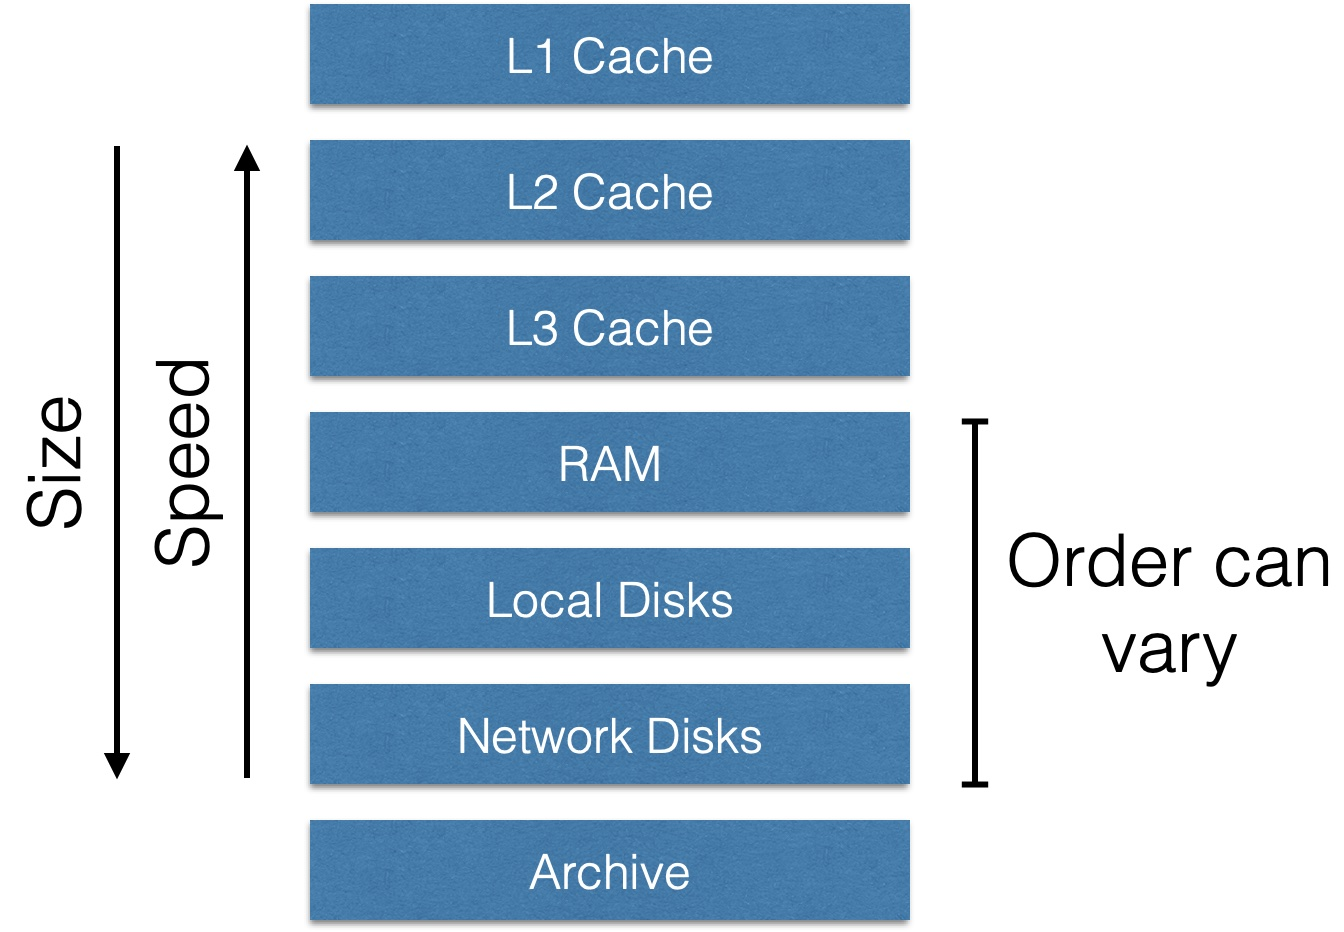
\includegraphics[width=\textwidth]{figures/storage_hierarchy.jpg}
%\end{center}
%\end{column}
%\end{columns}
%\end{frame}

\begin{frame}{Cluster Super Computers}
\begin{figure}
  \centering
  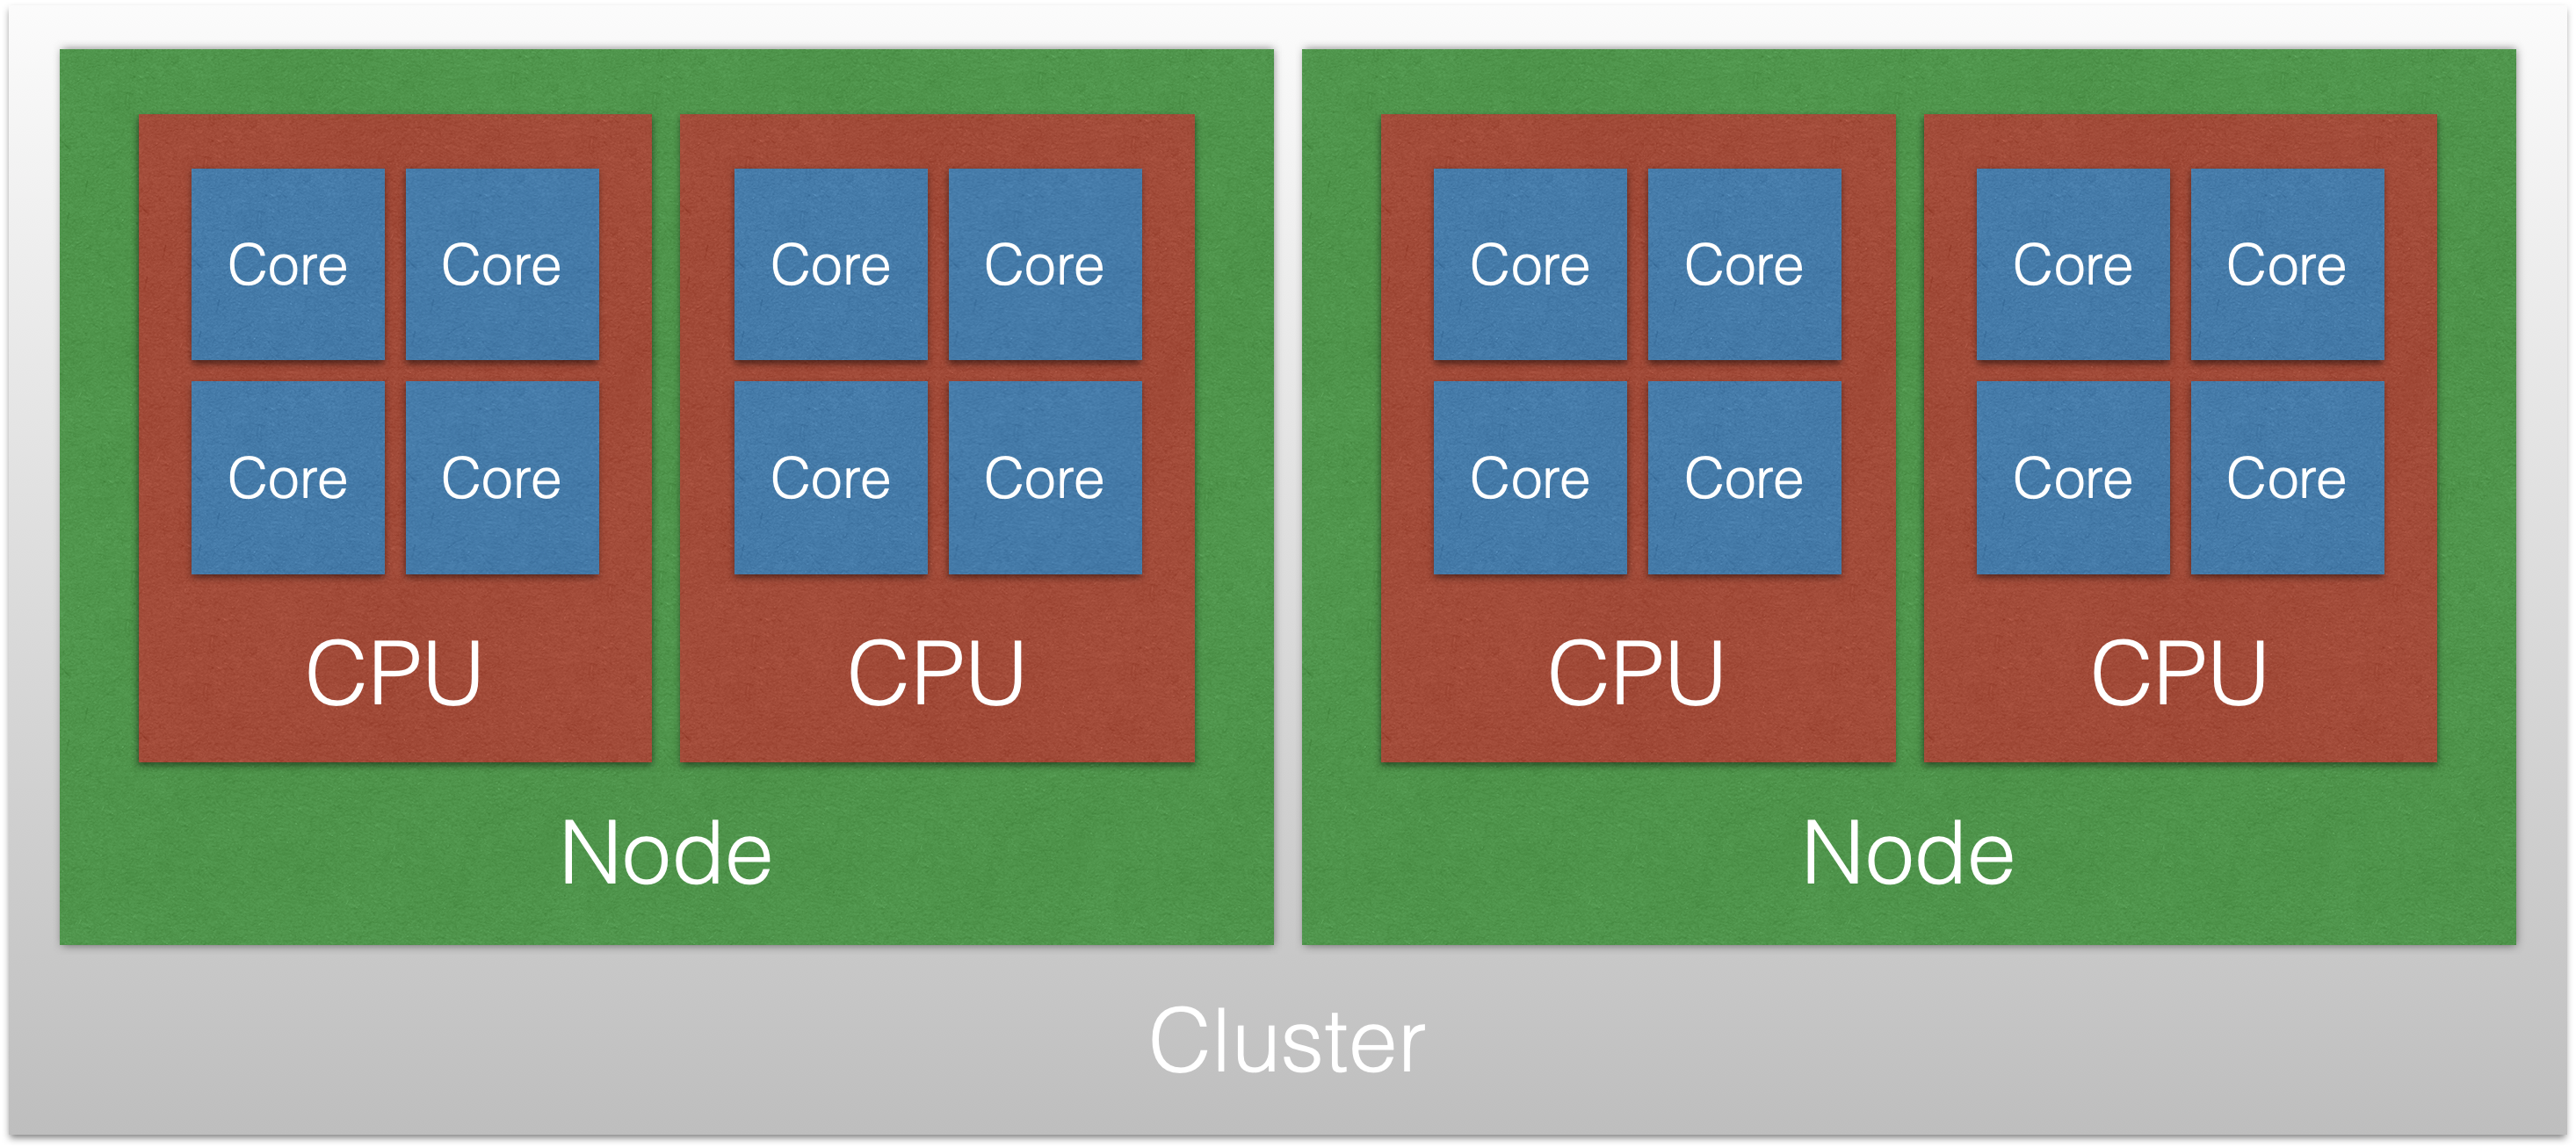
\includegraphics[width=0.75\linewidth]{figures/cluster.png}
  \caption{A cluster is a collection of individual computers networked together. Applications can be configured to run on all available compute resources.}
\end{figure}
\end{frame}

\section{SMU HPC Clusters}

\begin{frame}{SMU HPC Clusters}
\begin{table}
\scriptsize
\begin{tabular}{llllll}
\toprule
HPC System & M1 & M2 & M2 & SuperPOD & M3 \\
\midrule
Year & 2014 & 2017 & 2019 & 2022 & 2023 \\
Compute Ability & 104 TFLOPS & 630 TFLOPS & 870 TFLOPS & 1,644 TFLOPS &
1,003 TFLOPS \\
Number of Nodes & 1,104 & 349 & 354 & 20 & 178 \\
CPU Cores & 8,832 & 11,088 & 11,276 & 2,560 & 22,784 \\
Total GPU Cores & 0 & 132,608 & 275,968 & 1,392,640 & 0 \\
Total Memory & 29.2 TB & 116.5 TB & 120 TB & 52.5 TB & 101 TB \\
Network Bandwidth & 20 Gb/s & 100 Gb/s & 100 Gb/s & 200 Gb/s & 200
Gb/s \\
Work Storage & None & None & 768 TB & 768 TB & 3.5 PB \\
Scratch Space & 1.4 PB & 1.4 PB & 2.8 PB & 750 TB & 3.5 PB \\
Archive Capabilities & No & Yes & Yes & No & No \\
Operating System & Scientific Linux 6 & CentOS 7 & CentOS 7 & Ubuntu
20.04 & Ubuntu 22.04 \\
\bottomrule
\end{tabular}
\end{table}
\end{frame}

\begin{frame}{M3 Node Configuration}
\begin{table}
\begin{tabular}{lll}
\toprule
Resource & Standard-Memory & High-Memory \\
\midrule
Nodes & 170 & 8 \\
Processors & AMD EPYC 7763 & AMD EPYC 7763 \\
Frequency & 2.45 GHz & 2.45 GHz \\
CPUs/Node & 2 & 2 \\
Cores/Node & 128 & 128 \\
Memory/Node & 512 GB & 2 TB \\
Local Scratch/Node & None & 4.3 TB \\
Interconnect & 200 Gb/s & 200 Gb/s \\
\bottomrule
\end{tabular}
\end{table}
\end{frame}

\begin{frame}{NVIDIA DGX SuperPOD (MP)}
\begin{columns}
\begin{column}{0.5\textwidth}
\begin{table}
\tiny
\begin{tabular}{ll}
\toprule
Component & Summary \\
\midrule
Computational Ability & 1,644 TFLOPS \\
Number of Nodes & 20 \\
CPU Cores & 2,560 \\
GPU Accelerator Cores & 1,392,640 \\
Total Memory & 52.5 TB \\
Interconnect Bandwidth & 10x200 Gb/s Infiniband Connections Per Node \\
Work Storage & 768 TB (Shared) \\
Scratch Storage & 750 TB (Raw) \\
Operating System & Ubuntu 20.04 \\
\bottomrule
\end{tabular}
\end{table}
\end{column}
\begin{column}{0.5\textwidth}
\begin{center}
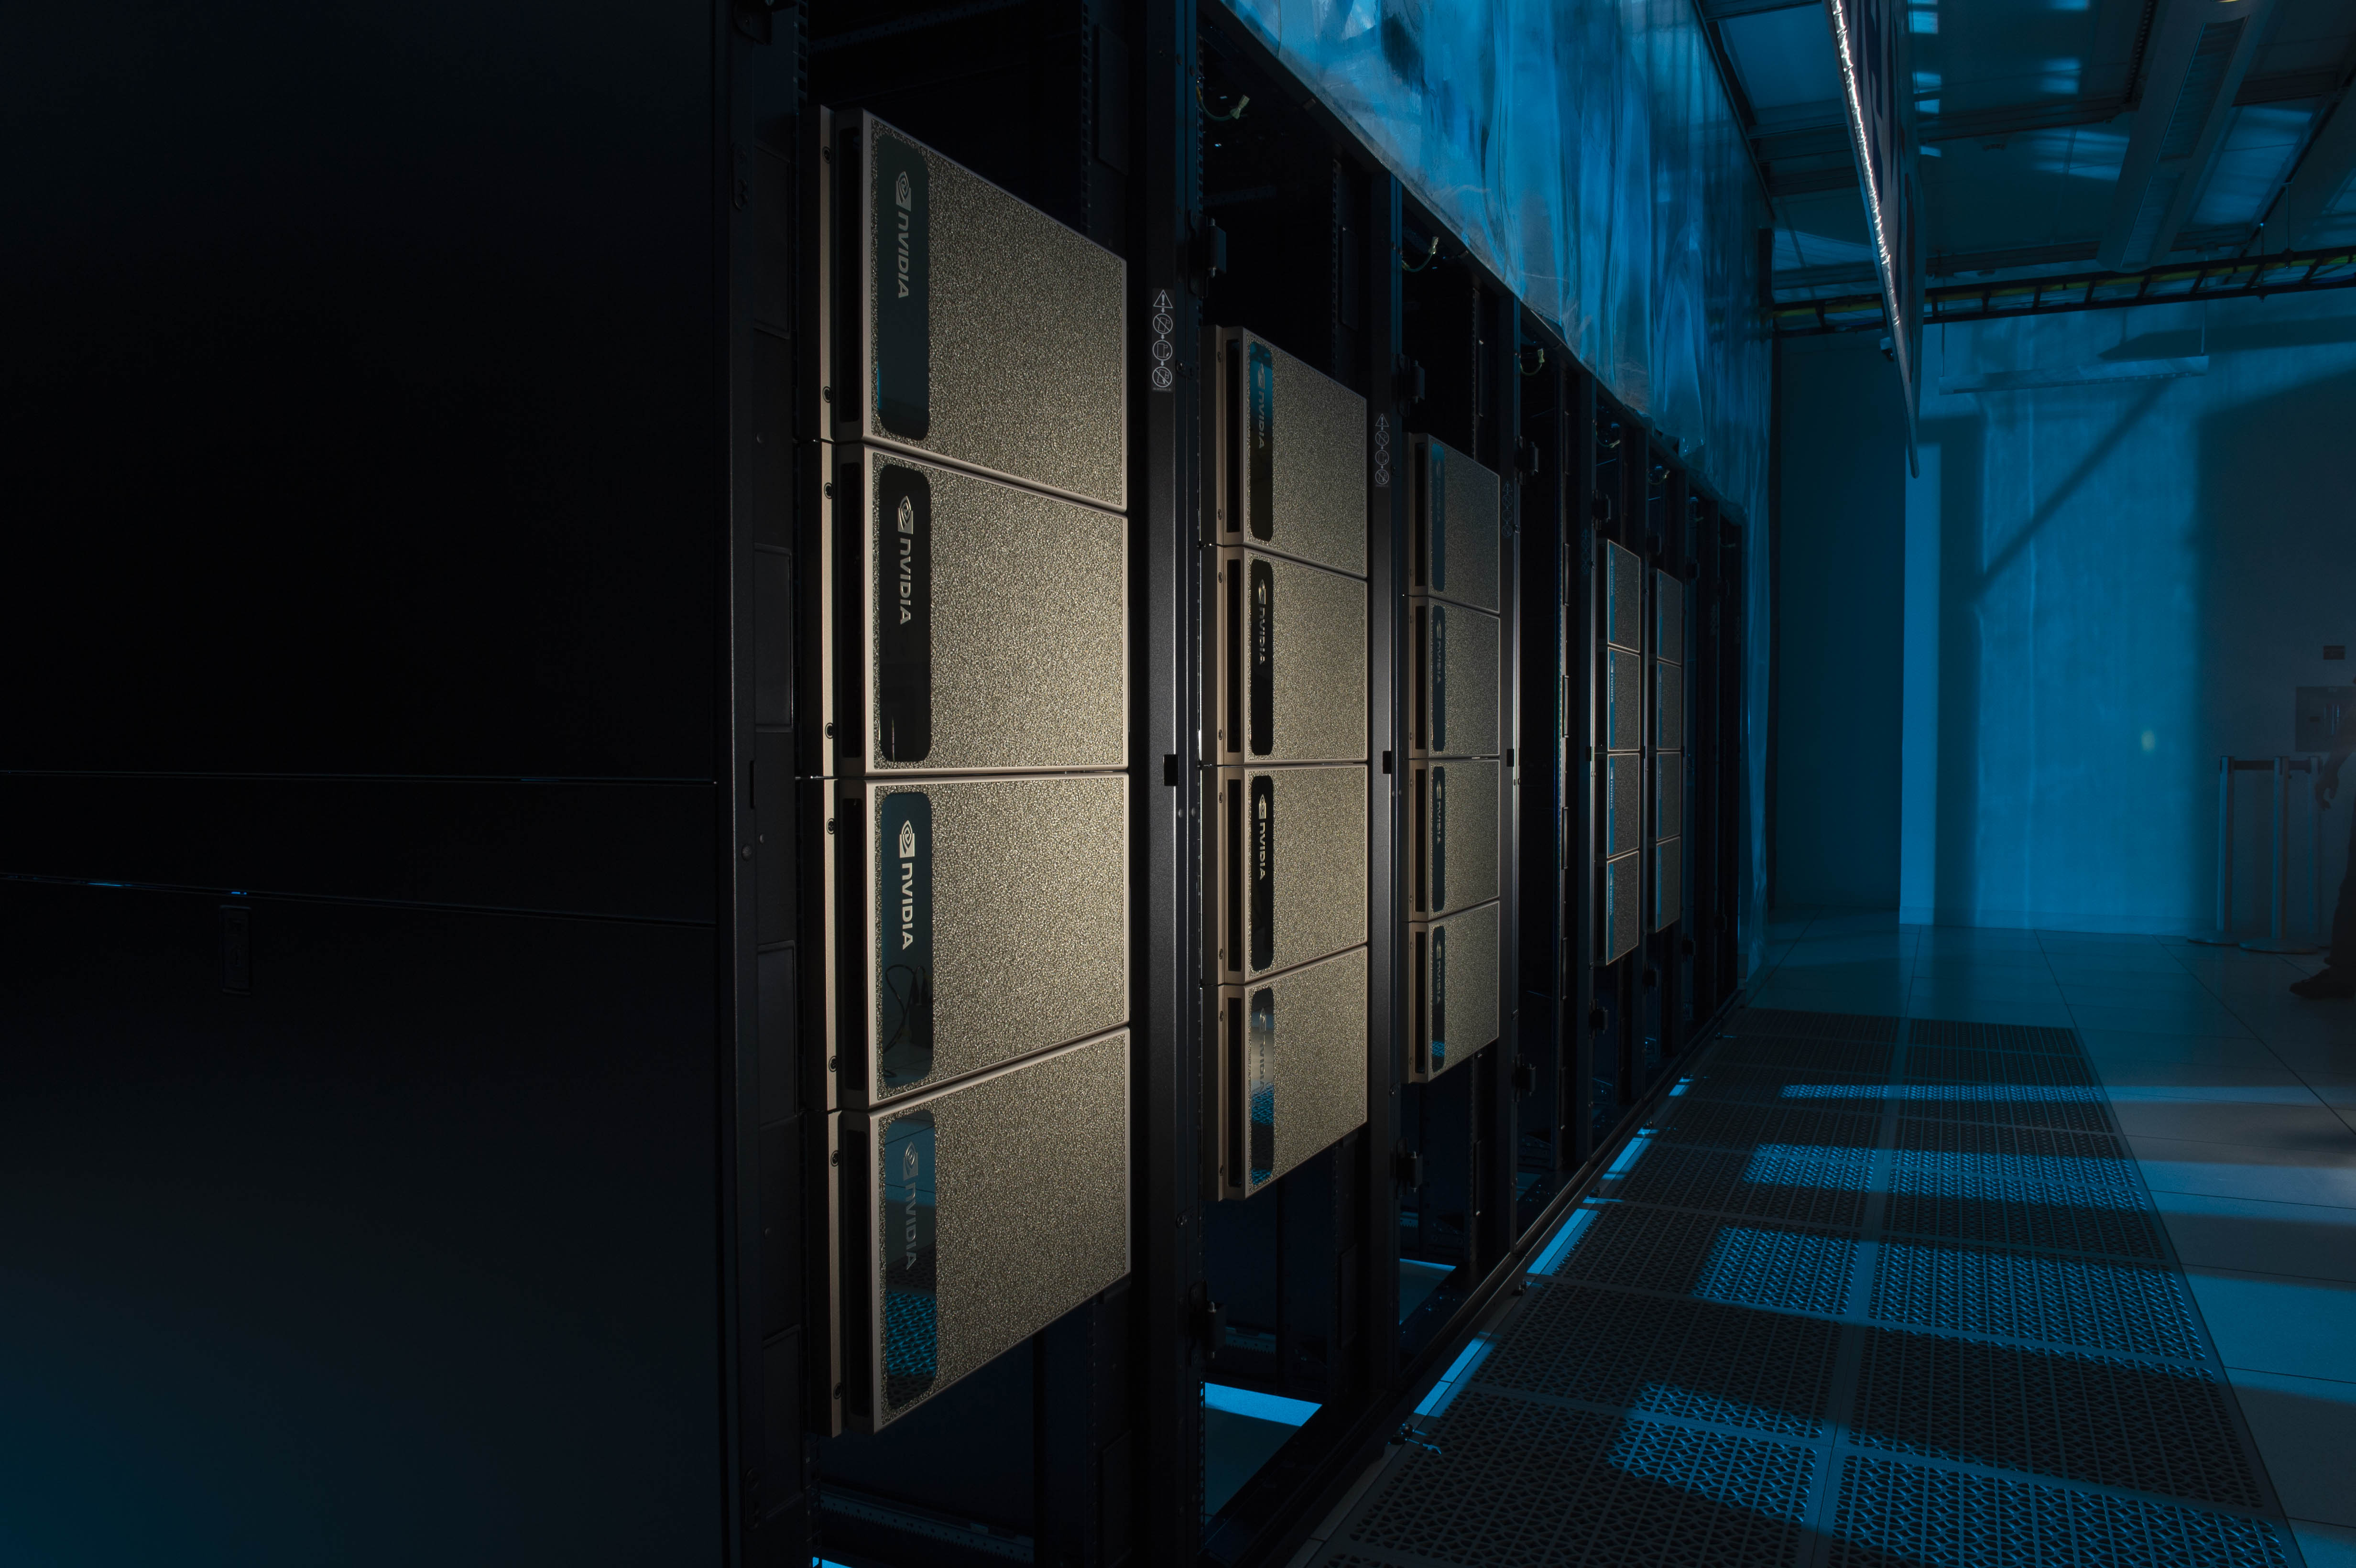
\includegraphics[width=\textwidth]{figures/superpod.jpg}
\end{center}
\end{column}
\end{columns}
\end{frame}

\begin{frame}{NVIDIA DGX Node Configuration}
\begin{columns}
\begin{column}{0.5\textwidth}
\begin{table}
\tiny
\begin{tabular}{ll}
\toprule
Resource & DGX Node \\
\midrule
Processors & AMD EPYC 7742 \\
CPUs/Node & 2 \\
Cores/Node & 128 \\
Memory/Node & 2 TB \\
GPUs & NVIDIA A100 Tensor Core GPU \\
GPUs/Node & 8 \\
GPU Memory/GPU & 80 GB \\
GPU Interconnect & NVLink \\
Local Scratch/Node & 27 TB \\
Network & 10x200 Gb/s \\
\bottomrule
\end{tabular}
\end{table}
\end{column}
\begin{column}{0.5\textwidth}
\begin{center}
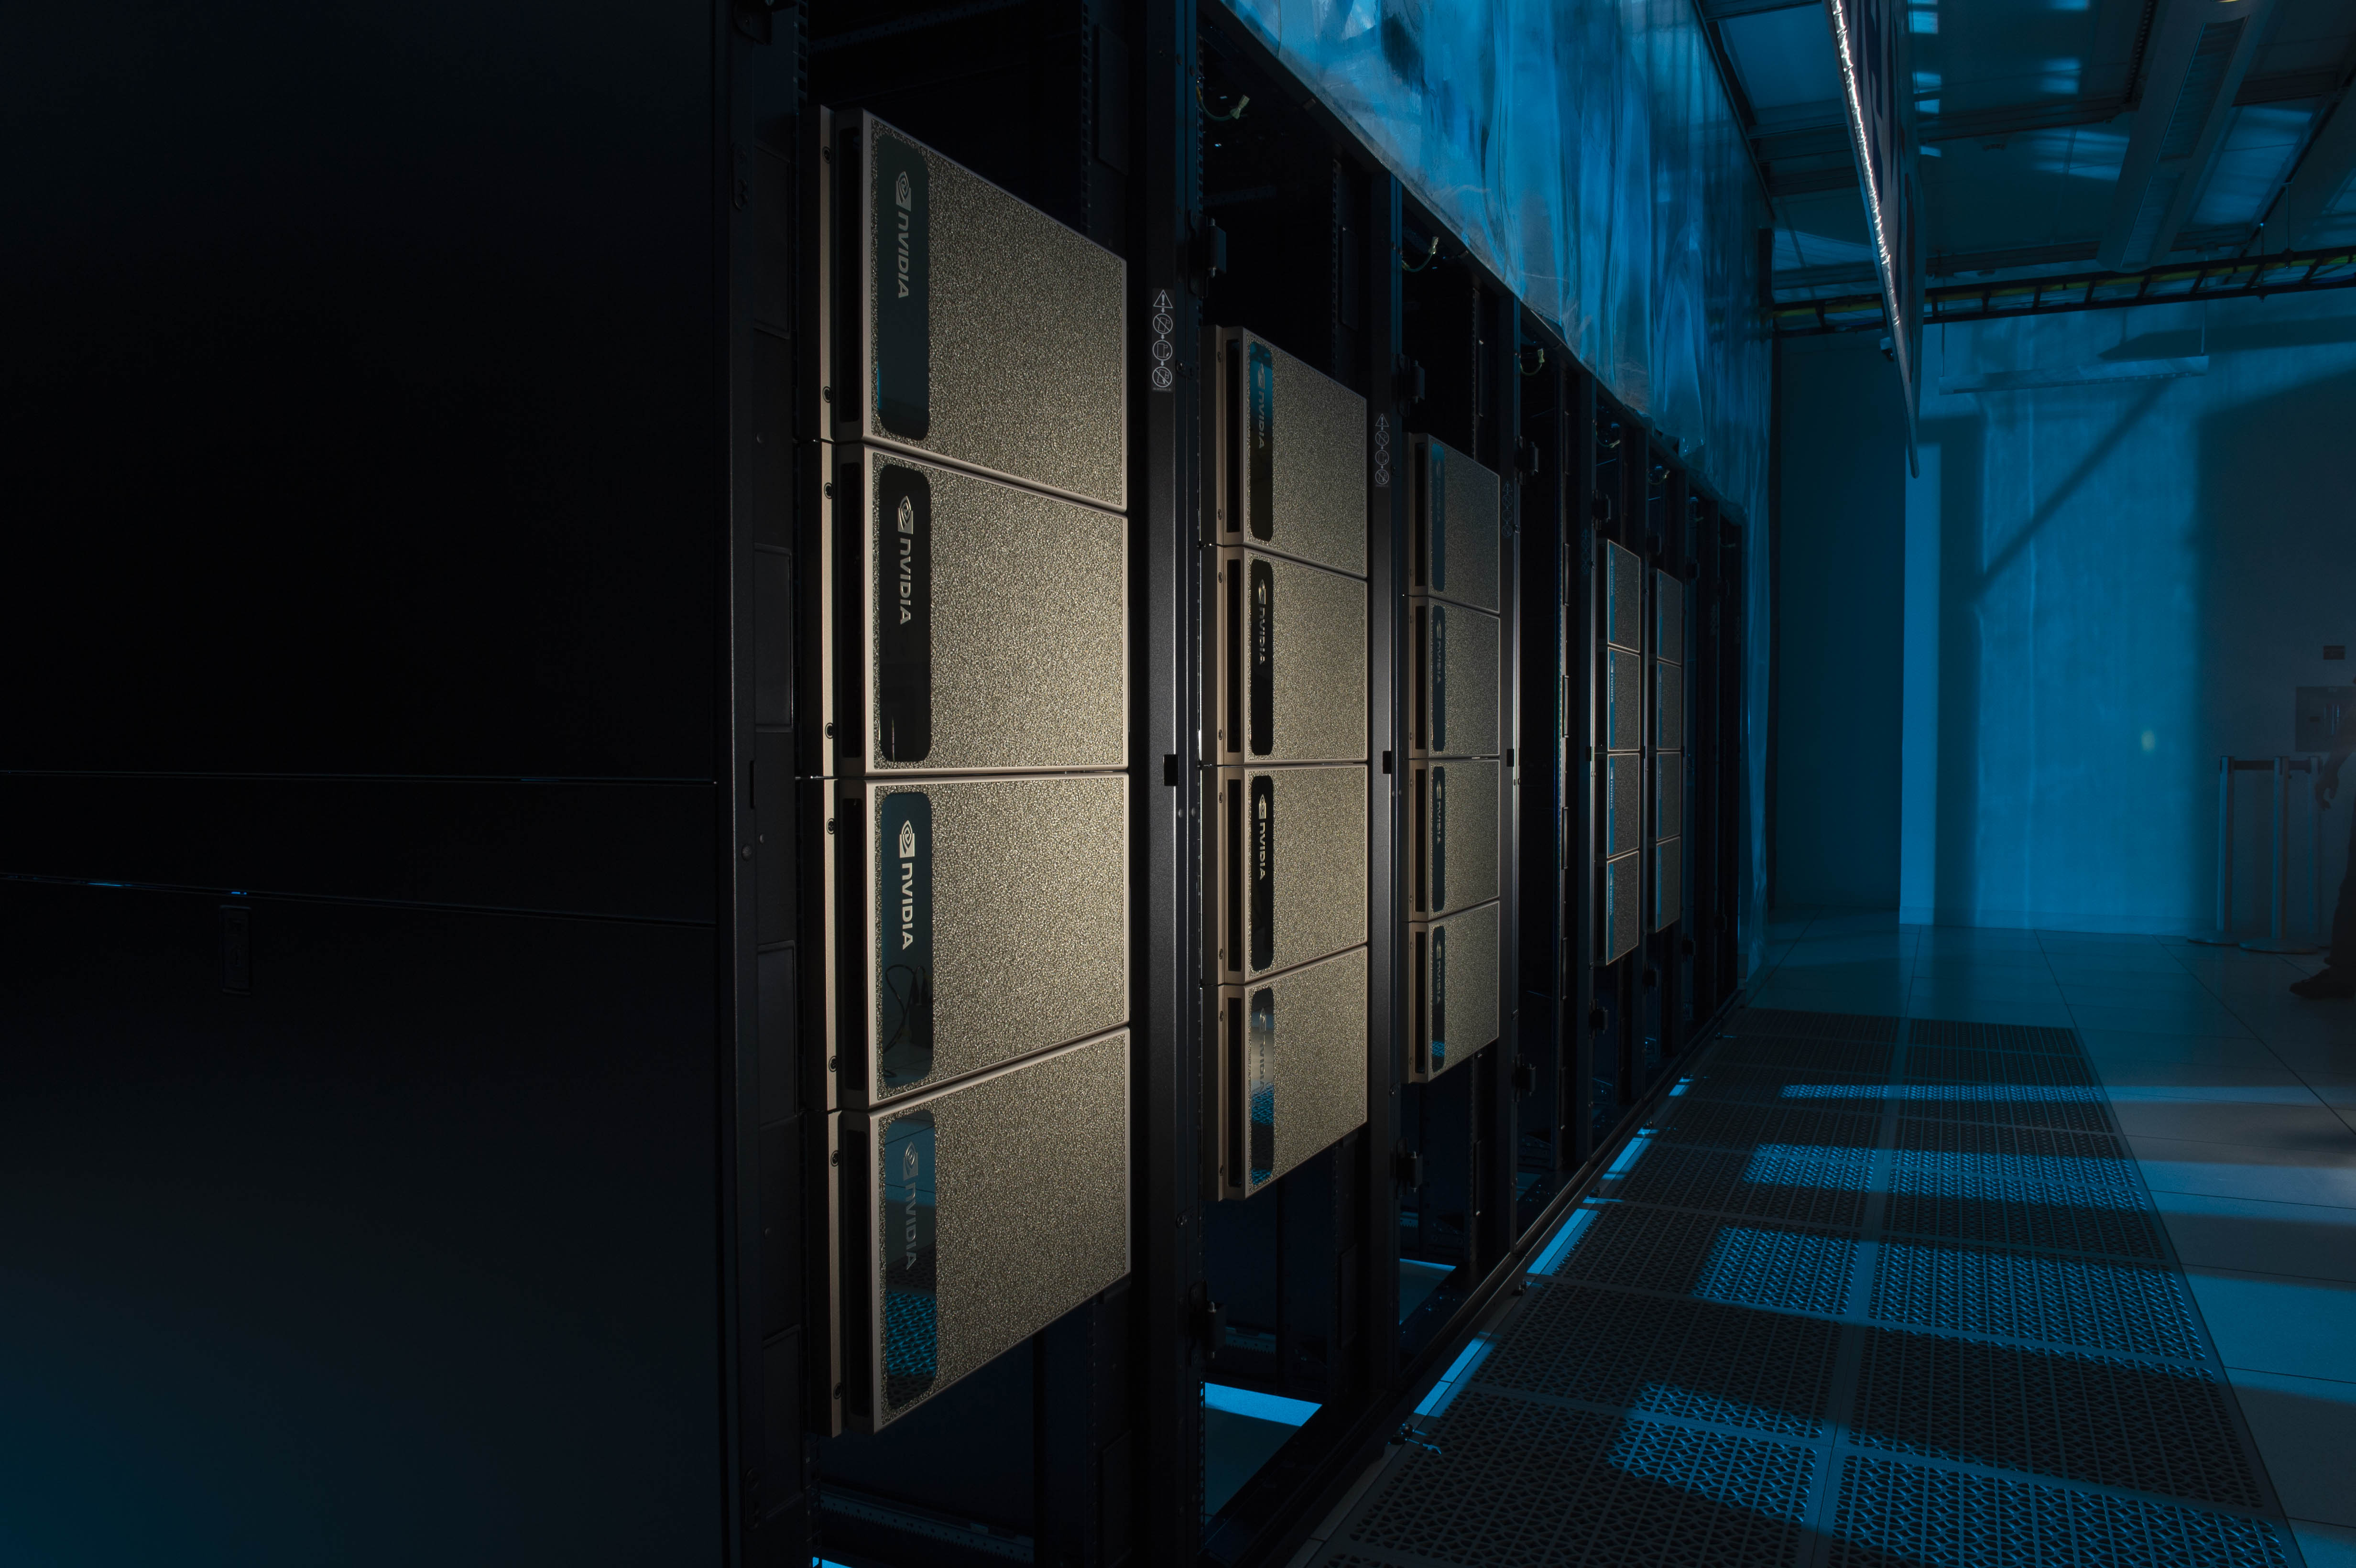
\includegraphics[width=\textwidth]{figures/superpod.jpg}
\end{center}
\end{column}
\end{columns}
\end{frame}

\begin{frame}{SMU HPC File Systems}
\begin{description}
\item[\$HOME]
\begin{itemize}
  \item Default file system when logging into a cluster.
  \item Space should be used to write, edit, compile programs, and job
        submission scripts, etc.
  \item Restricted by quotas (200 GB) and backed-up.
  \item Each cluster has it's own \mintinline{sh}{$HOME}.
\end{itemize}
\item[\$WORK]
\begin{itemize}
  \item Designed for longer term storage than \mintinline{sh}{$HOME}.
  \item Restricted by quotas (8 TB) and not backed-up.
  \item All clusters have access to \mintinline{sh}{$WORK}.
\end{itemize}
\item[\$SCRATCH]
\begin{itemize}
  \item High-performance scratch space.
  \item Treat \mintinline{sh}{$SCRATCH} as a volatile file system.
  \item Restricted by quotas to 60 days and not backed-up.
  \item Each cluster has it's own \mintinline{sh}{$SCRATCH}.
\end{itemize}
\end{description}
\end{frame}

%\begin{frame}{Unversity Data Center (UDC)}
%\begin{columns}
%\begin{column}{0.5\textwidth}
%\begin{center}
%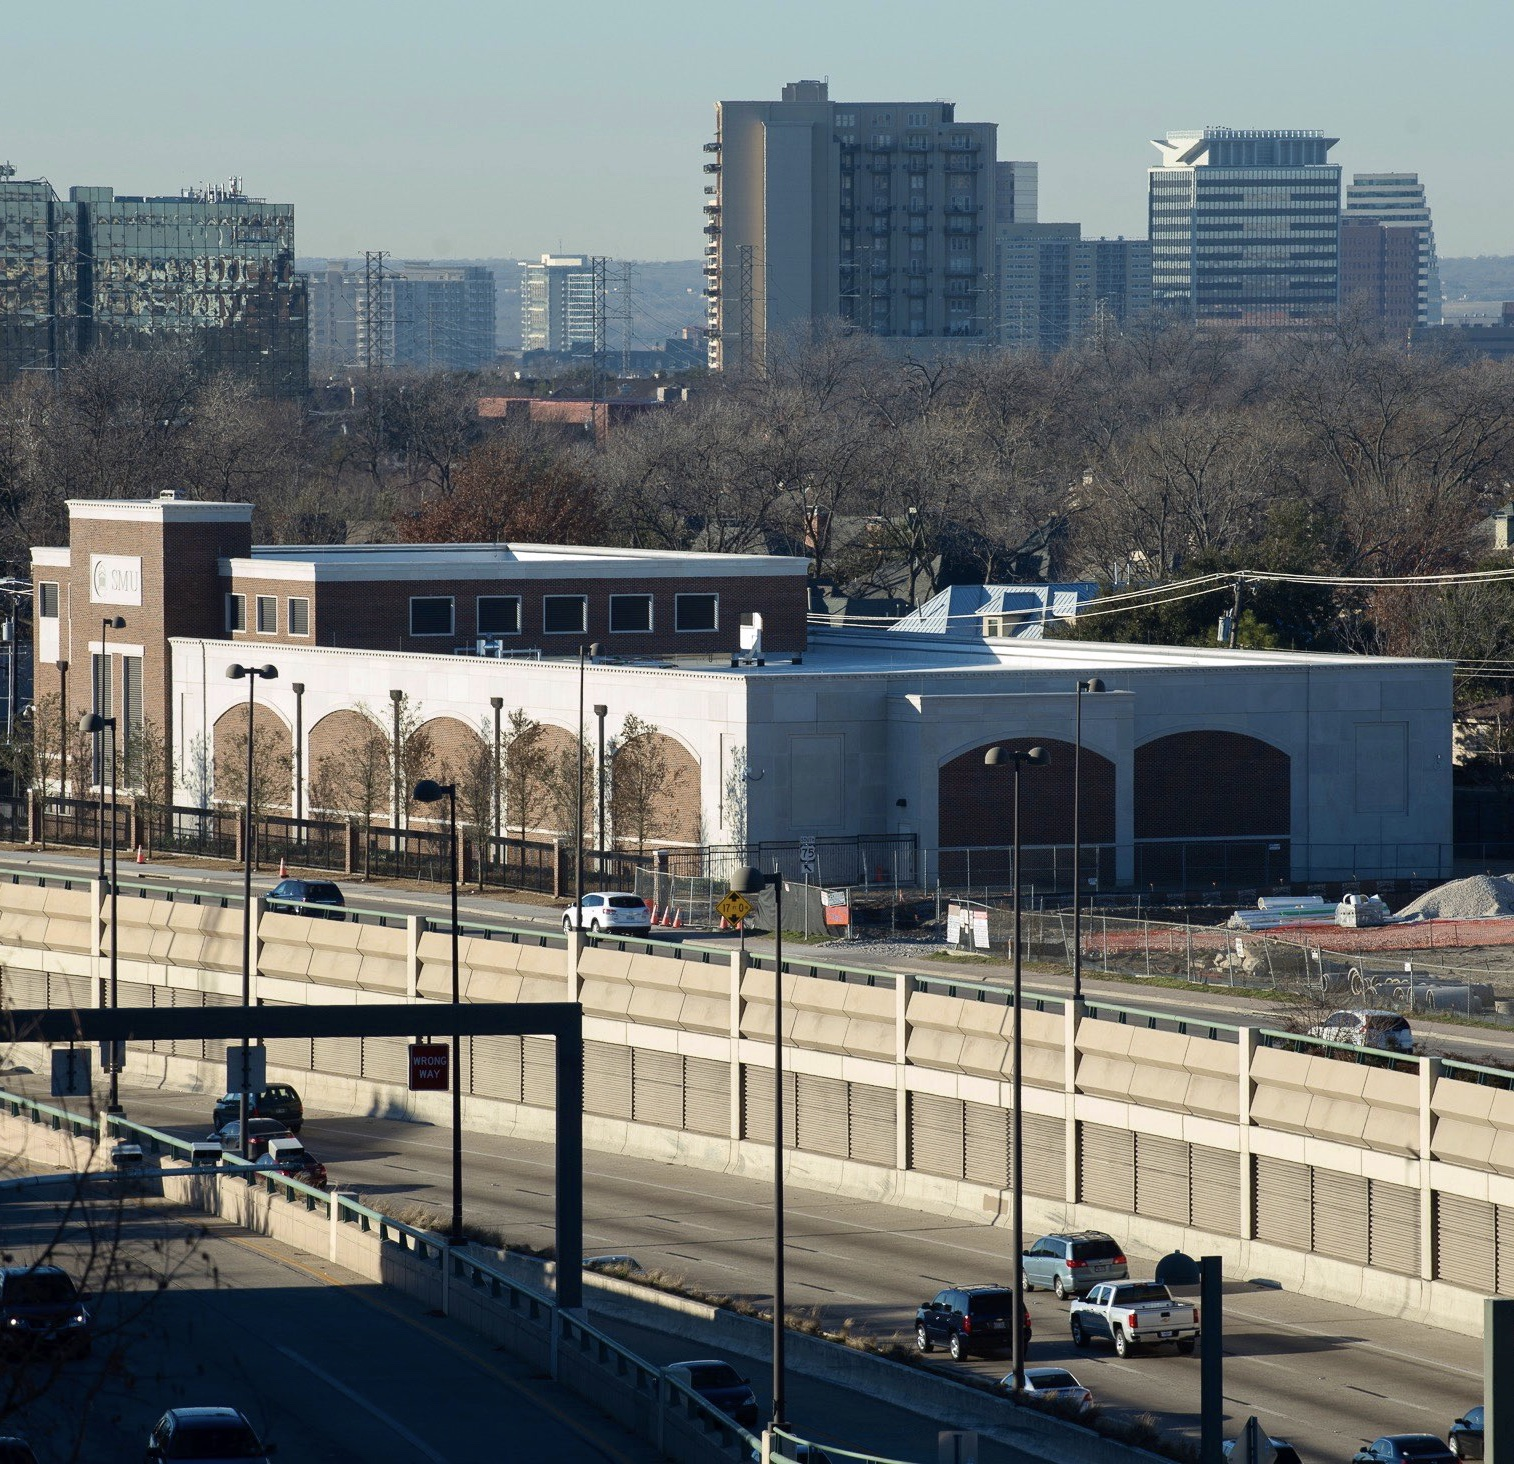
\includegraphics[width=\textwidth]{figures/udc_1.jpg}
%\end{center}
%\end{column}
%\begin{column}{0.5\textwidth}
%\begin{center}
%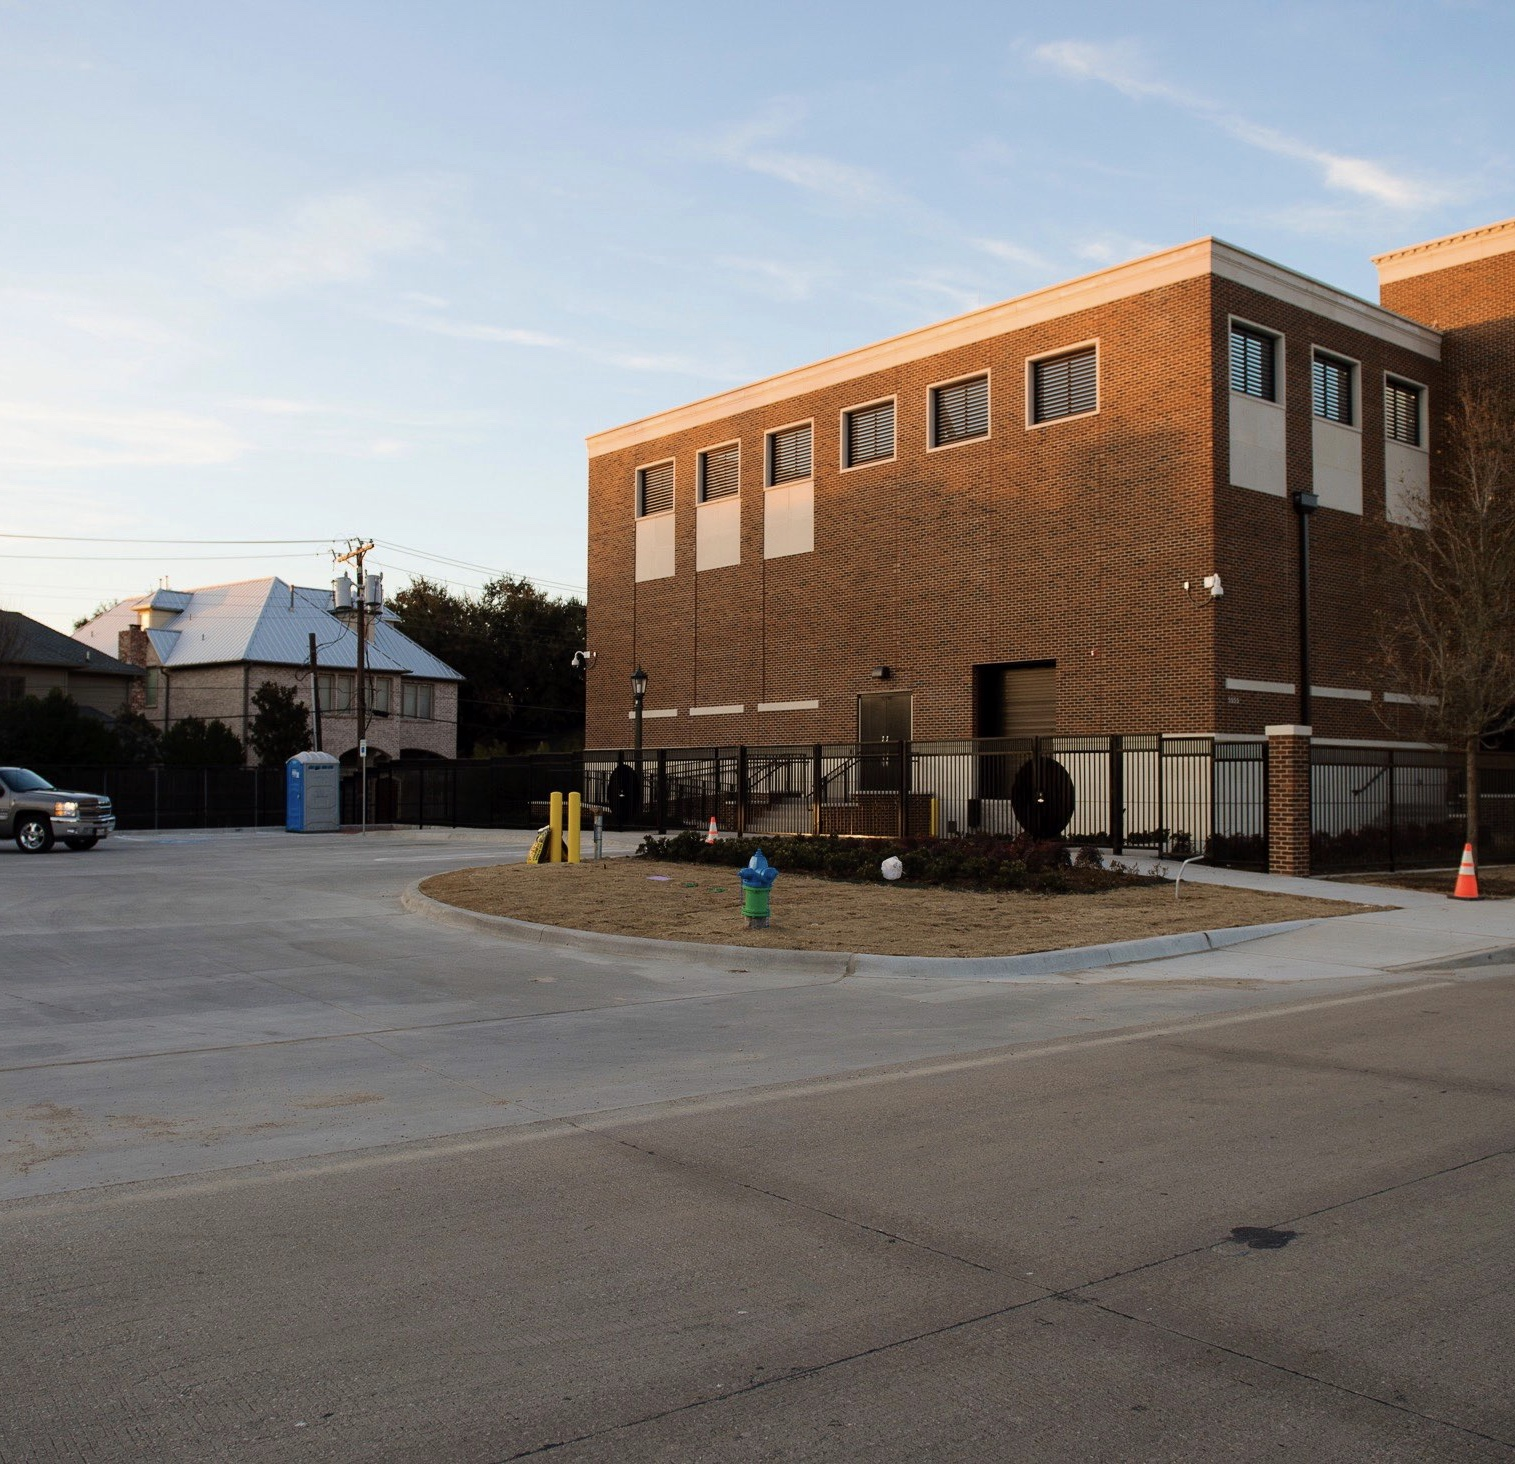
\includegraphics[width=\textwidth]{figures/udc_2.jpg}
%\end{center}
%\end{column}
%\end{columns}
%\end{frame}
%
%\begin{frame}{ManeFrame II (M2)}
%\begin{columns}
%\begin{column}{0.5\textwidth}
%\begin{center}
%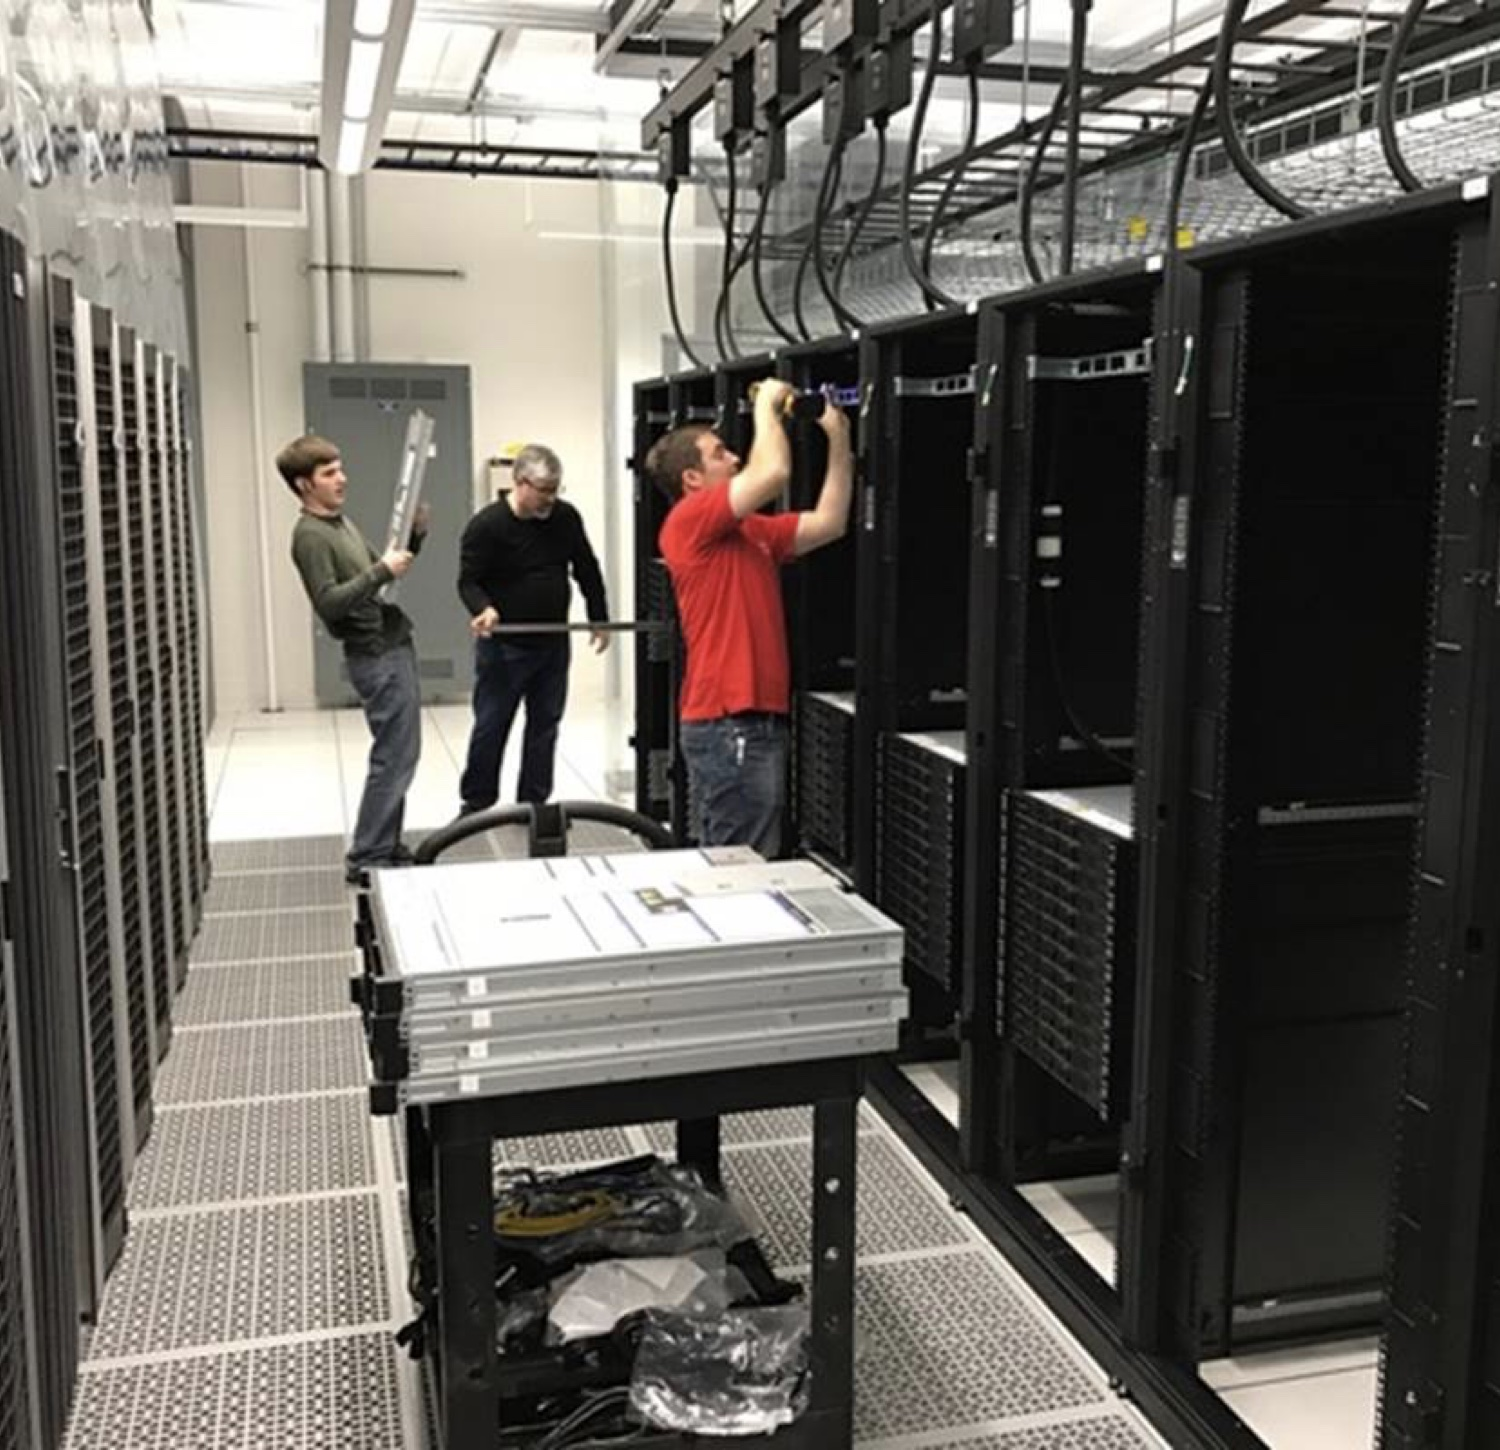
\includegraphics[width=\textwidth]{figures/m2_1.jpg}
%\end{center}
%\end{column}
%\begin{column}{0.5\textwidth}
%\begin{center}
%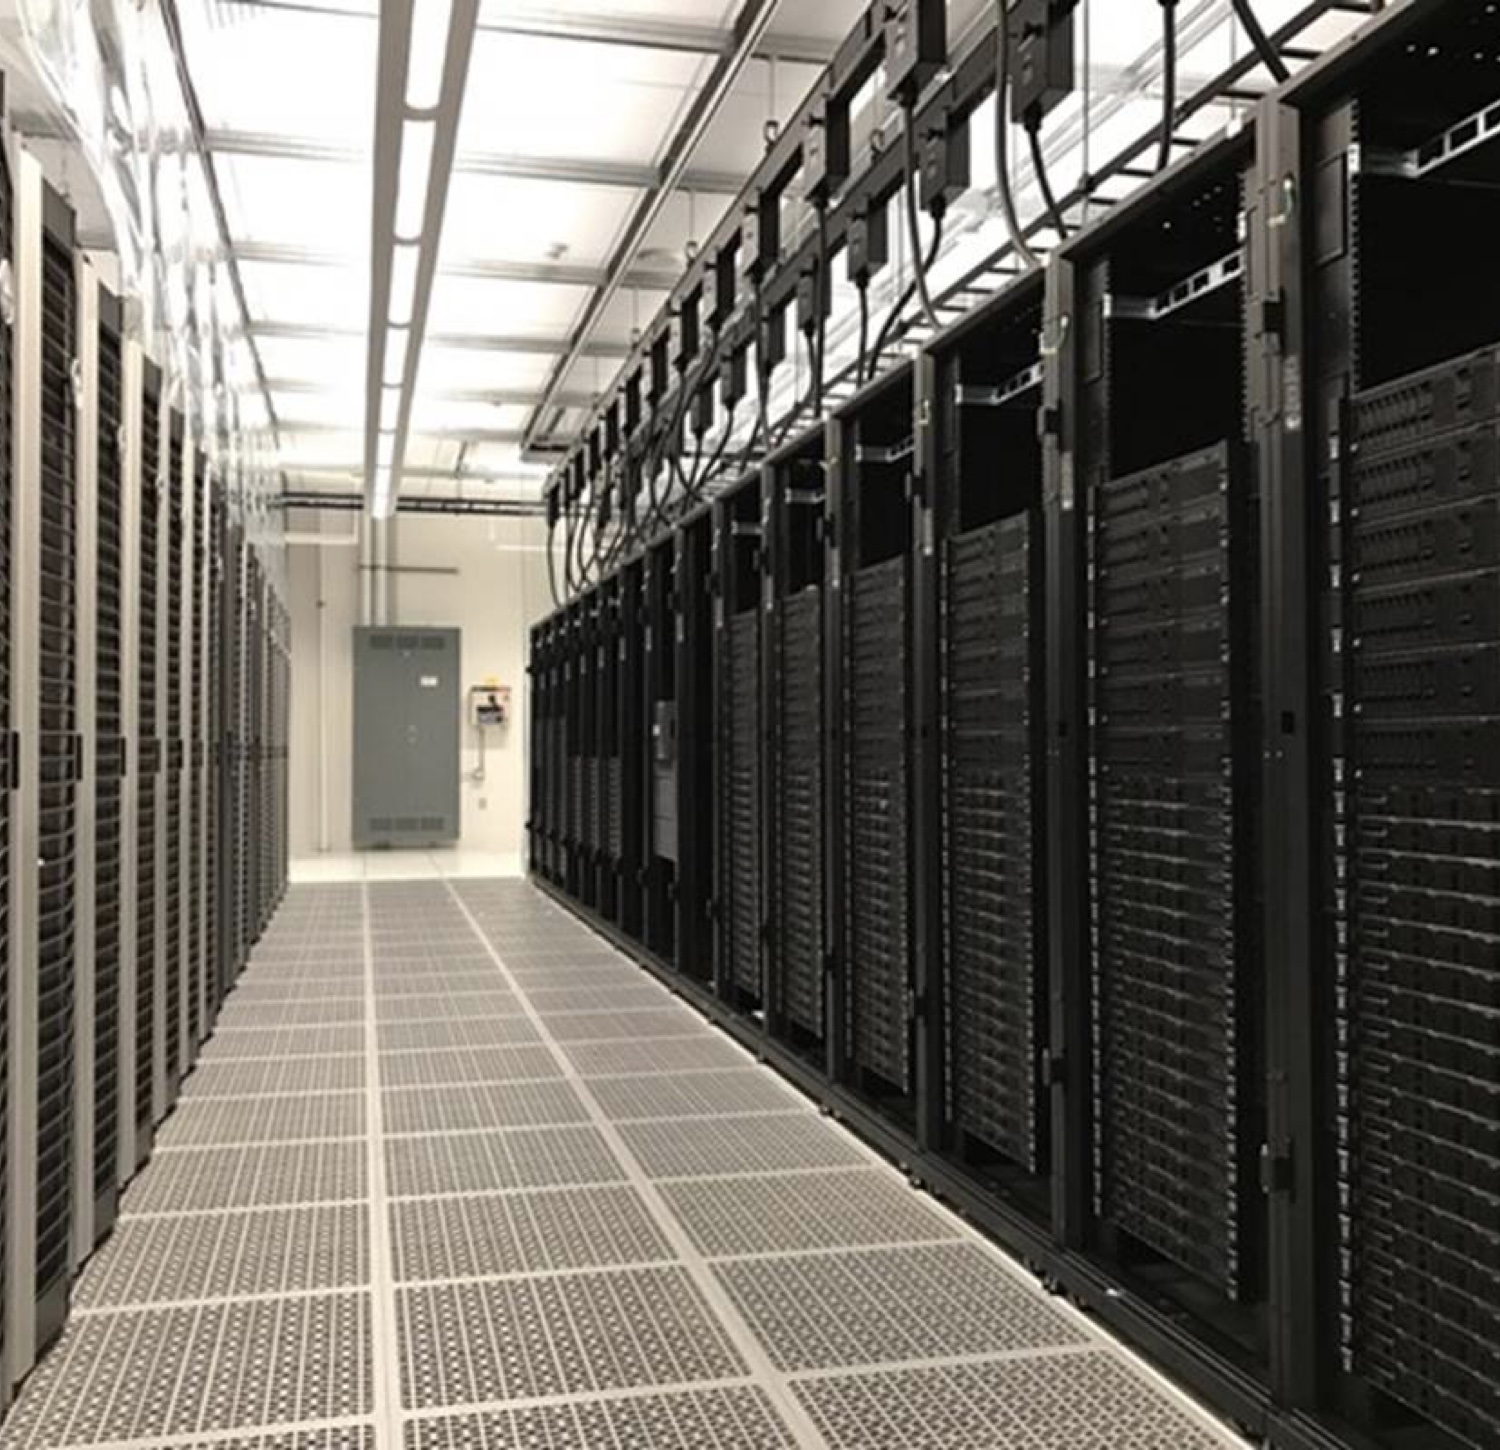
\includegraphics[width=\textwidth]{figures/m2_2.jpg}
%\end{center}
%\end{column}
%\end{columns}
%\end{frame}
%
%\begin{frame}{Hot Aisle Containment}
%\begin{columns}
%\begin{column}{0.5\textwidth}
%\begin{center}
%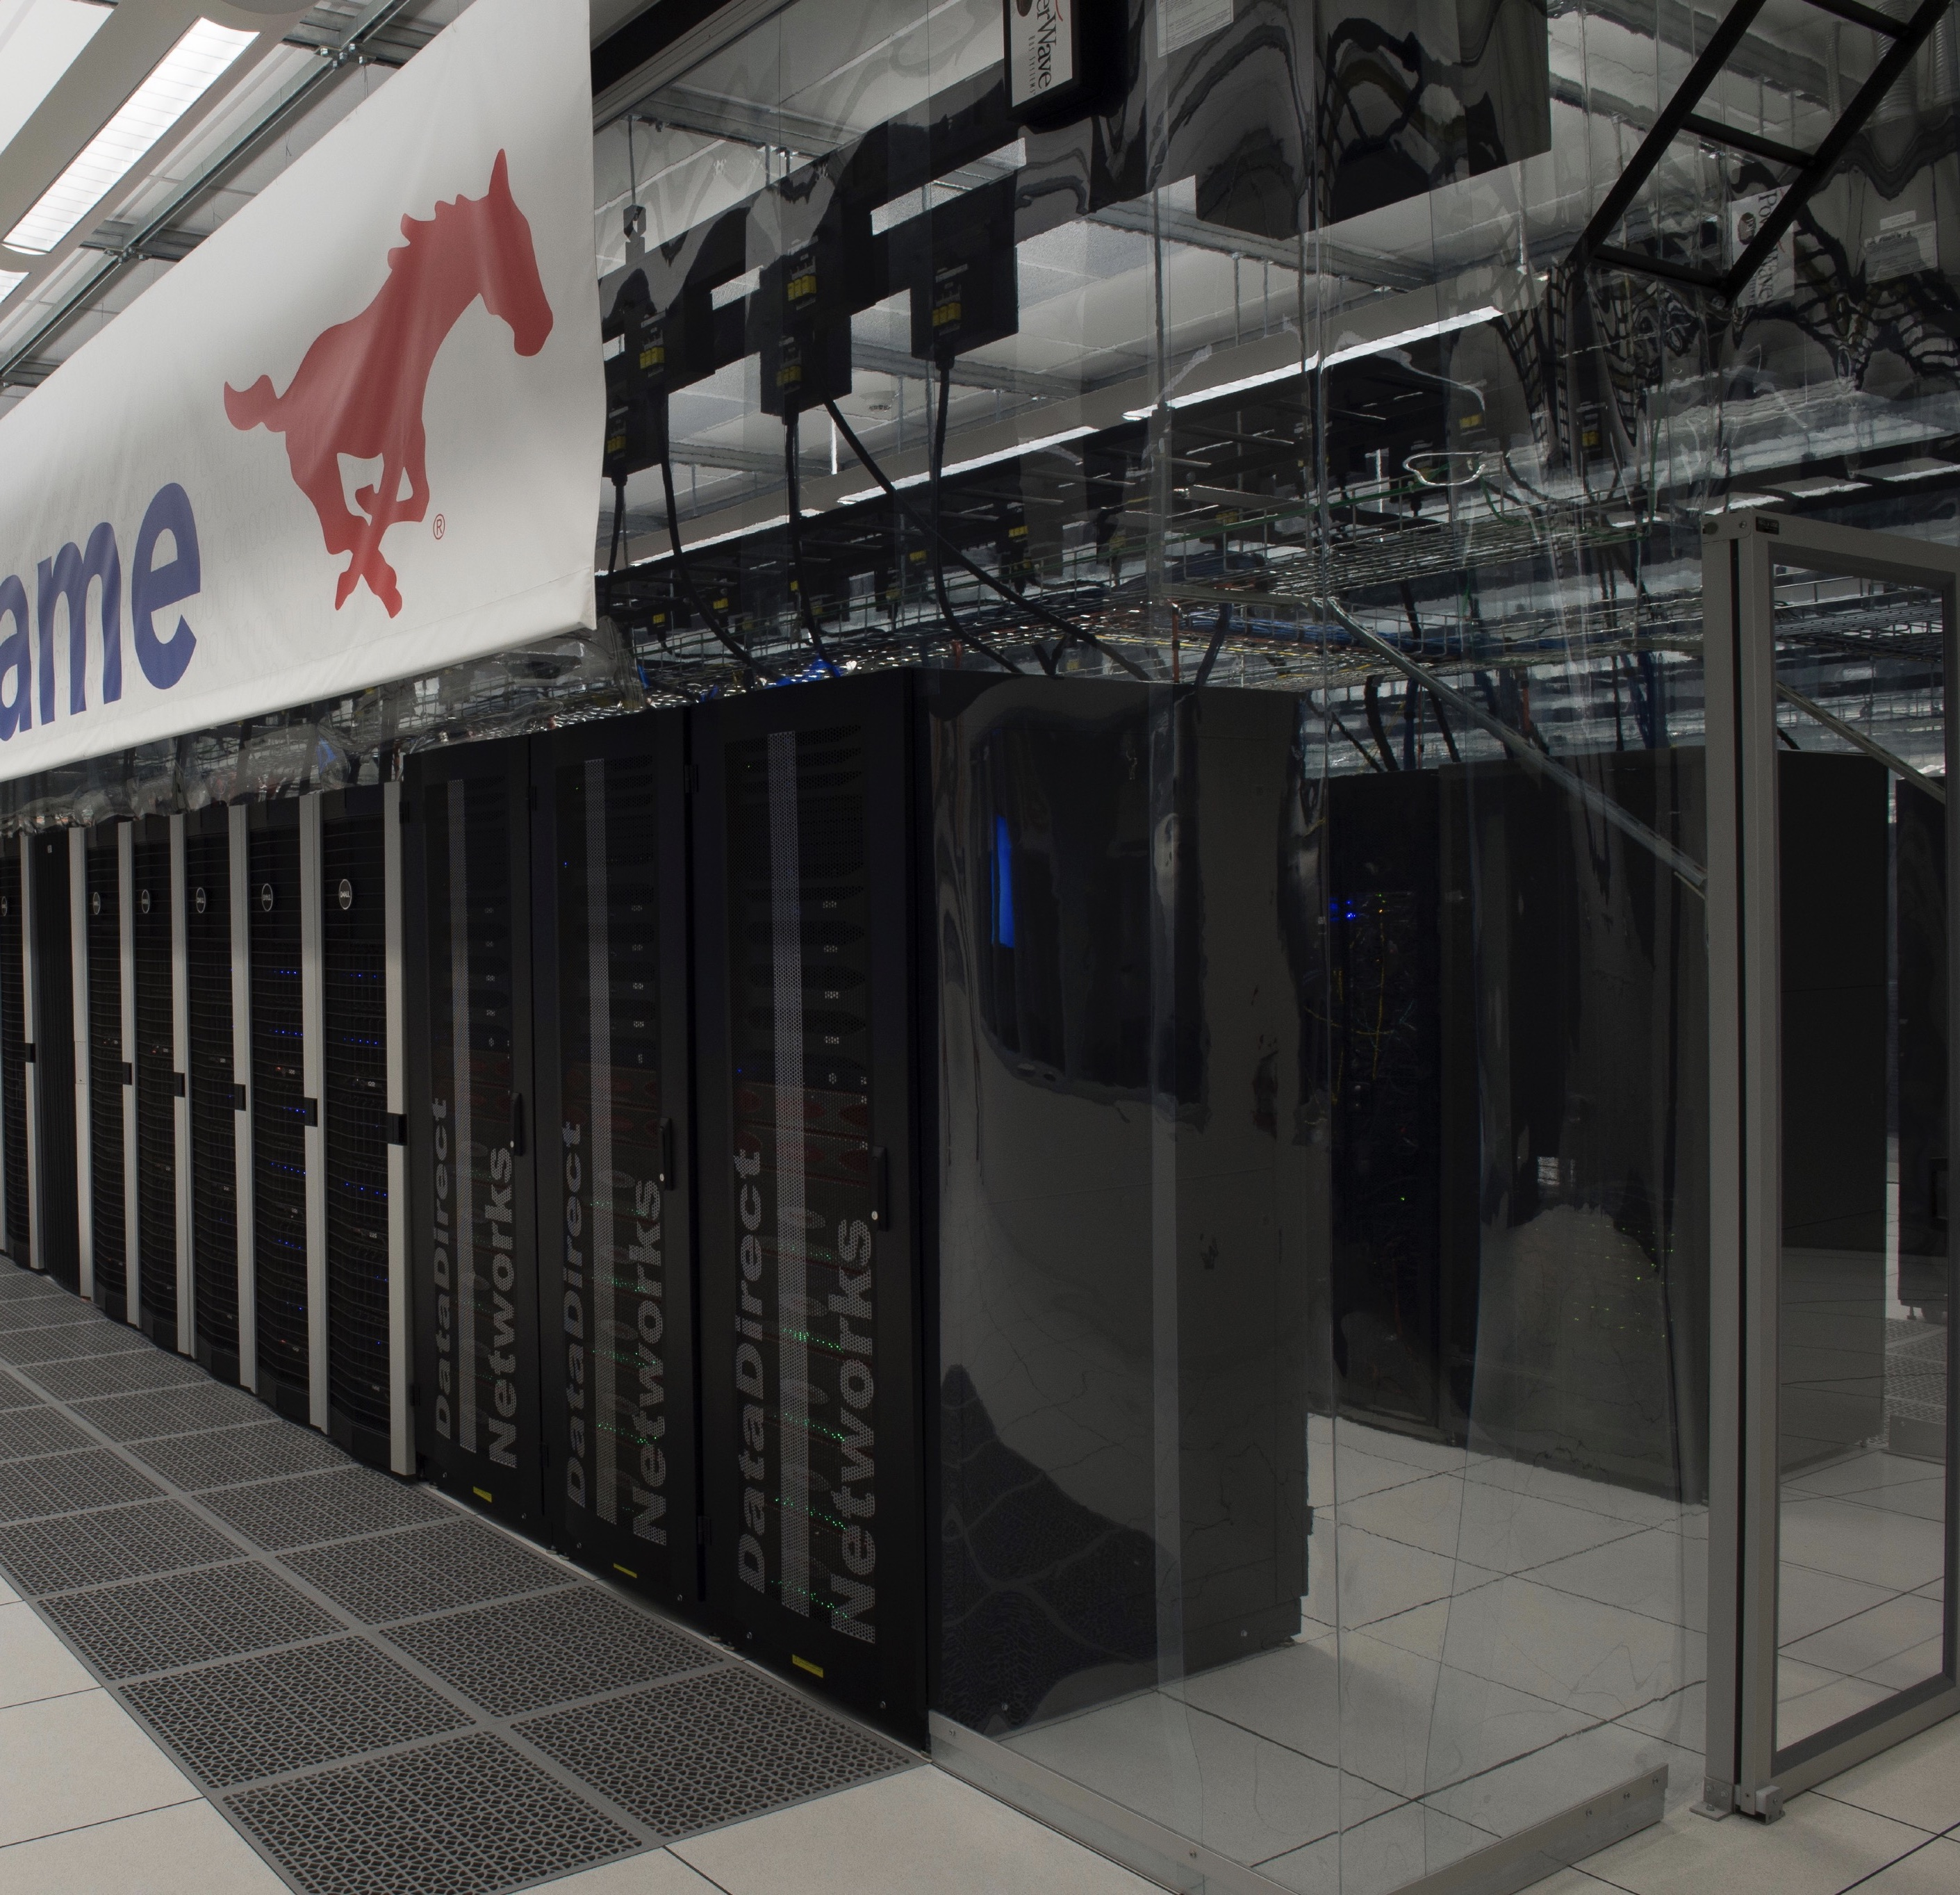
\includegraphics[width=\textwidth]{figures/hot_aisle_1.jpg}
%\end{center}
%\end{column}
%\begin{column}{0.5\textwidth}
%\begin{center}
%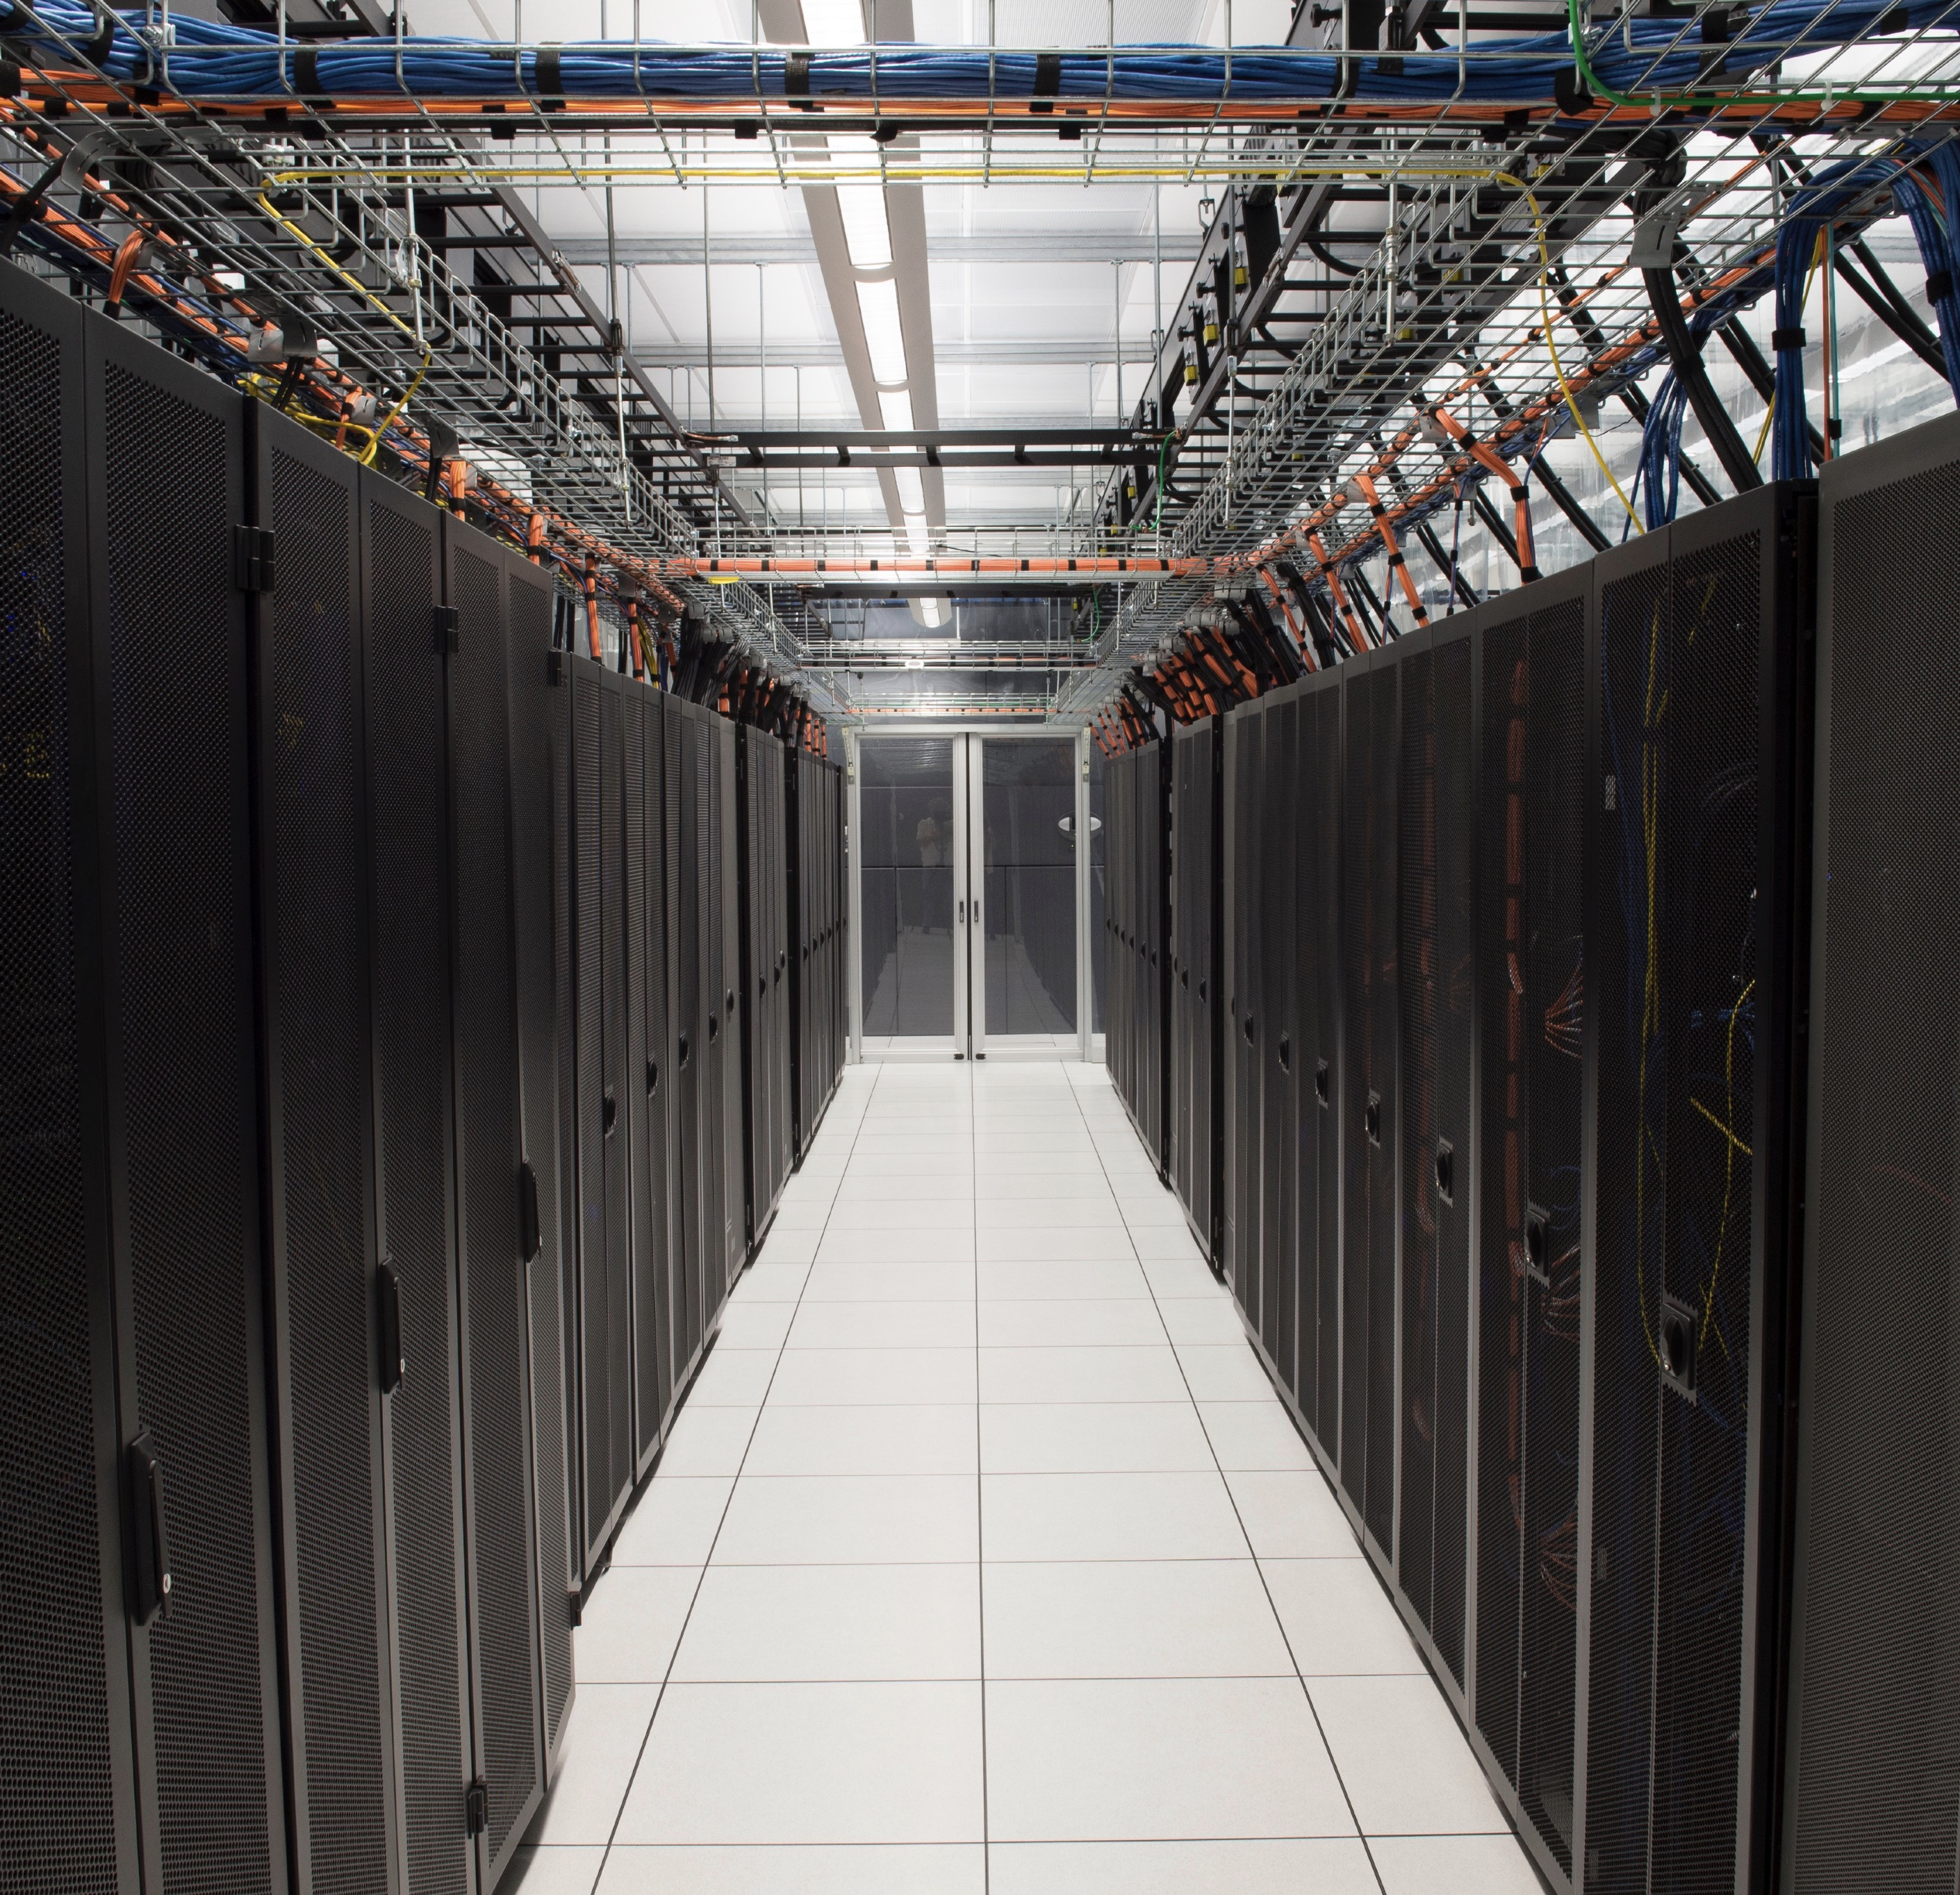
\includegraphics[width=\textwidth]{figures/hot_aisle_2.jpg}
%\end{center}
%\end{column}
%\end{columns}
%\end{frame}
%
%\begin{frame}{Cooling and Power}
%\begin{columns}
%\begin{column}{0.5\textwidth}
%\begin{center}
%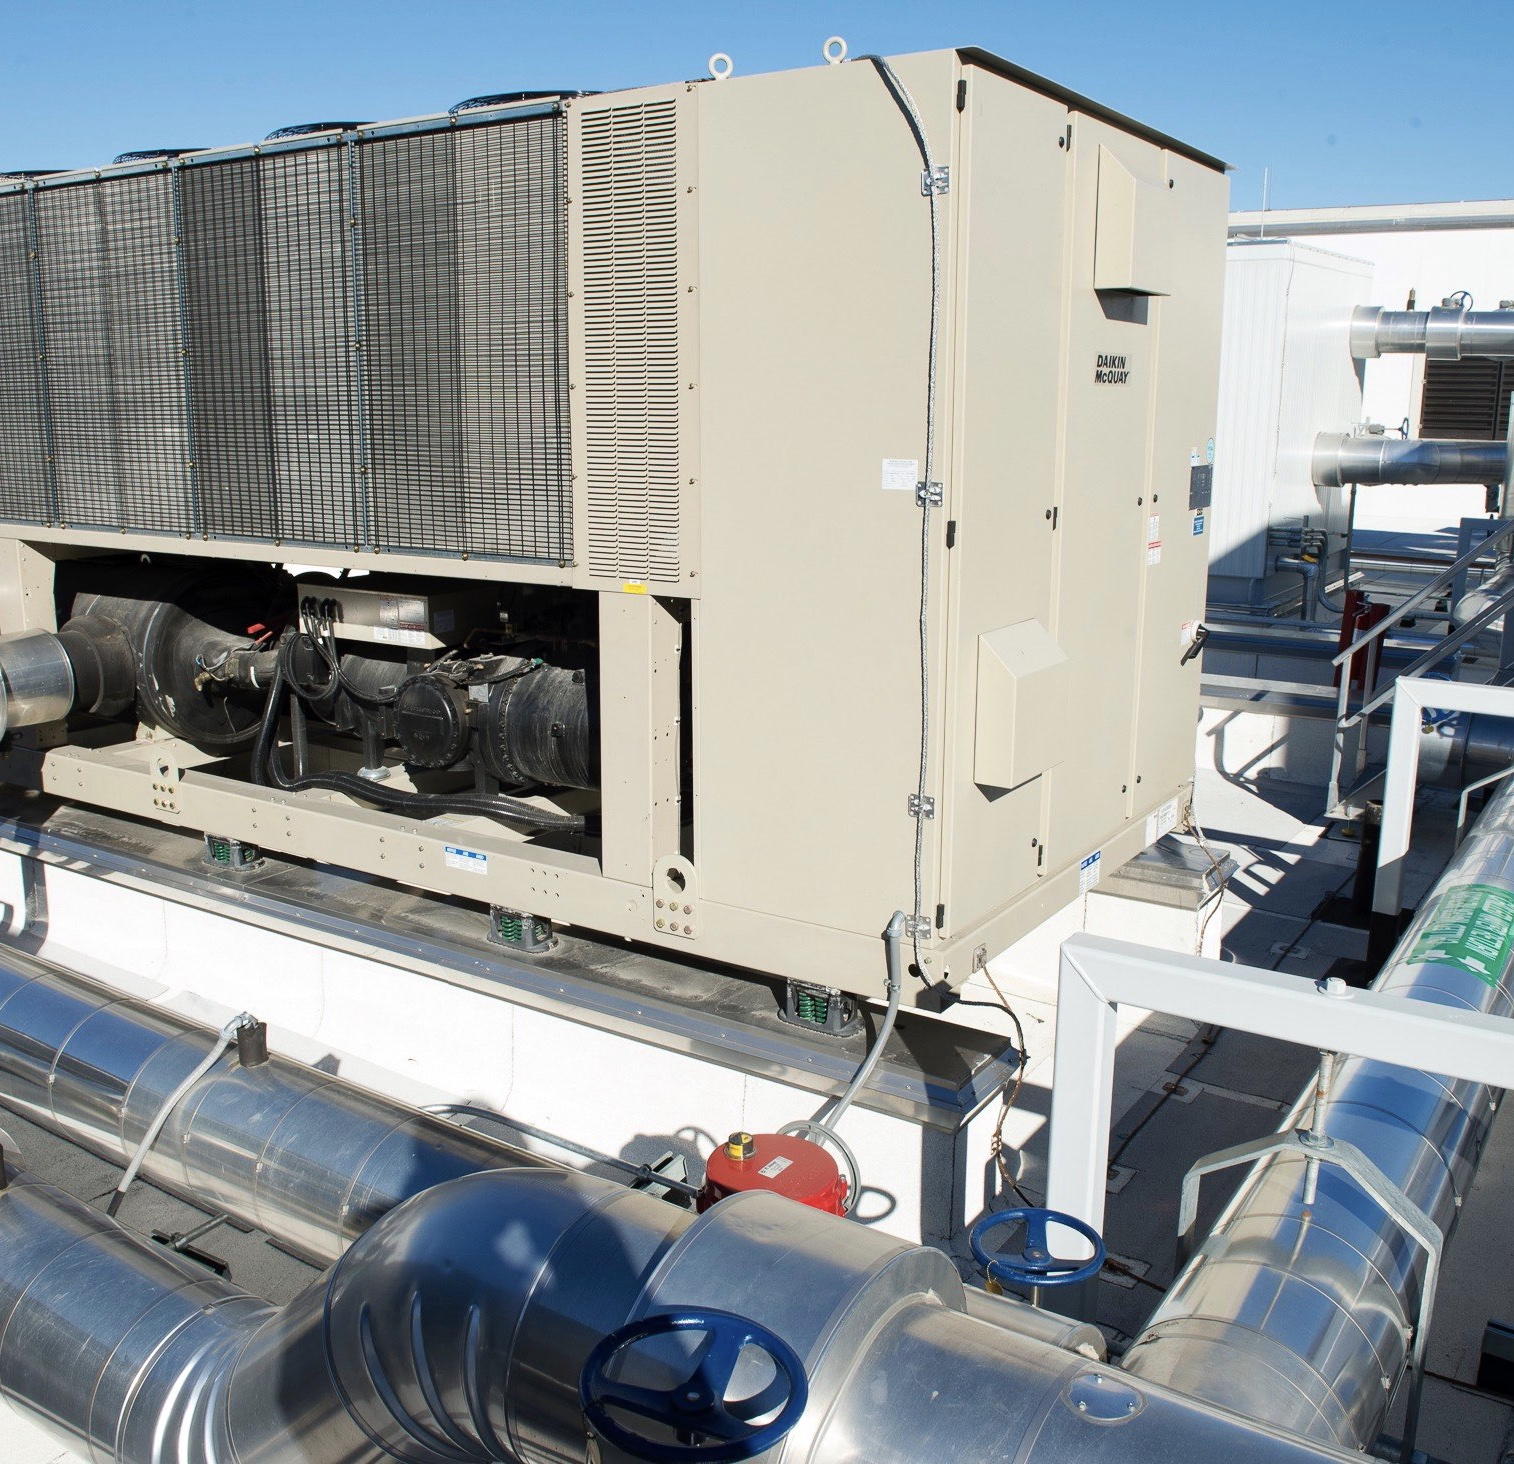
\includegraphics[width=\textwidth]{figures/cooling.jpg}
%\end{center}
%\end{column}
%\begin{column}{0.5\textwidth}
%\begin{center}
%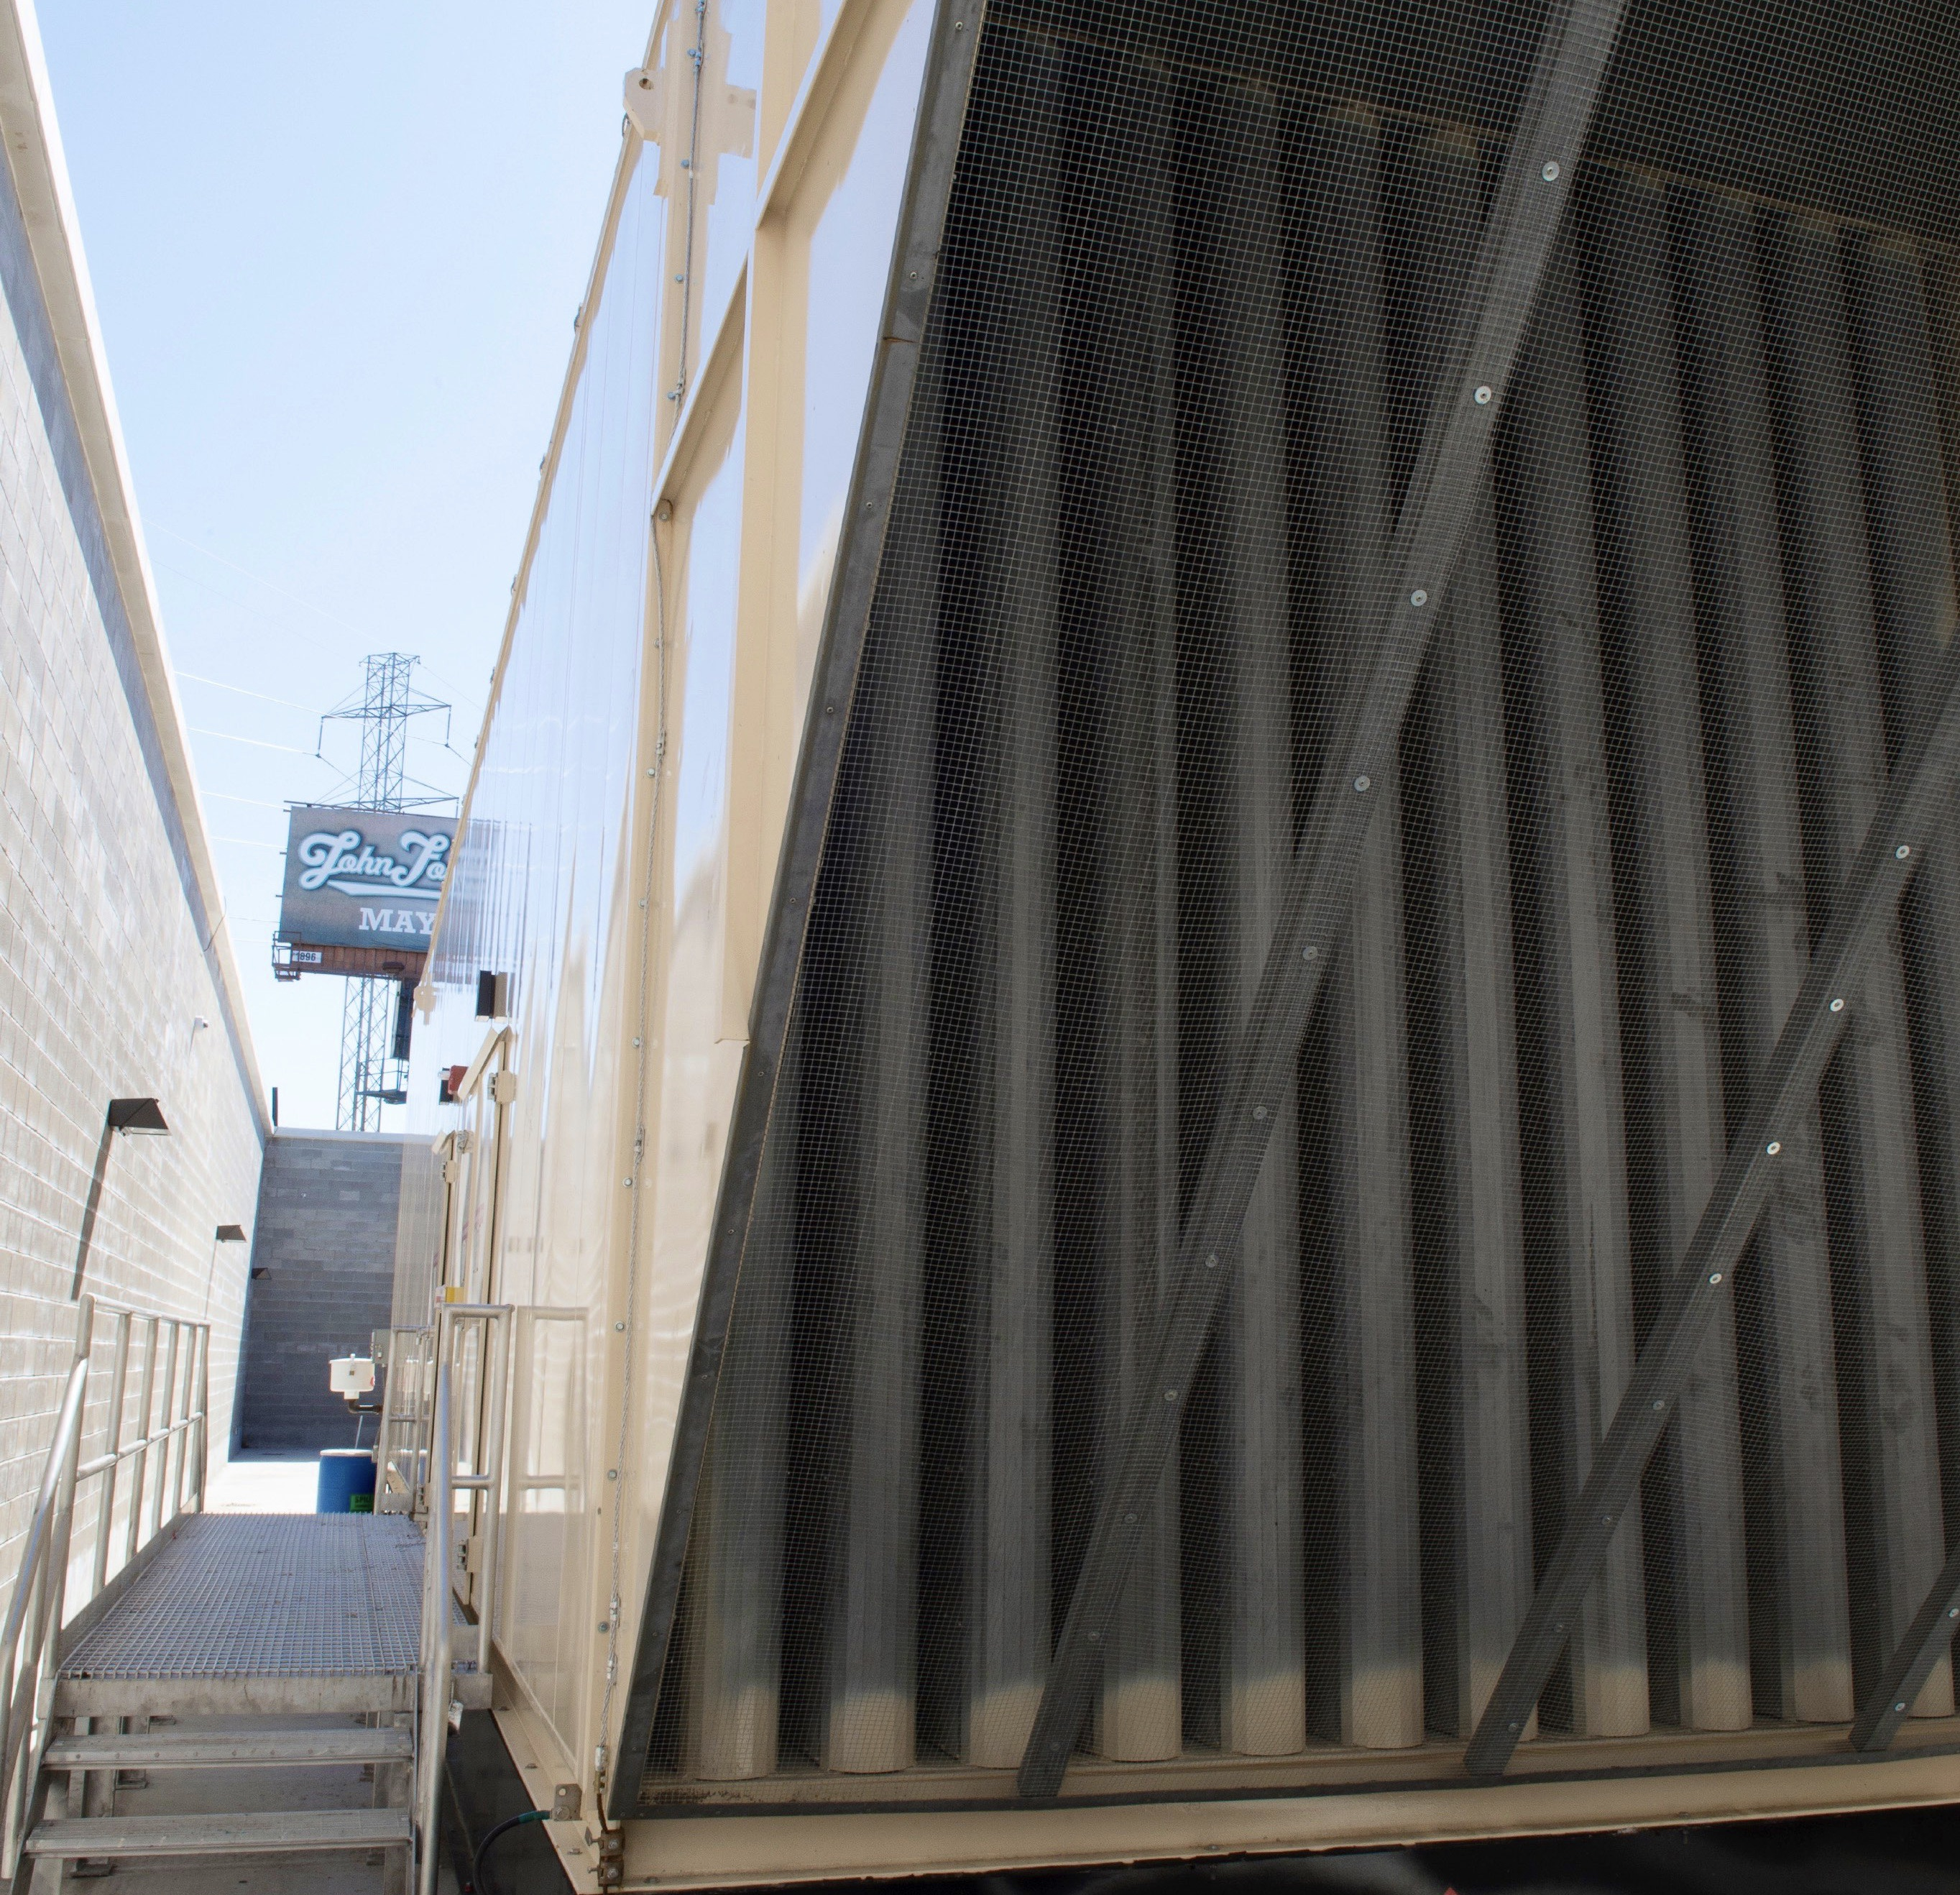
\includegraphics[width=\textwidth]{figures/power.jpg}
%\end{center}
%\end{column}
%\end{columns}
%\end{frame}


%\section{Compute Hardware}

\begin{frame}{Parallel Computations}
\begin{center}
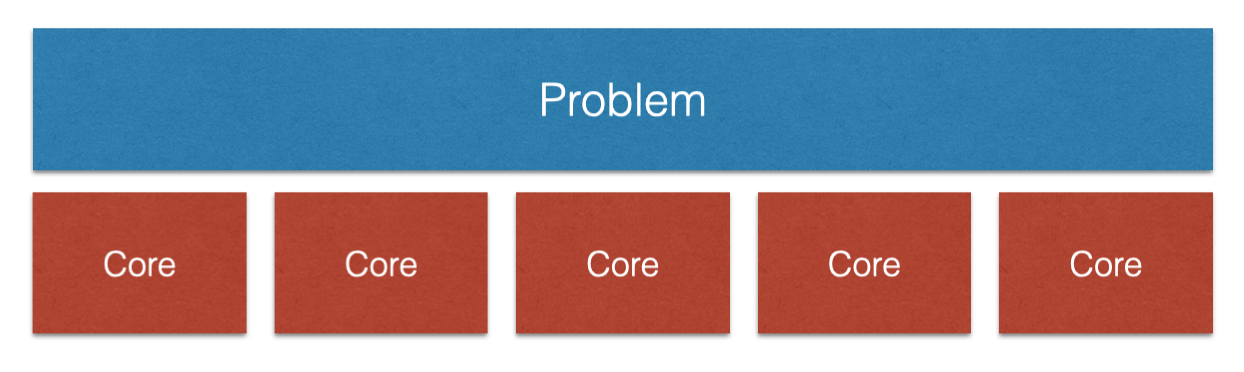
\includegraphics[width=0.65\linewidth]{figures/problem_over_cores.png}
\end{center}
\begin{itemize}
\item Using multiple processing units (cores, etc.) simultaneously to perform a computation
\item Use multiple computers to store data for large problems
\item Essentially all modern CPUs have multiple cores
\end{itemize}
\end{frame}

\begin{frame}{Parallel Hardware}
\begin{itemize}
\item Levels of parallelism
\item Vectorization
\item Multicore
\item Multi-CPU
\item Multi-Node
\item Threads versus processes
\end{itemize}
\end{frame}

\begin{frame}{Intel Xeon Phi Nodes}
\begin{columns}
\begin{column}{0.5\textwidth}
\begin{itemize}
\item Intel Xeon Phi 7230 (also known as ``Knights Landing'' or ``KNL'') processors
\item 64 1.30 GHz cores based on the Atom ``Silvermont'' architecture
\item Cache: 32 MB L2
\item Cache: 16 GB of high bandwidth (400 GB/s) stacked memory
\item Memory: DDR4 2400 MHz, 115.2 GB/s
\item Vector Extensions: AVX-512 (512 bit width)
\item Hardware-based support for up to four concurrent threads
\end{itemize}
\end{column}
\begin{column}{0.5\textwidth}
\begin{center}
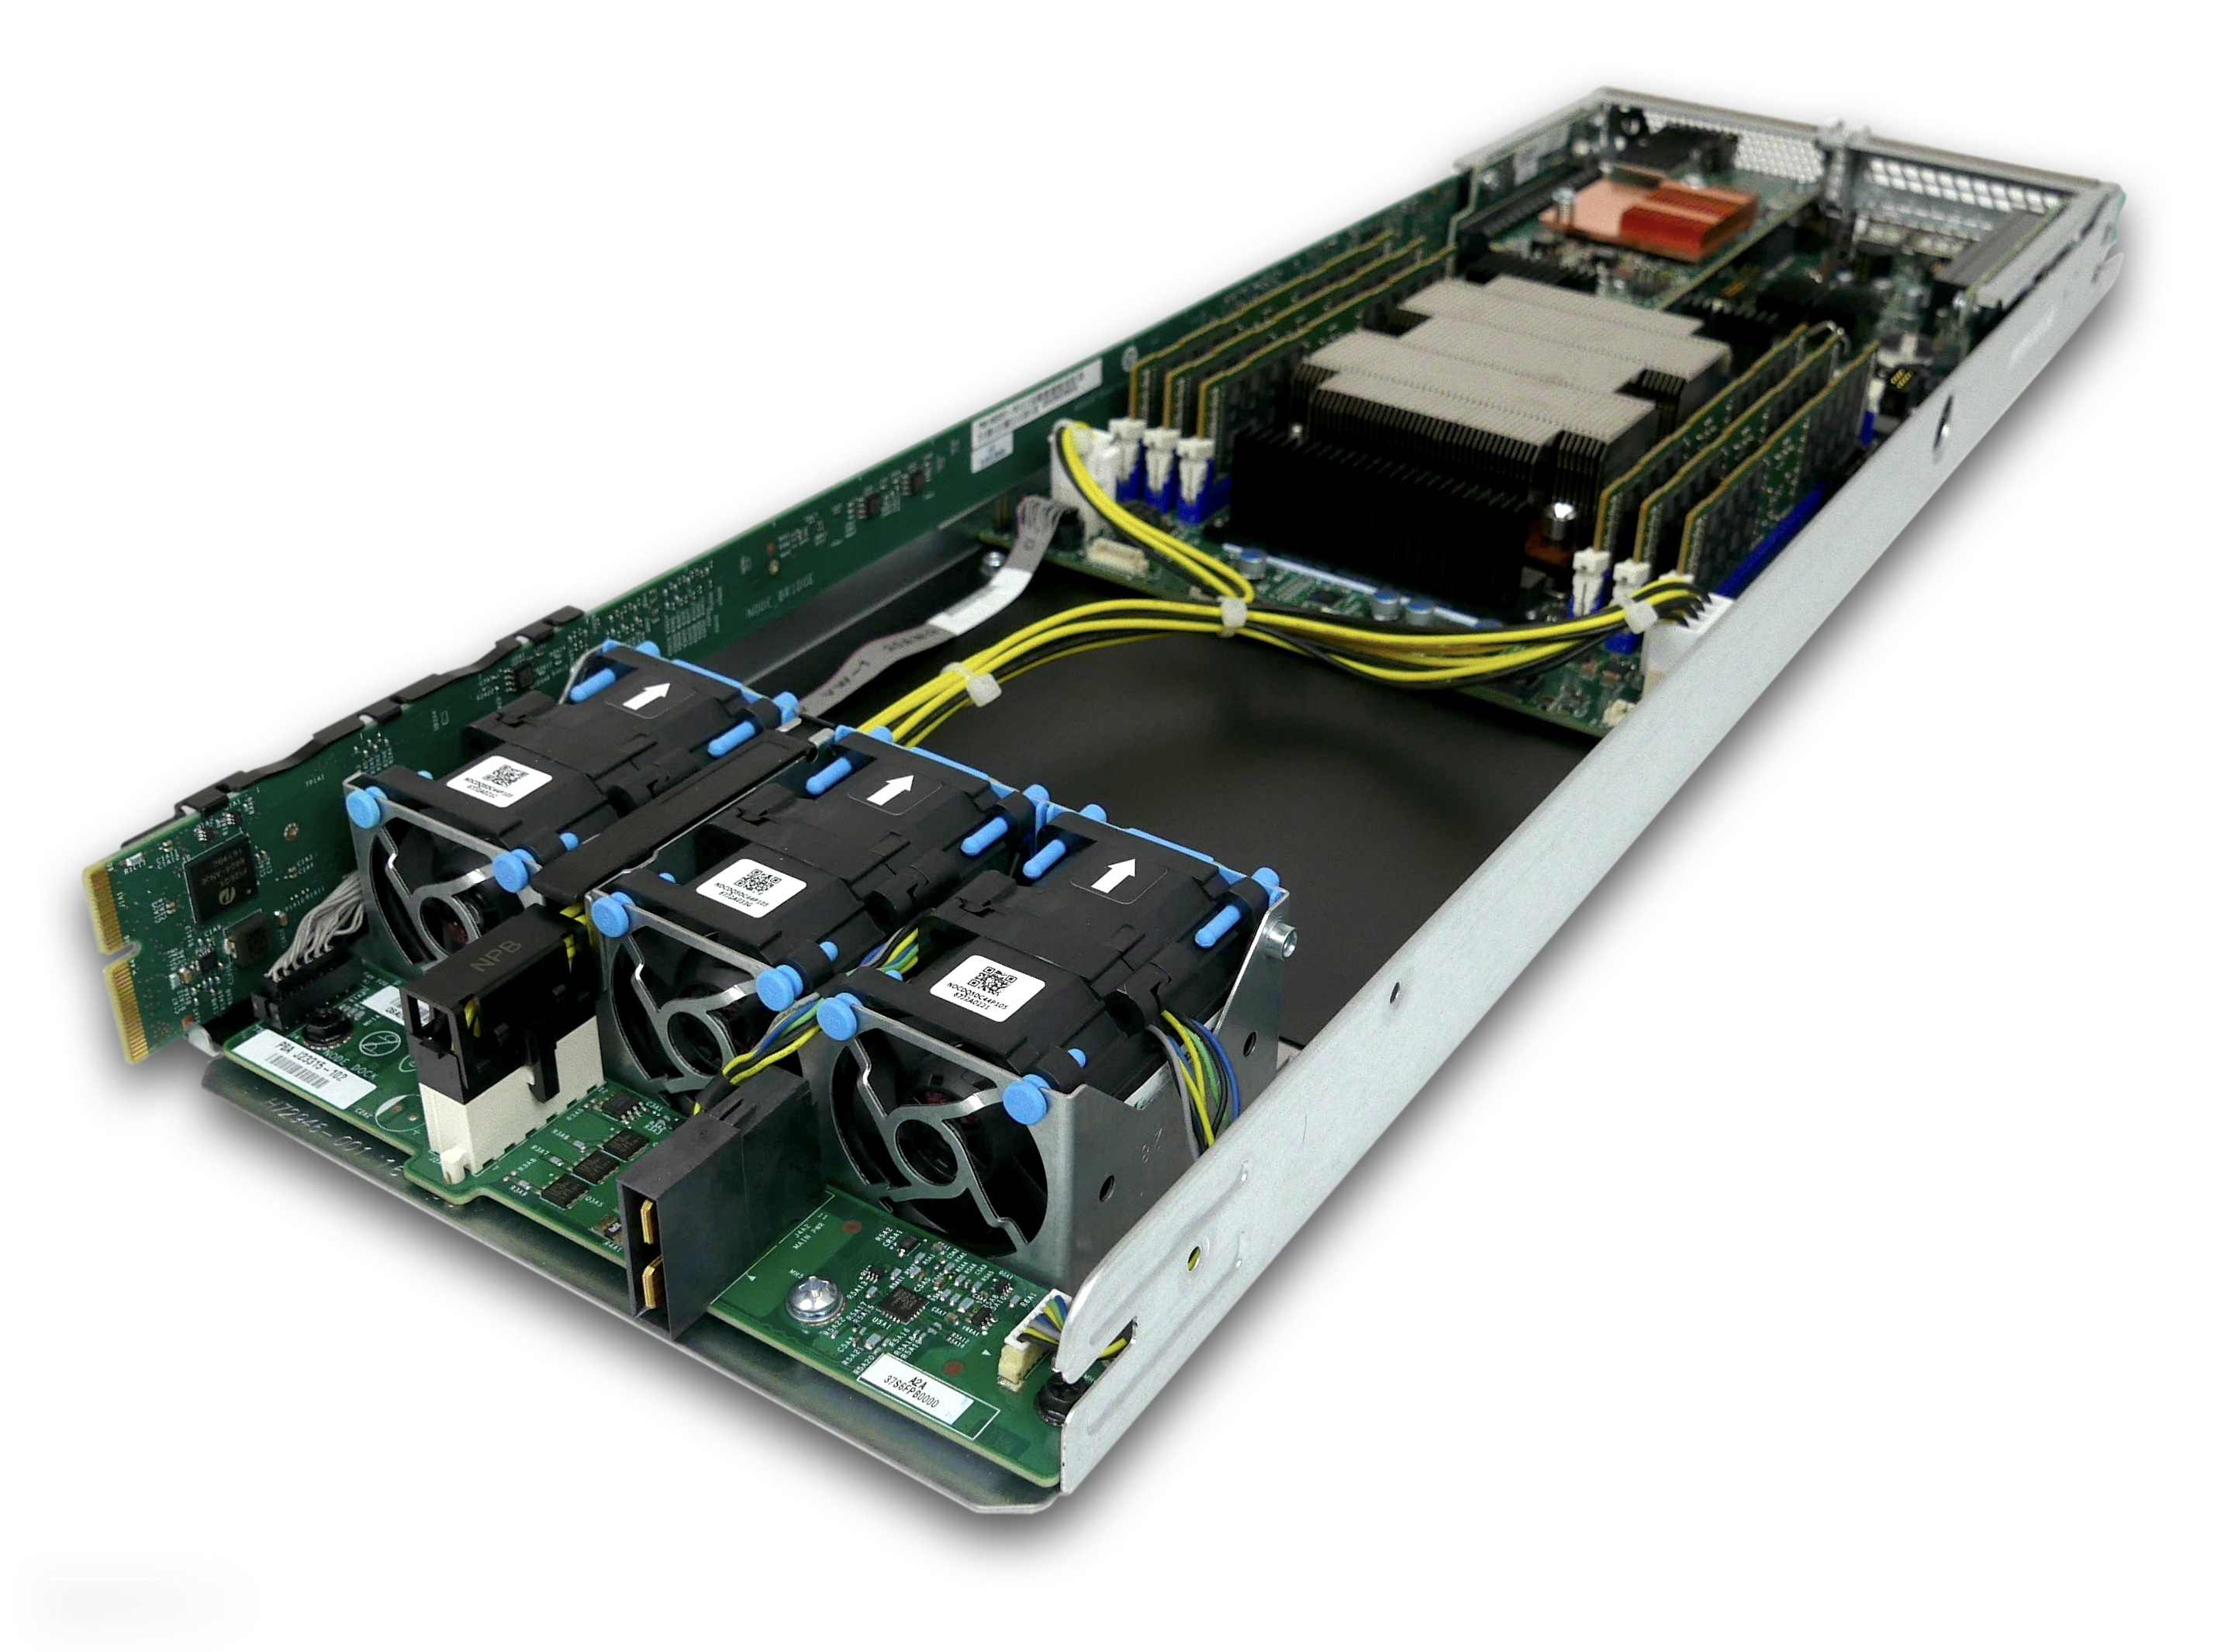
\includegraphics[width=\textwidth]{figures/mic_sled.jpg}
\end{center}
\end{column}
\end{columns}
\end{frame}

\begin{frame}{Intel Xeon Phi Nodes}
\begin{center}
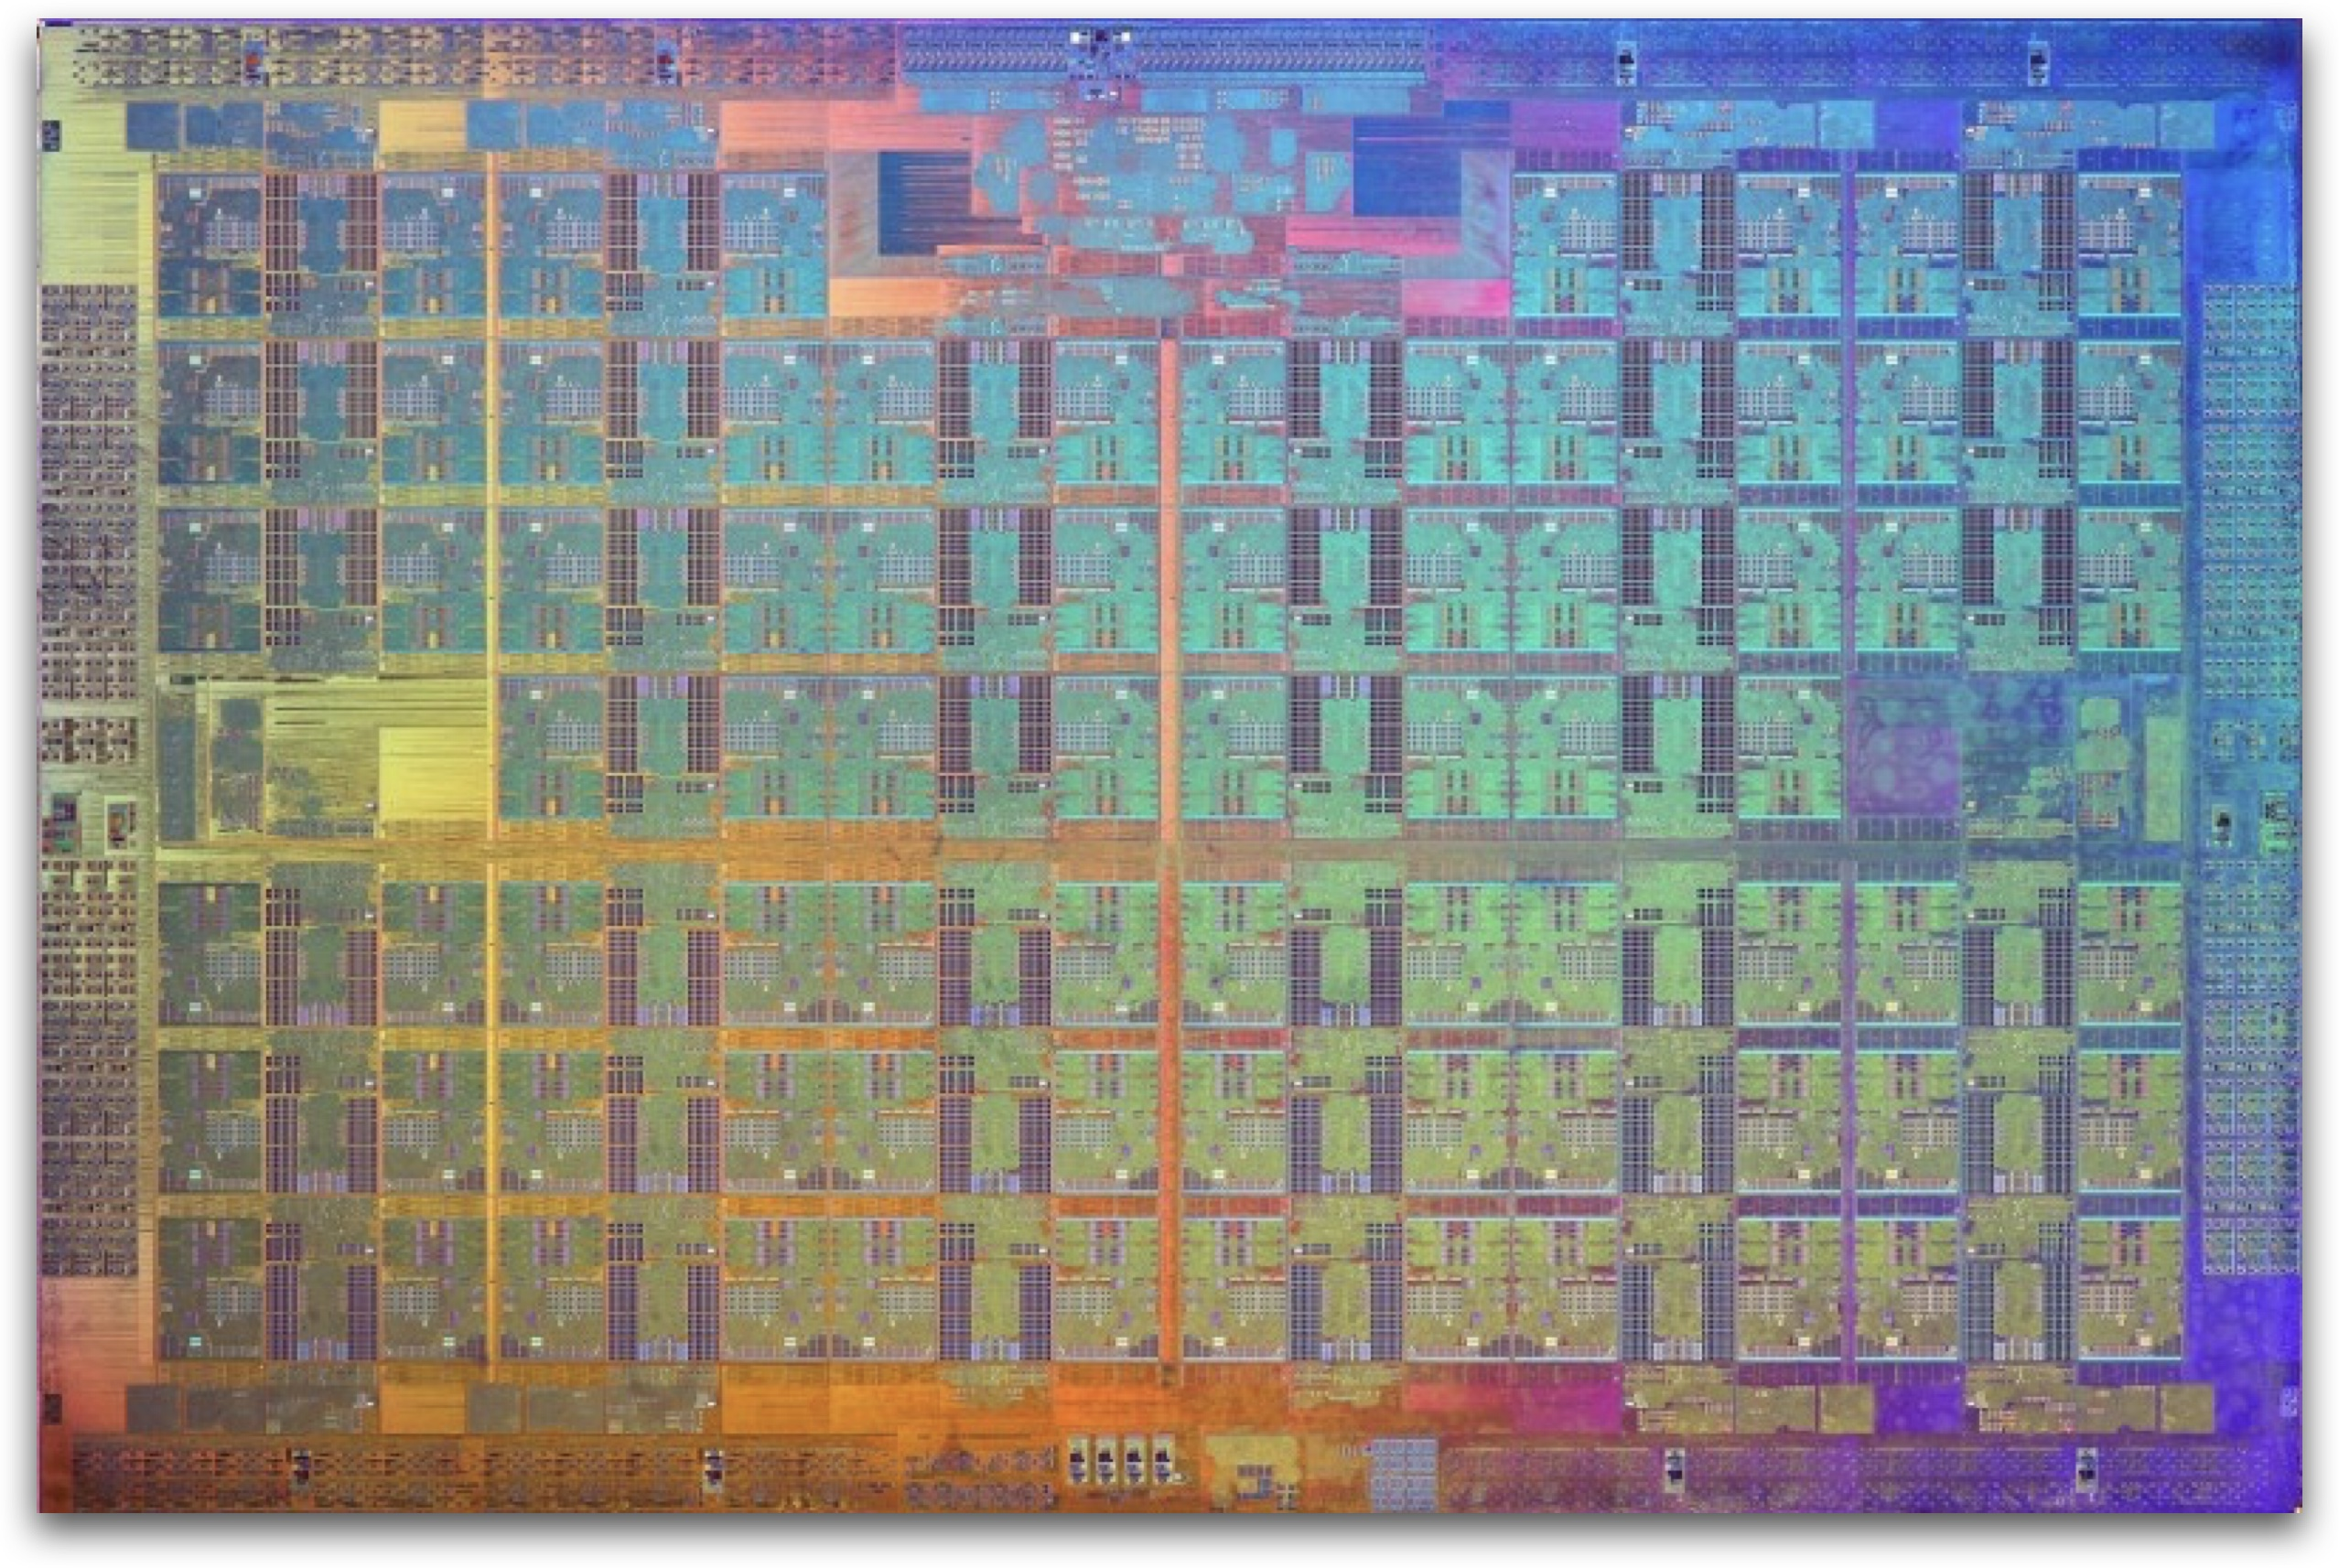
\includegraphics[height=0.75\textheight]{figures/mic_die_shot.jpg}
\end{center}
\end{frame}

\begin{frame}{Intel Xeon “Broadwell” Nodes}
\begin{itemize}
\item Dual Intel Xeon E5-2695v4 2.1 GHz 18-core ``Broadwell'' processors
\item Cache: 45 MB L3
\item Memory: DDR4 2400 MHz, 76.8 GB/s
\item Vector Extensions: AVX2 (256 bit width)
\end{itemize}
\end{frame}

\begin{frame}{Intel Xeon “Skylake” Nodes}
\begin{itemize}
\item Dual Intel Xeon Gold 6154 3.0 GHz 18-core ``Skylake'' processors
\item Cache: 24.75 MB L3
\item Memory: DDR4 2666 MHz, 119.21 GB/s
\item Vector Extensions: AVX-512 (512 bit width)
\end{itemize}
\end{frame}

\begin{frame}{NVIDIA SuperPOD DGX Nodes}
\begin{columns}
\begin{column}{0.5\textwidth}
\begin{itemize}
\item Dual AMD Epyc 7742 2.25 GHz 64-core ``Rome'' processors
\item Cache: 256 MB L3
\item Memory: DDR4 3200 MHz, 204.8 GB/s
\item Vector Extensions: AVX2 (256 bit width)
\end{itemize}
\end{column}
\begin{column}{0.5\textwidth}
\begin{center}
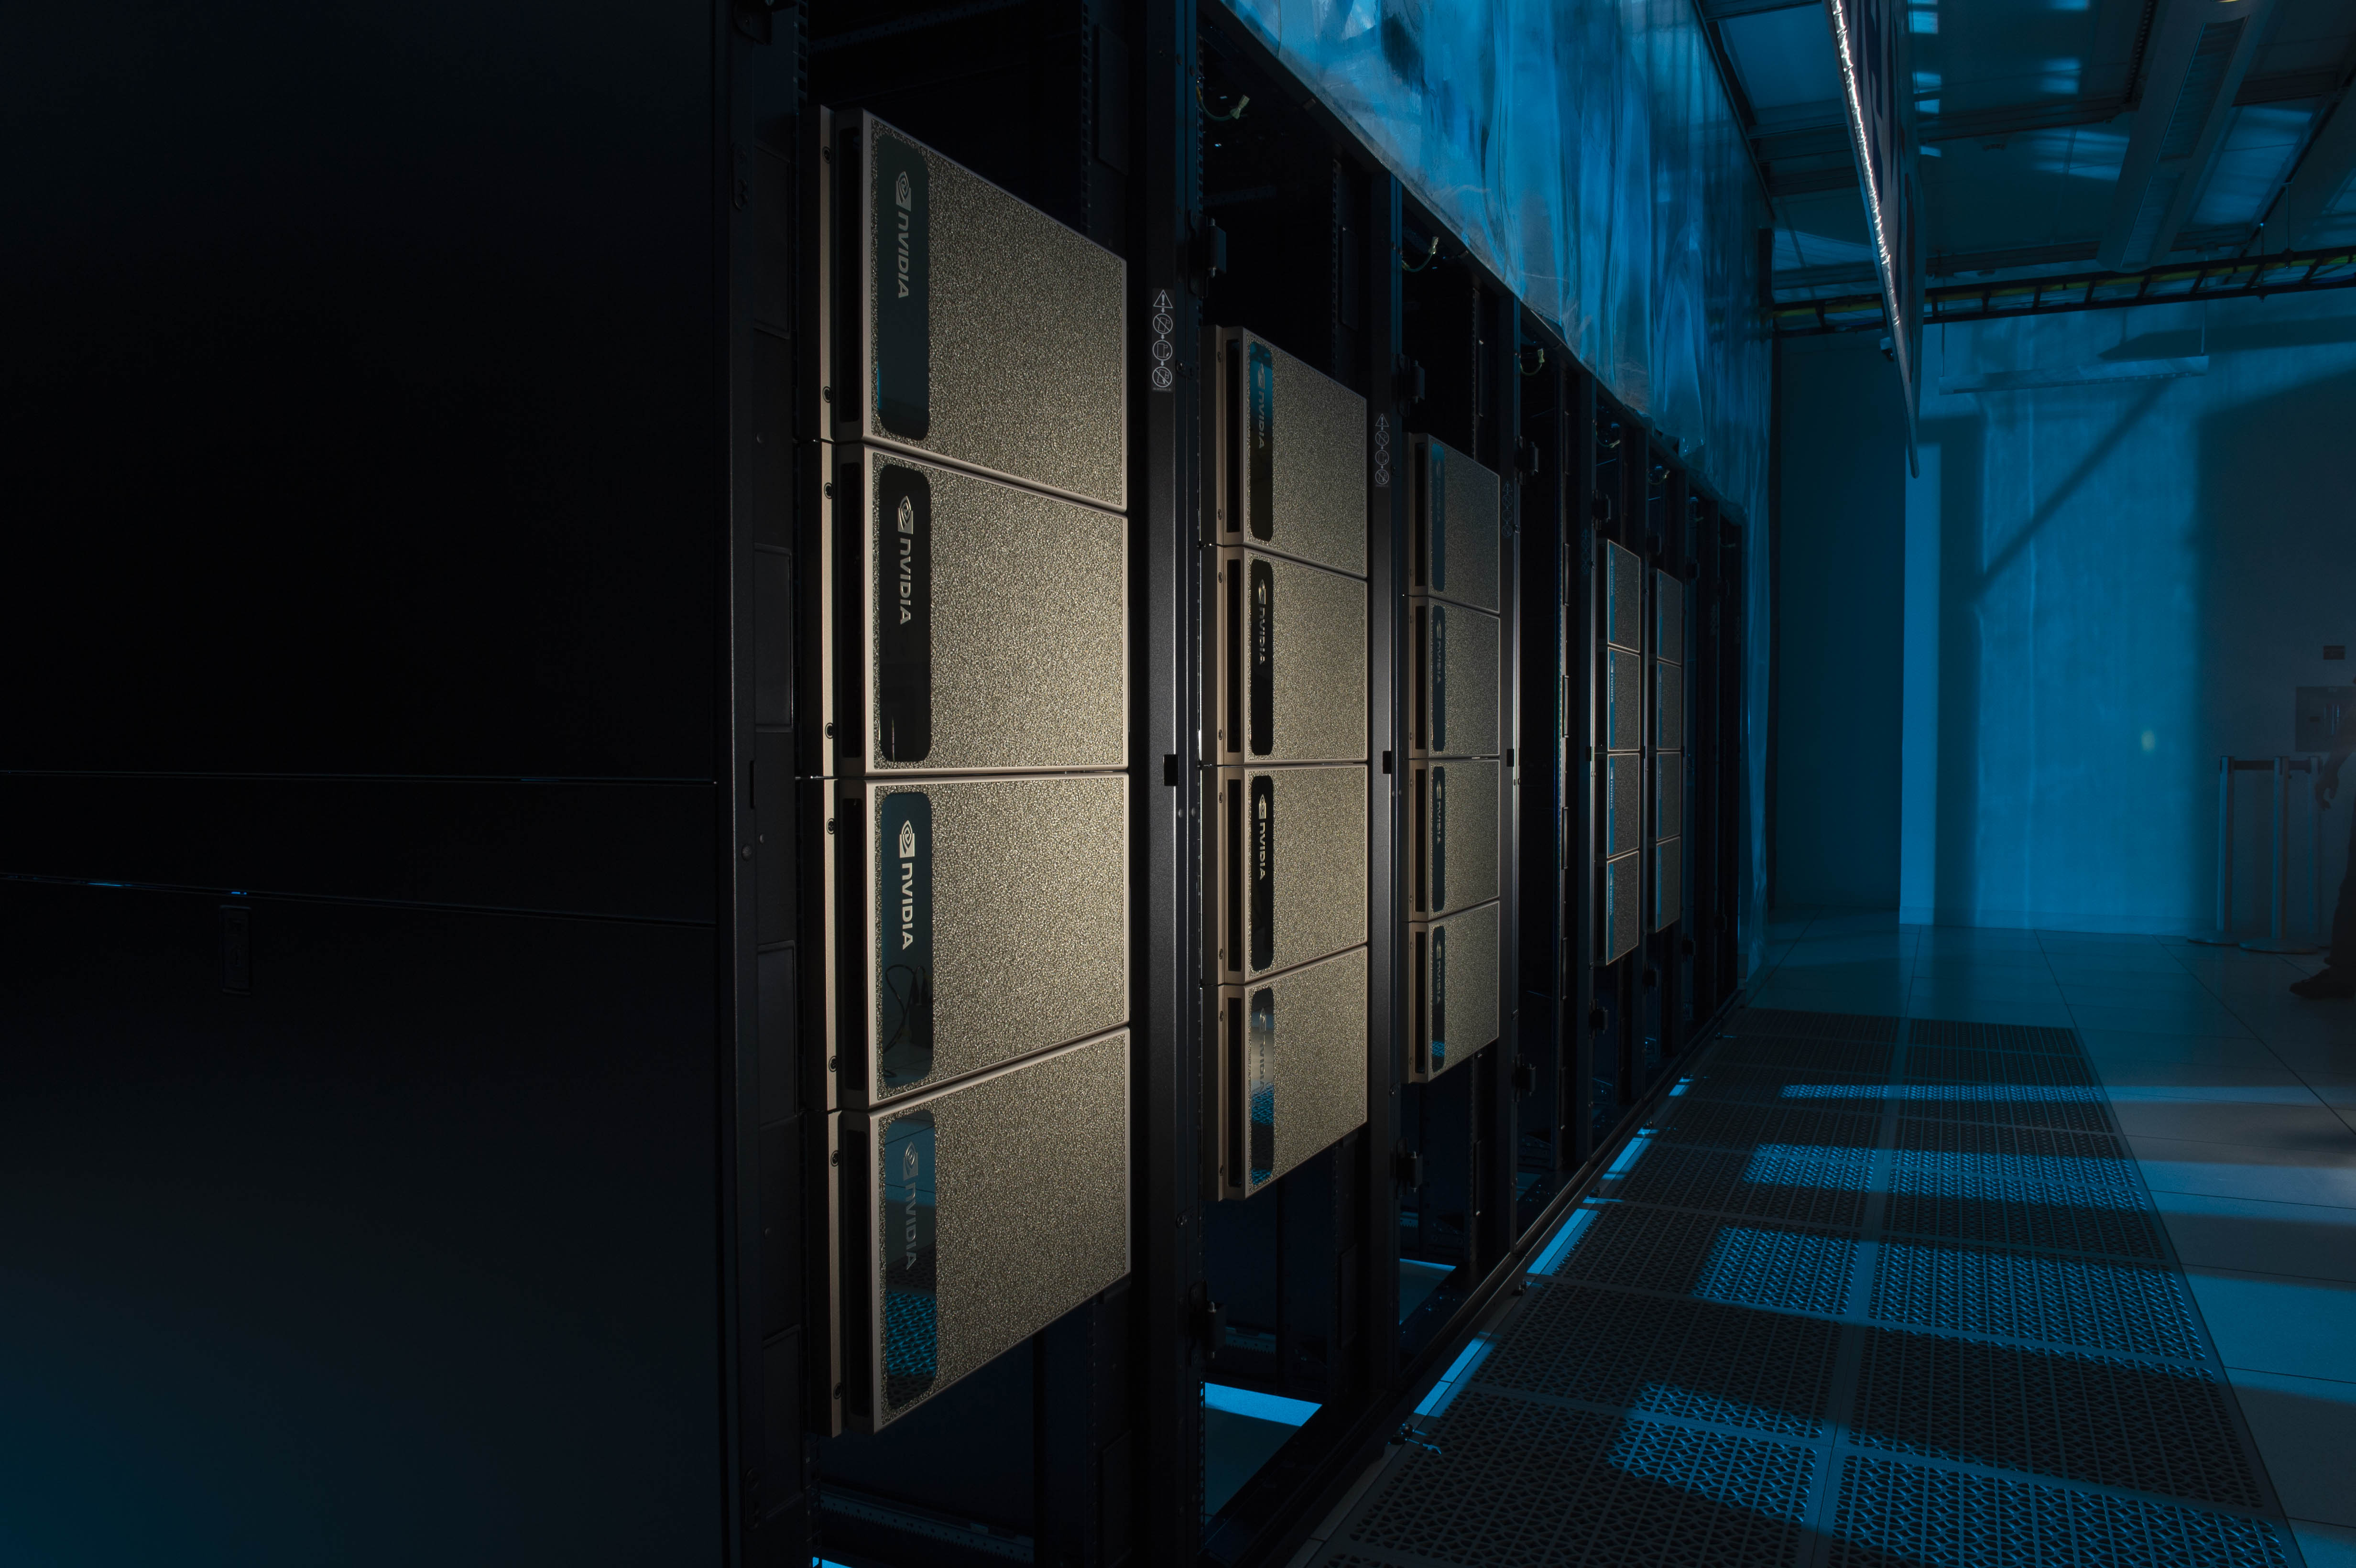
\includegraphics[width=\textwidth]{figures/superpod.jpg}
\end{center}
\end{column}
\end{columns}
\end{frame}


%\section{Vector Extensions}

\begin{frame}{Array Programming}
\begin{itemize}
   \item Operations are exclusively done over vectors, matrices, and tensors instead of scalars
   \item Scalars in array programming are vectors with a single index
   \item Array programming simplifies programming linear algebra algorithms
   \item Array programming languages include MATLAB, Octave, R, Julia, and Python via NumPy
\end{itemize}
\end{frame}

\begin{frame}[fragile]{Array Programming in Python}
\centering\small
\begin{minted}{python}
>>> from numpy import matrix, linalg
>>> A = matrix([[1,2,3],[4,5,6],[7,8,9]])
>>> x = matrix([[1],[2],[3]])
>>> print(A.T)
[[1 4 7]
 [2 5 8]
 [3 6 9]]
>>> print(A*x)
[[14]
 [32]
 [50]]
\end{minted}
\end{frame}

\begin{frame}{Single Instruction, Multiple Data}
\begin{itemize}
    \item A single operation is applied to multiple data simultaneously
    \item Allows some linear alegra operations to be done via vectors instead of single elements
    \item Modern systems are MIMD where each processor or core can perform independent SIMD operations
    \item SIMD instructions are CPU architecture specific, \textit{i.e.}\ not all CPU's have the same SIMD instruction sets
\end{itemize}
\end{frame}

\begin{frame}[fragile]{Vectorization Example}
\centering
\begin{minted}{c}
for (int i=0; i<16; ++i) {
   C[i] = A[i] + B[i];
}

for (int i=0; i<16; i+=4) {
   addFourThingsAtOnceAndStoreResult(&C[i], &A[i], &B[i]);
}
\end{minted}
\end{frame}

\begin{frame}{Advanced Vector Extensions}
\begin{itemize}
    \item Advanced Vector Extensions (AVX) are a set of SIMD extensions to the x86 instruction set
    \item Initially developed by Intel in 2008
    \item Implemented in Intel and AMD CPU's since 2011
\end{itemize}
\end{frame}

\begin{frame}{AVX Versions}
\begin{description}
   \item[AVX]
    \begin{itemize}
        \item Expanded many of the earlier SSE floating point instructions from 128 to 256 bits
        \item Several new instructions
        \item Intel Sandy Bridge and AMD Bulldozer and newer architectures
    \end{itemize}
   \item[AVX2]
    \begin{itemize}
        \item Expanded many of the earlier SSE integer instruction from 128 to 256 bits
        \item Several new instructions
        \item Intel Haswell and AMD Carrizo and newer architectures
    \end{itemize}
   \item[AVX-512]
    \begin{itemize}
        \item Expanded AVX instructions from 256 to 512 bits
        \item Several new instructions
        \item Intel Xeon Phi x200 series CPU's
    \end{itemize}
\end{description}
\end{frame}

\begin{frame}{Vector Extension Widths}
\begin{center}
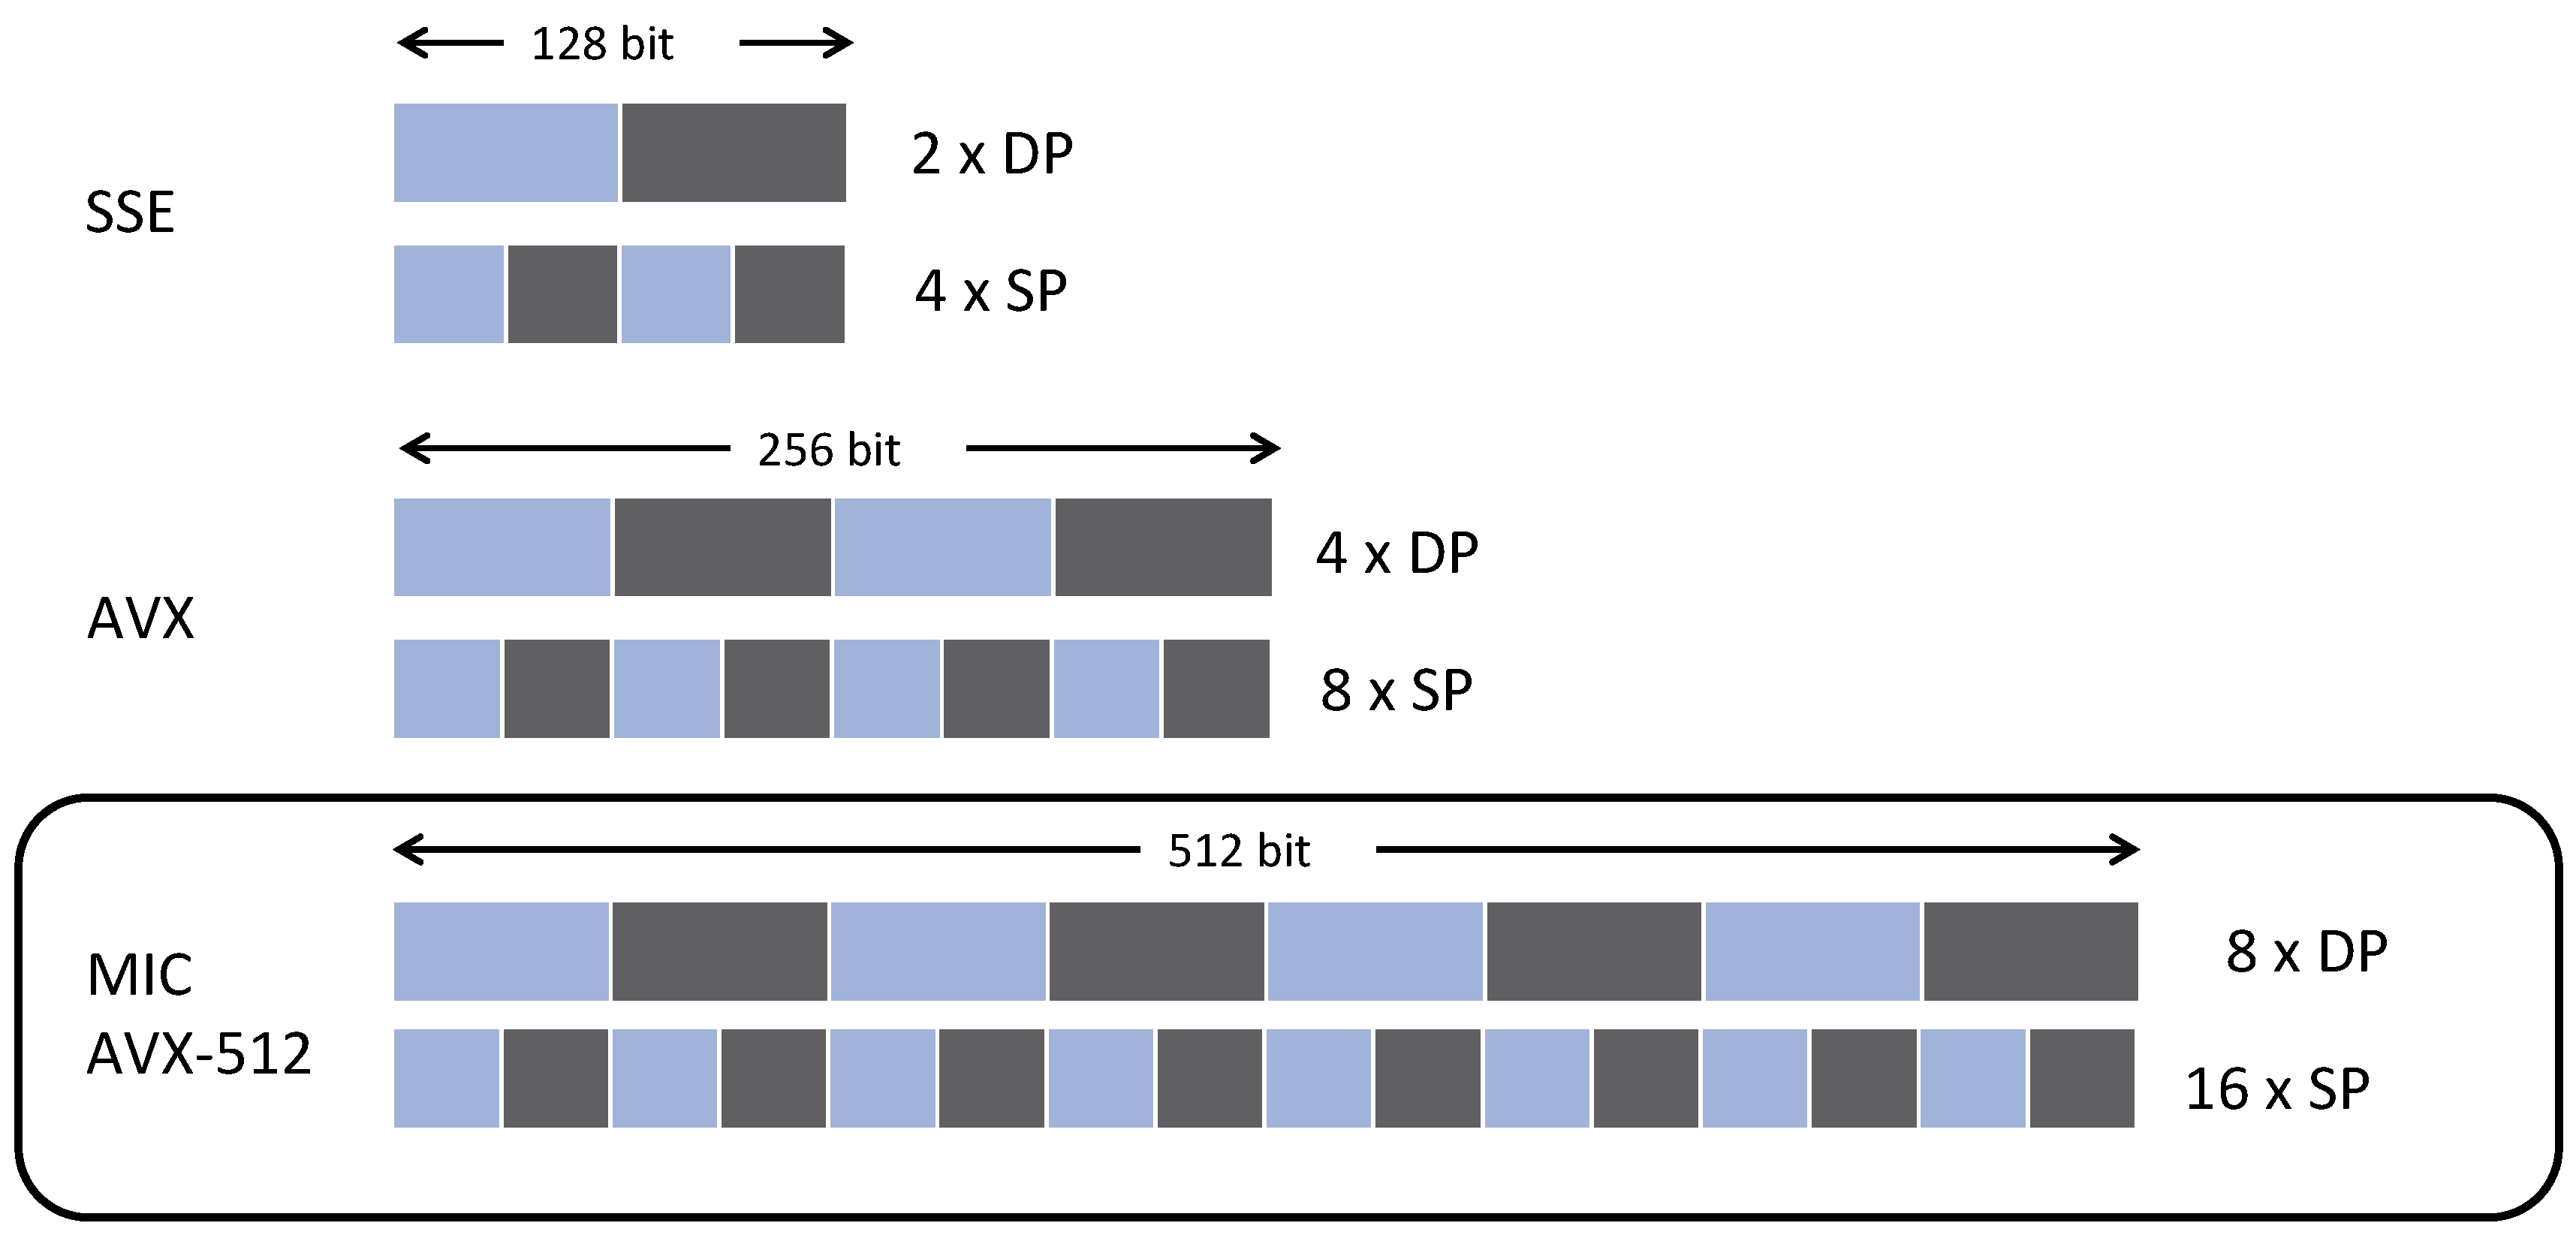
\includegraphics[width=\textwidth]{figures/vector_widths_1.pdf}
\end{center}
\end{frame}

\begin{frame}{Vector Extension Addition}
\begin{center}
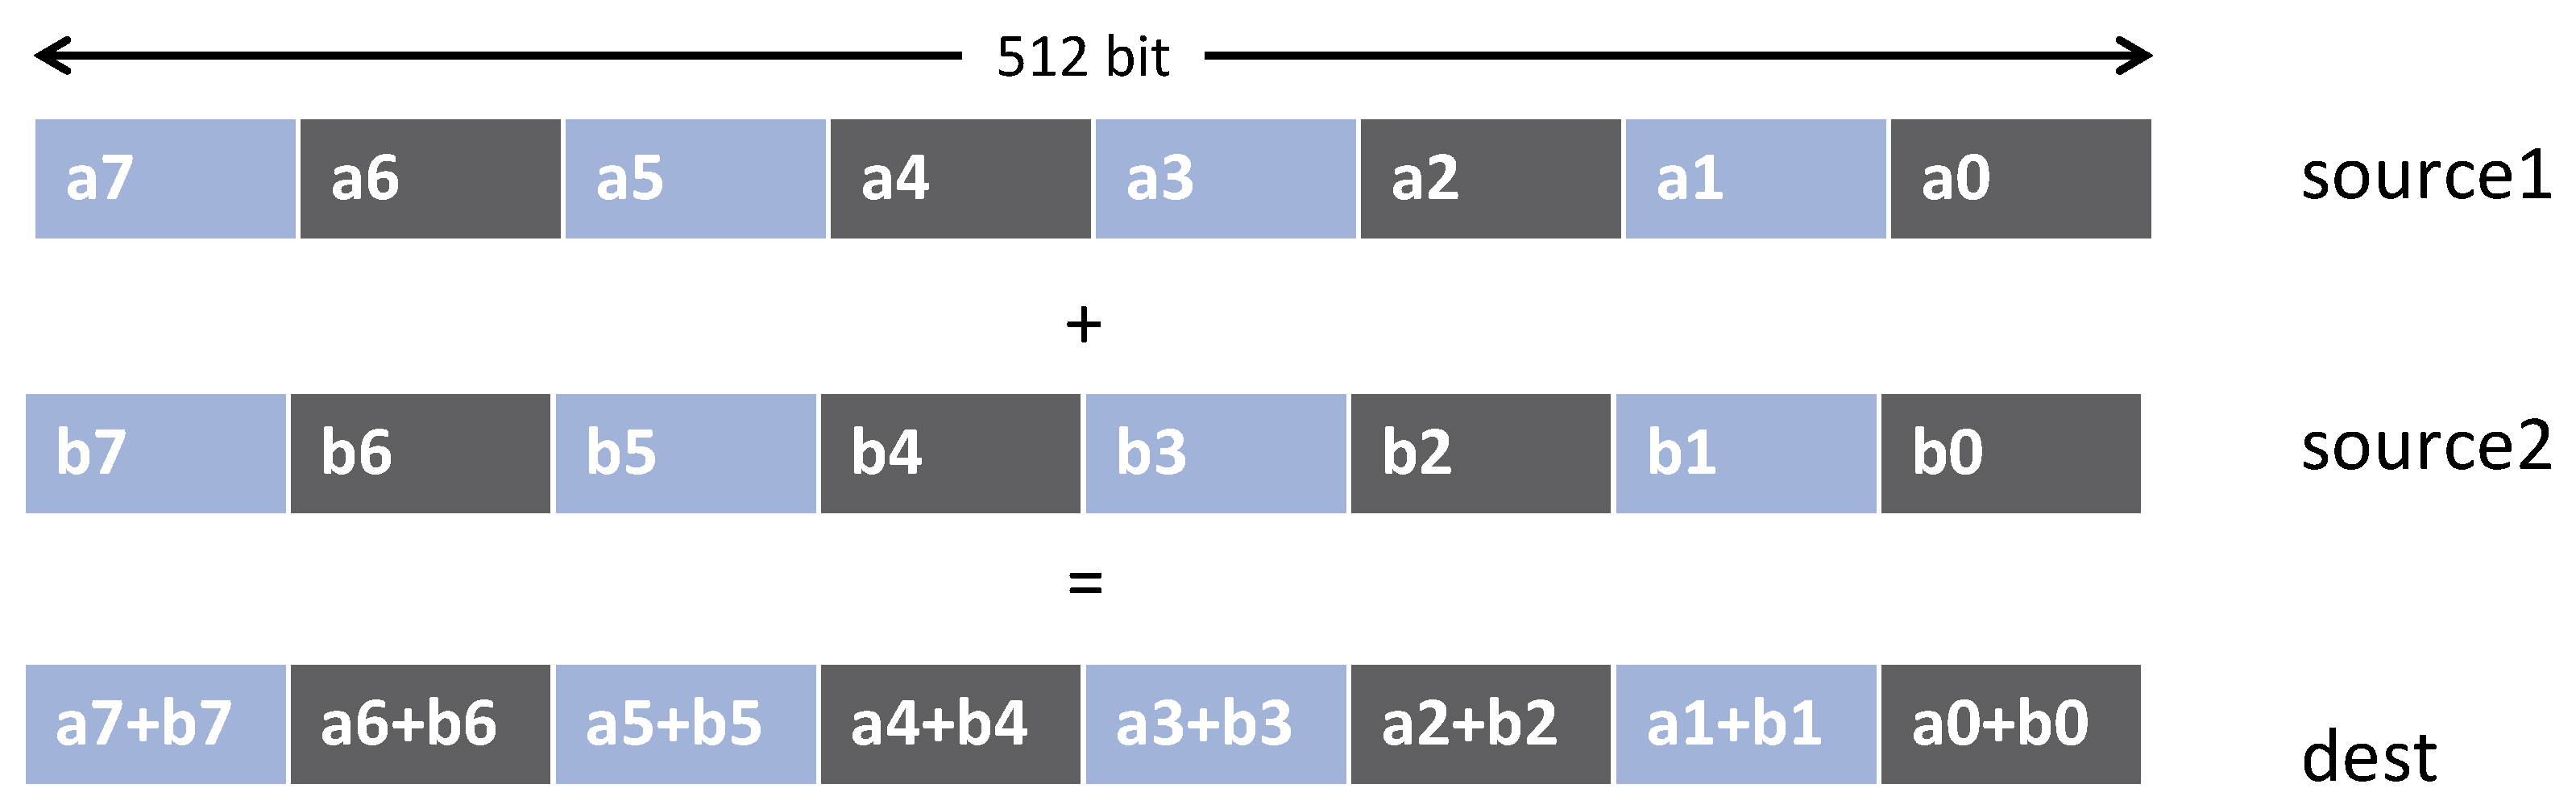
\includegraphics[width=\textwidth]{figures/vector_widths_2.pdf}
\end{center}
\end{frame}

\begin{frame}{Vector Extension Fused Multiply-Add}
\begin{center}
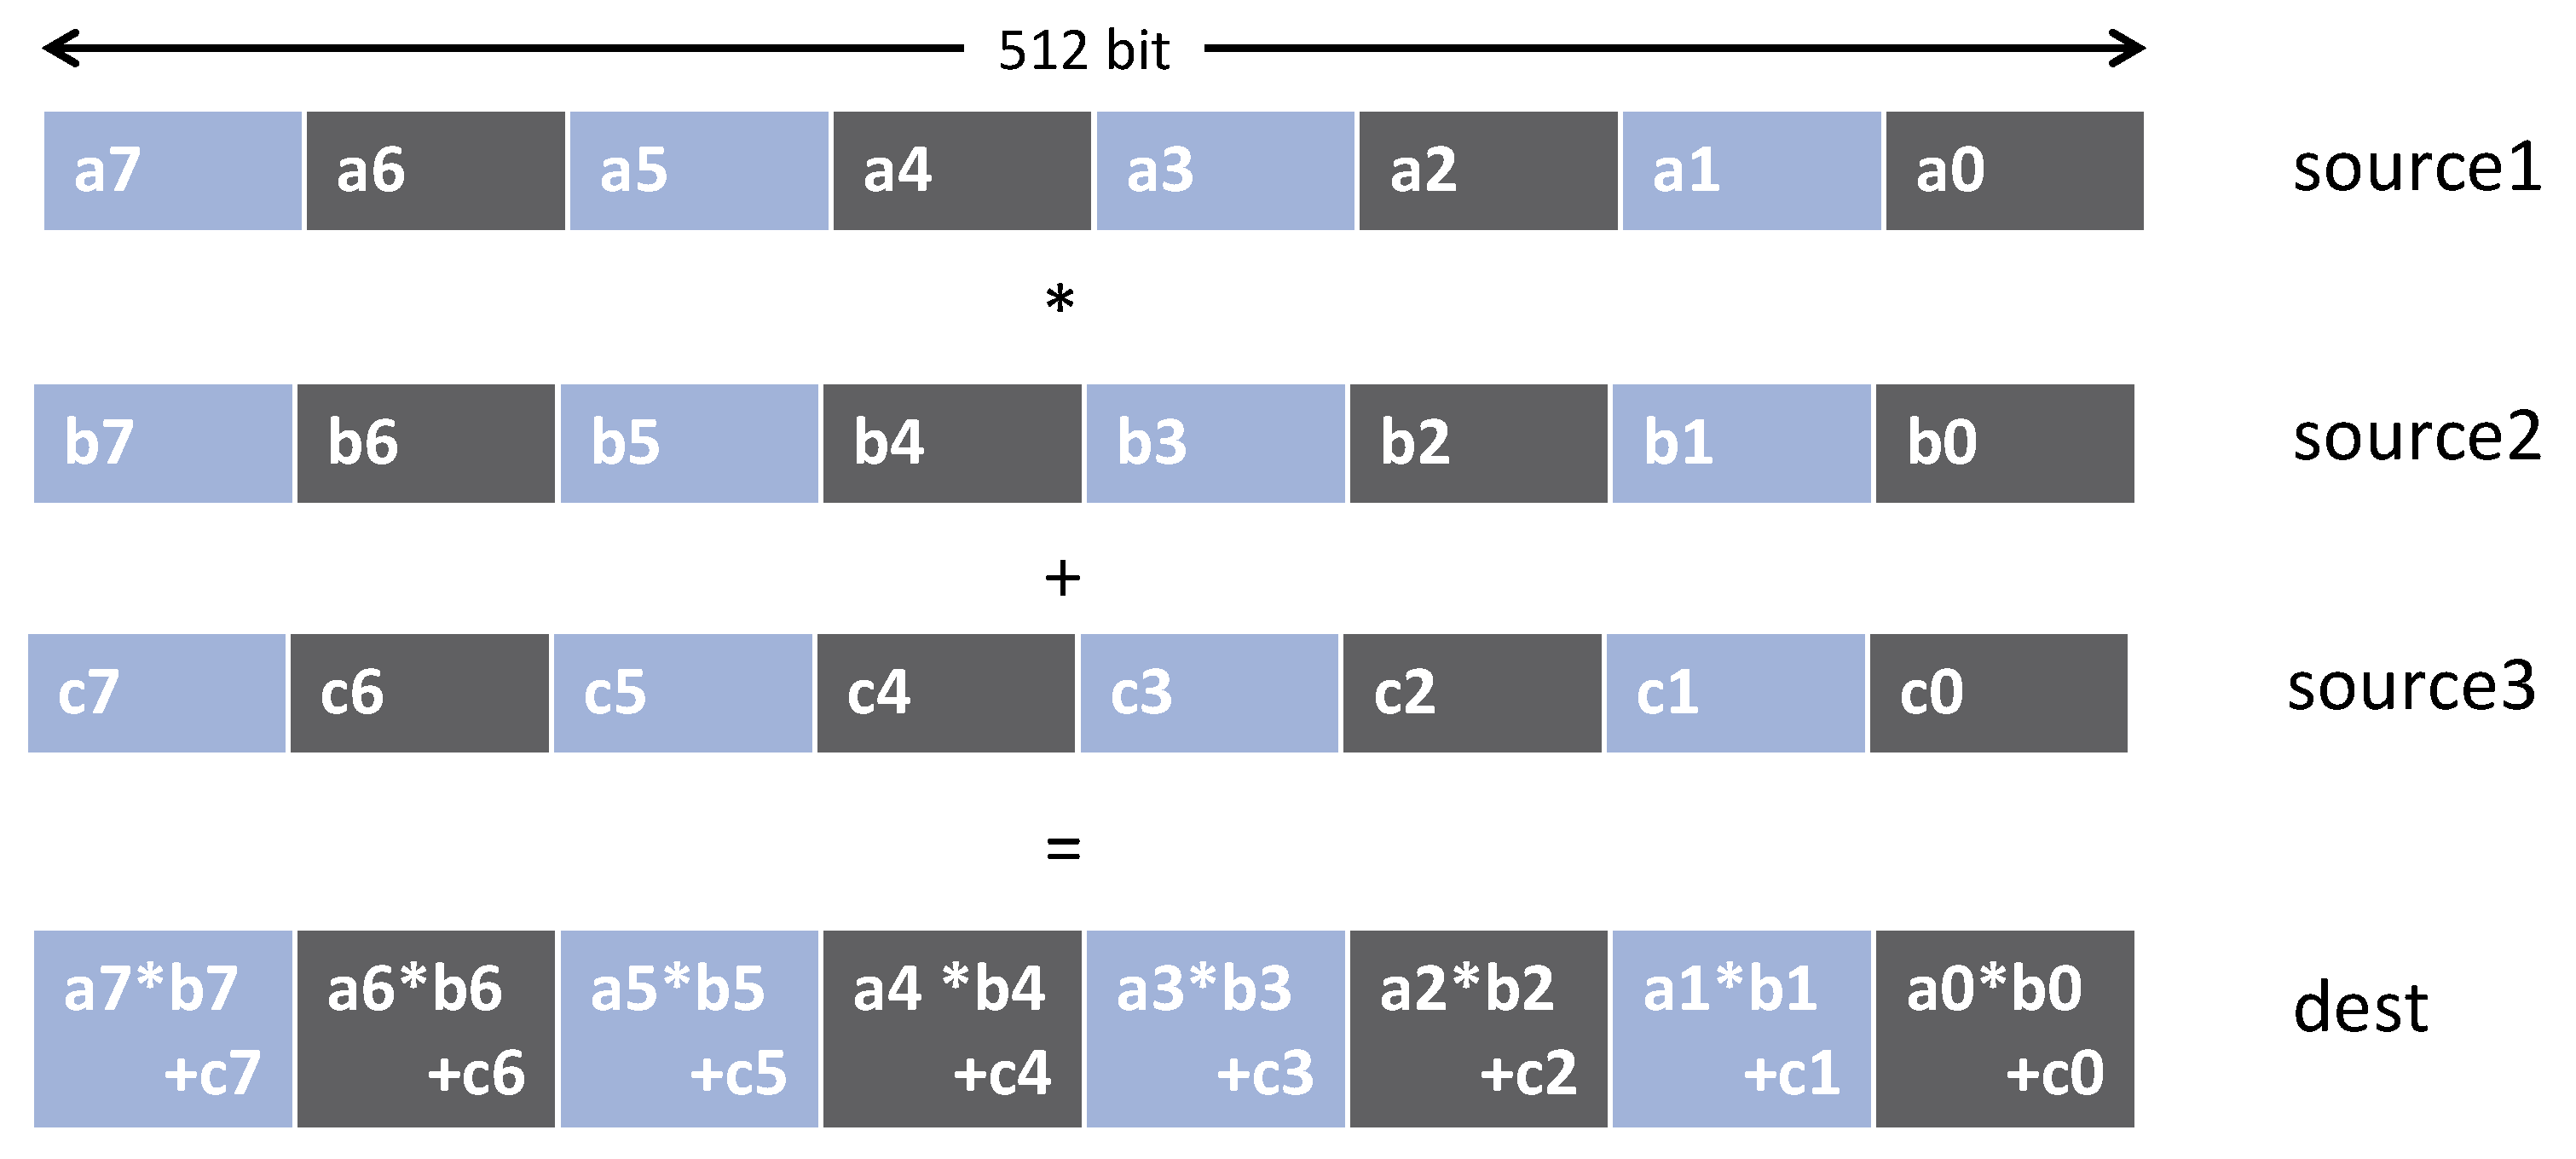
\includegraphics[width=\textwidth]{figures/vector_widths_3.pdf}
\end{center}
\end{frame}


\section{Accessing ManeFrame II (M2)}

\begin{frame}{Accessing ManeFrame II (M2)}
\begin{description}
\item[SSH]
\begin{itemize}
  \item Provides secure command line access to the login nodes.
  \item Graphical applications require X11-forwarding.
  \item Five login nodes all accessible via \mintinline{sh}{m2.smu.edu}.
  \item \href{https://s2.smu.edu/hpc/documentation/access.html}{M2 SSH Instructions}
\end{itemize}
\item[HPC Portal]
\begin{itemize}
  \item Provides web-based access to M2.
  \begin{itemize}
    \item File access
    \item Terminal access
    \item JupyterLab (Notebooks)
    \item RStudio
    \item Remote Desktops
  \end{itemize}
\end{itemize}
\item[SFTP]
\begin{itemize}
  \item Transfer files to and from M2 using an SFTP client.
  \item \href{https://s2.smu.edu/hpc/documentation/access.html}{M2 SFTP Instructions}
\end{itemize}
\end{description}
\end{frame}

\begin{frame}{ManeFrame II (M2) HPC OnDemand Web Portal}
\begin{columns}[c]
\begin{column}{0.5\textwidth}
\begin{itemize}
\item Provides an integrated single access point for HPC resources on the
ManeFrame II (M2) supercomputer
\item Accessing the Portal:
\begin{itemize}
\item Access to the HPC portal requires an existing M2 account
\item Go to \url{hpc.smu.edu}
\item Sign in using your SMU ID and SMU password
\end{itemize}
\item \href{https://s2.smu.edu/hpc/documentation/portal.html}{HPC Portal
Documentation}
\item
\href{https://s2.smu.edu/hpc/documentation/portal.html\#remote-desktop}{HPC
Portal Walkthrough Video}
\end{itemize}
\end{column}
\begin{column}{0.5\textwidth}
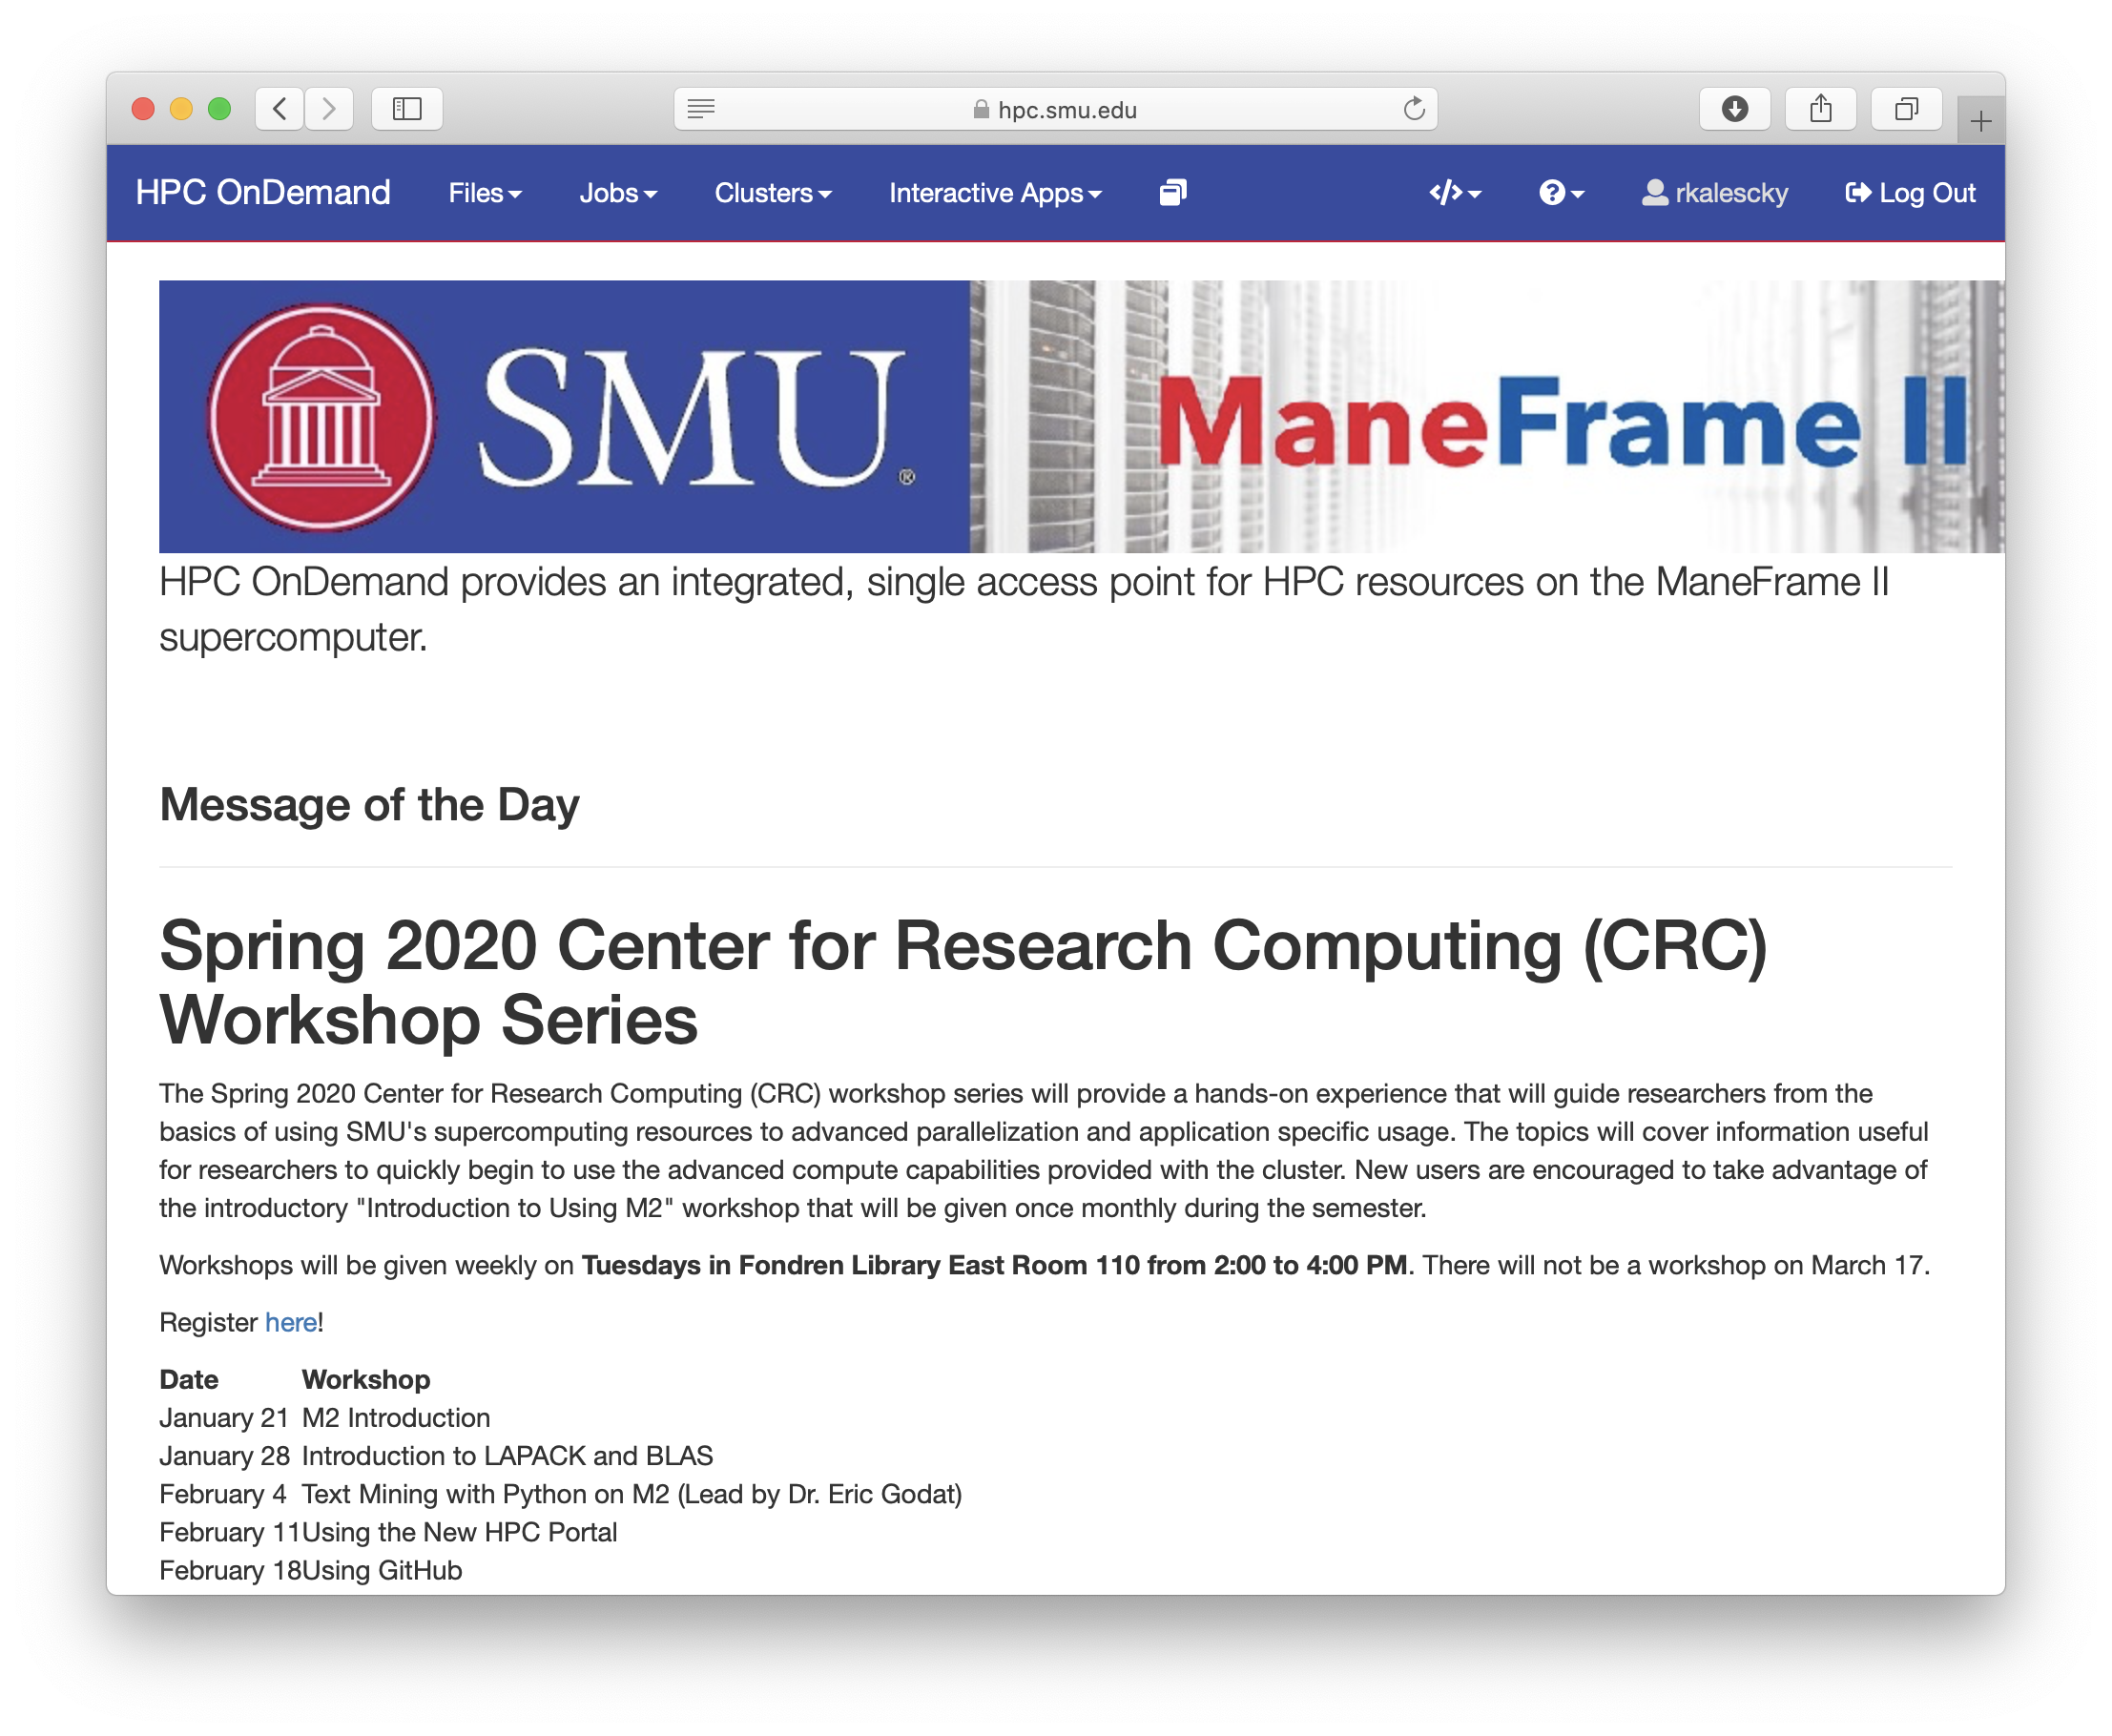
\includegraphics[width=\linewidth]{figures/portal.png}
\end{column}
\end{columns}
\end{frame}


\section{HPC Usage}

\begin{frame}{M3 Usage}
\begin{table}
\scriptsize
\begin{tabular}{lllll}
\toprule
Rank & Sponsor & Department & Job Count & Total Job Duration \\
\midrule
1 & Dr.\ Bennett & Chemistry & 2147111 & 162672 days, 10:58:28 \\
2 & Dr.\ Cooley & Physics & 148072 & 4940 days, 6:19:00 \\
3 & Dr.\ Kamata & Simmons & 25857 & 2302 days, 19:06:08 \\
4 & Dr.\ Deiana & Physics & 25689 & 472 days, 15:13:30 \\
5 & Dr.\ Matthews & Chemistry & 10826 & 884 days, 5:59:58 \\
6 & Dr.\ Meltzer & Anthropology & 7336 & 665 days, 0:44:46 \\
7 & Dr.\ Norris & Biology & 25585 & 188 days, 23:34:01 \\
8 & Dr.\ Kraka & Chemistry & 7203 & 528 days, 12:56:38 \\
9 & Dr.\ Stroynowski & Physics & 35893 & 77 days, 12:02:47 \\
10 & Dr.\ Borbolla & Mathematics & 1807 & 719 days, 15:43:02 \\
\bottomrule
\end{tabular}
\end{table}
\end{frame}

\begin{frame}{MP Usage}
\begin{table}
\scriptsize
\begin{tabular}{lllll}
\toprule
Rank & Sponsor & Department & Job Count & Total Job Duration \\
\midrule
1 & Dr.\ Zoltowski & Chemistry & 1960 & 1204 days, 13:33:12 \\
2 & Dr.\ Tao & Chemistry  & 2354 & 785 days, 22:05:11 \\
3 & Dr.\ Kraka & Chemistry & 1504 & 840 days, 12:45:19 \\
4 & Dr.\ Roy & Economics & 10874 & 62 days, 05:52:17 \\
5 & Dr.\ Guldi & History & 934 & 320 days, 08:10:47 \\
6 & Dr.\ Deiana & Physics & 6344 & 31 days, 03:51:10 \\
7 & Dr.\ Larson & Computer Science & 1429 & 83 days, 06:40:00 \\
8 & Dr.\ Godat & OIT & 1616 & 66 days, 19:59:13 \\
9 & Dr.\ Meyers & Physics & 843 & 95 days, 22:25:10 \\
10 & Dr.\ Brenner & Electrical Engineering & 276 & 84 days, 11:50:43 \\
\bottomrule
\end{tabular}
\end{table}
\end{frame}



\section{Resource Management Via Slurm}

\begin{frame}{Cluster Resource Management}
\begin{itemize}
\item Compute resources are shared by all users
\item Queue systems manage access to specific resources
\item There are many queue systems around: Moab, Torque, LoadLeveler, Condor,
      Oracle Grid Engine, Argent Job Scheduler, Platform LSF, etc.
\item SMU HPC clusters uses Simple Linux Utility for Resource Management
      (SLURM)
\end{itemize}
\end{frame}

\begin{frame}{Cluster Resource Management}
\begin{itemize}
\item SMU HPC resource allocation is governed by a fair-share factor
\begin{itemize}
\item Preference is given to those who have submitted the fewest jobs
\item Prevents a single user from “blocking” subsequent job submissions of
      other users
\end{itemize}
\item Allocations can be requested interactively or as a batch job
\item Queues (or partitions) are used to distinguish resources by type and the
      maximum run time
\end{itemize}
\end{frame}

\begin{frame}{M3 Partitions (Queues)}
\begin{table}
\scriptsize
\begin{tabular}{llll}
\toprule
Partition & Duration & Cores & Memory [GB]\\
\midrule
dev & 2 hours & various & various\\
htc & 1 day & 1 & 3.9\\
standard-s & 1 day & 128 & 512\\
standard-l & 1 week & 128 & 512\\
highmem & 5 days & 128 & 2048\\
\bottomrule
\end{tabular}
\end{table}
\end{frame}

\begin{frame}{MP Partitions (Queues)}
\begin{table}
\scriptsize
\begin{tabular}{lllll}
\toprule
Partition & Duration & Cores & GPUs & Memory [GB]\\
\midrule
default & 2 days & 16 & 1 & 96\\
\bottomrule
\end{tabular}
\end{table}
\end{frame}

%\begin{frame}{Basic SLURM Commands}
%\begin{table}
%\tiny
%\begin{tabular}{lll}
%\toprule
%Command & Description & Example Usage\\
%\midrule
%sinfo & Displays partition and node state information & \mintinline{sh}{sinfo}\\
%squeue & Displays queue state information & \mintinline{sh}{squeue -u $USER}\\
%sbatch & Submits batch script & \mintinline{sh}{sbatch job.submit}\\
%srun & Requests resources for interactive use & \mintinline{sh}{srun -p dev -c 1 --mem=1G --pty $SHELL}\\
%scancel & Cancel jobs & \mintinline{sh}{scancel 12345678}\\
%\bottomrule
%\end{tabular}
%\end{table}
%\end{frame}

\section{Demo}

\section{Tour}



%\section{Slurm}

\begin{frame}{Serial Python Script: \(\pi\) Monte Carlo}
\begin{listing}[H]
\inputminted{python}{examples/slurm_tutorial/pi_monte_carlo.py}
\caption{Serial algorithm to estimate the value of \(\pi\).}
\end{listing}
\end{frame}

\begin{frame}{Parallel Python Script: \(\pi\) Monte Carlo}
\begin{listing}[H]
\inputminted[fontsize=\tiny]{python}{examples/slurm_tutorial/pi_monte_carlo_shared.py}
\caption{Parallel algorithm to estimate the value of \(\pi\).}
\end{listing}
\end{frame}

\begin{frame}{Interactive Sessions}
\begin{listing}[H]
\inputminted{sh}{examples/slurm_tutorial/01_interactive_session}
\caption{Using \mintinline{sh}{srun} to log into a compute node to run commands interactively.}
\end{listing}
\end{frame}

\begin{frame}{Using \mintinline{sh}{srun}}
\begin{listing}[H]
\inputminted{sh}{examples/slurm_tutorial/02_srun}
\caption{Using \mintinline{sh}{srun} to run commands directly on a compute node.}
\end{listing}
\end{frame}

\begin{frame}{Using \mintinline{sh}{sbatch --wrap}}
\begin{listing}[H]
\inputminted{sh}{examples/slurm_tutorial/03_sbatch_wrap}
\caption{Using \mintinline{sh}{sbatch --wrap} wrap a commands in an \mintinline{sh}{sbatch} script that is then submitted to the queue can run non-interactively.}
\end{listing}
\end{frame}

\begin{frame}{Using \mintinline{sh}{sbatch}}
\begin{listing}[H]
\inputminted{sh}{examples/slurm_tutorial/04_sbatch_htc.sbatch}
\caption{Using \mintinline{sh}{sbatch} run serial computations via an \mintinline{sh}{sbatch} script.}
\end{listing}
\end{frame}

\begin{frame}{Using \mintinline{sh}{sbatch}}
\begin{listing}[H]
\inputminted{sh}{examples/slurm_tutorial/05_sbatch_standard-mem-s.sbatch}
\caption{Using \mintinline{sh}{sbatch} run parallel computations via an \mintinline{sh}{sbatch} script.}
\end{listing}
\end{frame}

\begin{frame}{Using \mintinline{sh}{sbatch --array}}
\begin{listing}[H]
\inputminted{sh}{examples/slurm_tutorial/06_sbatch_array.sbatch}
\caption{Using \mintinline{sh}{sbatch --array} run parallel jobs via a single \mintinline{sh}{sbatch} script.}
\end{listing}
\end{frame}


%\section{Slurm}

\begin{frame}{Serial R Script: \(\pi\) Monte Carlo}
\begin{listing}[H]
\inputminted{R}{examples/r_workflows/pi_monte_carlo_serial.R}
\caption{Serial algorithm to estimate the value of Pi.}
\end{listing}
\end{frame}

\begin{frame}{Parallel R Script: \(\pi\) Monte Carlo}
\begin{listing}[H]
\inputminted{R}{examples/r_workflows/pi_monte_carlo_parallel.R}
\caption{Parallel algorithm to estimate the value of Pi.}
\end{listing}
\end{frame}

\begin{frame}{Interactive Sessions}
\begin{listing}[H]
\inputminted{sh}{examples/r_workflows/01_interactive_session}
\caption{Using \mintinline{sh}{srun} to log into a compute node to run commands interactively.}
\end{listing}
\end{frame}

\begin{frame}{Using \mintinline{sh}{srun}}
\begin{listing}[H]
\inputminted{sh}{examples/r_workflows/02_srun}
\caption{Using \mintinline{sh}{srun} to run commands directly on a compute node.}
\end{listing}
\end{frame}

\begin{frame}{Using \mintinline{sh}{sbatch --wrap}}
\begin{listing}[H]
\inputminted{sh}{examples/r_workflows/03_sbatch_wrap}
\caption{Using \mintinline{sh}{sbatch --wrap} wrap a commands in an \mintinline{sh}{sbatch} script that is then submitted to the queue can run non-interactively.}
\end{listing}
\end{frame}

\begin{frame}{Using \mintinline{sh}{sbatch}}
\begin{listing}[H]
\inputminted{sh}{examples/r_workflows/04_sbatch_htc.sbatch}
\caption{Using \mintinline{sh}{sbatch} run serial computations via an \mintinline{sh}{sbatch} script.}
\end{listing}
\end{frame}

\begin{frame}{Using \mintinline{sh}{sbatch}}
\begin{listing}[H]
\inputminted{sh}{examples/r_workflows/05_sbatch_standard-mem-s.sbatch}
\caption{Using \mintinline{sh}{sbatch} run parallel computations via an \mintinline{sh}{sbatch} script.}
\end{listing}
\end{frame}

\begin{frame}{Using \mintinline{sh}{sbatch --array}}
\begin{listing}[H]
\inputminted{sh}{examples/r_workflows/06_sbatch_array.sbatch}
\caption{Using \mintinline{sh}{sbatch --array} run parallel jobs via a single \mintinline{sh}{sbatch} script.}
\end{listing}
\end{frame}


%\section{Python Environments}

\begin{frame}{Managing Python Installations}
\begin{itemize}
\item Python environments allow users to use specific versions of Python with
the packages of their choice
\item The packages can be installed via \mintinline{sh}{conda} or
\mintinline{sh}{pip}, depending on the type of environment being used
\end{itemize}
\end{frame}

\begin{frame}{Anaconda Environments}
\begin{itemize}
\item Anaconda environments are managed using \mintinline{sh}{conda}, which is
available via Anaconda installations such as \mintinline{sh}{python/2} and
\mintinline{sh}{python/3} on ManeFrame II.
\end{itemize}
\end{frame}

\begin{frame}{Anaconda Environments Example}
\begin{listing}[H]
\inputminted[firstline=3,firstnumber=1]{sh}{examples/conda_environments.sh}
\caption{A specific version of Python is installed along with the JupyterLab
package and its dependencies. The new environment is then loaded and then
unloaded.}
\end{listing}
\end{frame}

\begin{frame}{Python Virtual Environments}
\begin{itemize}
\item Python 3 has native support for managing environments, which can be used
with any Python 3 installation on ManeFrame II.
\end{itemize}
\end{frame}

\begin{frame}{Python Virtual Environments Example}
\begin{listing}[H]
\inputminted[firstline=3,firstnumber=1]{sh}{examples/python_environments.sh}
\caption{A specific installation of Python, in this case from Spack, is used
and then JupyterLab and its dependencies are installed. The new environment is
then loaded and then unloaded.}
\end{listing}
\end{frame}


%\section{R Environments}

\begin{frame}{\mintinline{sh}{renv} Basics}
\begin{description}
\item[\mintinline{R}{renv::init()}] Initialize new project-local environment with a private R library
\item[\mintinline{R}{renv::snapshot()}] Save the current state of the project library
\item[\mintinline{R}{renv::restore()}] Restore the previously saved state of the project library, e.g.\ reloading the environment on another machine
\end{description}
\end{frame}

\begin{frame}{GitHub and \mintinline{sh}{renv} Demo}
\begin{enumerate}
\item Create new Git repository on GitHub
\item Clone the new repository on M2
\item Create new RStudio project in RStudio via M2's Portal
\item Create clean package environment via \mintinline{R}{renv::init(bare = TRUE)}
\item Install custom packages, e.g. \mintinline{R}{renv::install("mcmc")}
\item Create environment snapshot via \mintinline{R}{renv::snapshot(packages="mcmc")}
\item Commit and push changes to the Git repository
\end{enumerate}
\end{frame}


%\section{Development Best Practices}

\begin{frame}{Best Practices}
\begin{itemize}
\item Use Git for version control
\item Use language-specific environments for package versioning
\end{itemize}
\end{frame}

\begin{frame}{GitHub}
\begin{itemize}
\item GitHub (\url{https://github.com}) is a great tool for working with Git repositories
\item Use or add your SMU email address to your GitHub account to access all GitHub Enterprise features
\end{itemize}
\end{frame}


%\section{NVSHMEM}

\begin{frame}{Motivation for NVSHMEM}
\begin{itemize}
\item Programming model for efficient and scalable multi-GPU codes.
\item Based on OpenSHMEM.
\item Provides a partitioned global address space (PGAS) that spans the memory
      of all included GPUs.
\item Communication is initiated directly from the GPUs, which can be more
      performant than CPU-bound distributed programming models.
\end{itemize}
\end{frame}

\subsection{Examples}
\subsubsection{Estimating \(\pi\)}

\begin{frame}{Estimating \(\pi\)}
\begin{listing}[H]
\inputminted[firstline=1, lastline=14]{C++}{examples/nvshmem/nvshmem_pi.cpp}
\caption{Includes and definitions.}
\end{listing}
\end{frame}

\begin{frame}{Estimating \(\pi\)}
\begin{listing}[H]
\inputminted[firstline=16, lastline=32]{C++}{examples/nvshmem/nvshmem_pi.cpp}
\caption{Monte Carlo method for estimating \(\pi\) CUDA kernel.}
\end{listing}
\end{frame}

\begin{frame}{Estimating \(\pi\)}
\begin{listing}[H]
\inputminted[firstline=35, lastline=45]{C++}{examples/nvshmem/nvshmem_pi.cpp}
\caption{Initialize NVSHMEM and get local processing element (PE) ID and global number of PEs.}
\end{listing}
\end{frame}

\begin{frame}{Estimating \(\pi\)}
\begin{listing}[H]
\inputminted[firstline=47, lastline=53]{C++}{examples/nvshmem/nvshmem_pi.cpp}
\caption{Allocate memory on hosts and devices and initialize the number of hits.}
\end{listing}
\end{frame}

\begin{frame}{Estimating \(\pi\)}
\begin{listing}[H]
\inputminted[firstline=55, lastline=65]{C++}{examples/nvshmem/nvshmem_pi.cpp}
\caption{Launch kernel on the devices to perform the computations, block until
all are finished, and then accumulate the results.}
\end{listing}
\end{frame}

\begin{frame}{Estimating \(\pi\)}
\begin{listing}[H]
\inputminted[firstline=67, lastline=77]{C++}{examples/nvshmem/nvshmem_pi.cpp}
\caption{Only on the first PE, copy accumlated hits back to host and report estimated value of \(\pi\).}
\end{listing}
\end{frame}

\begin{frame}{Estimating \(\pi\)}
\begin{listing}[H]
\inputminted[firstline=79, lastline=87]{C++}{examples/nvshmem/nvshmem_pi.cpp}
\caption{Free memory on hosts and device, finalize NVSHMEM, and exit.}
\end{listing}
\end{frame}

\begin{frame}{Estimating \(\pi\)}
\begin{listing}[H]
\inputminted[firstline=1, lastline=8]{Bash}{examples/nvshmem/nvshmem_pi.sbatch}
\caption{Reguest compute resources.}
\end{listing}
\end{frame}

\begin{frame}{Estimating \(\pi\)}
\begin{listing}[H]
\inputminted[firstline=10, lastline=16]{sh}{examples/nvshmem/nvshmem_pi.sbatch}
\caption{Setup the environment. \mintinline{sh}{$GCC_HOME} is to provide full C++ 11 support.}
\end{listing}
\end{frame}

\begin{frame}{Estimating \(\pi\)}
\begin{listing}[H]
\inputminted[firstline=18, lastline=25]{sh}{examples/nvshmem/nvshmem_pi.sbatch}
\caption{Build the executable for the specific PE being used and run.}
\end{listing}
\end{frame}


\begin{frame}{Help?}
\centering
Need help or have questions?\\
\href{mailto:rkalescky@smu.edu}{rkalescky@smu.edu} \\
\href{mailto:jlagrone@smu.edu}{jlagrone@smu.edu} \\
\href{mailto:help@smu.edu}{help@smu.edu}  (include HPC in the subject line)
\end{frame}



\end{document}

